\section{Non signal testing of the regular and variational Autoencoder}

\subsection*{Channel removing}

Both the large and small regular and variational autoencoder produced results, and are shown below. The Higgs, singletop and ttbar channels have been selected here, as they are 
from a physics stand point the channels that looks most unlike the other channels.  


\begin{figure}[h!]
    \centering
    \begin{subfigure}{.45\textwidth}
        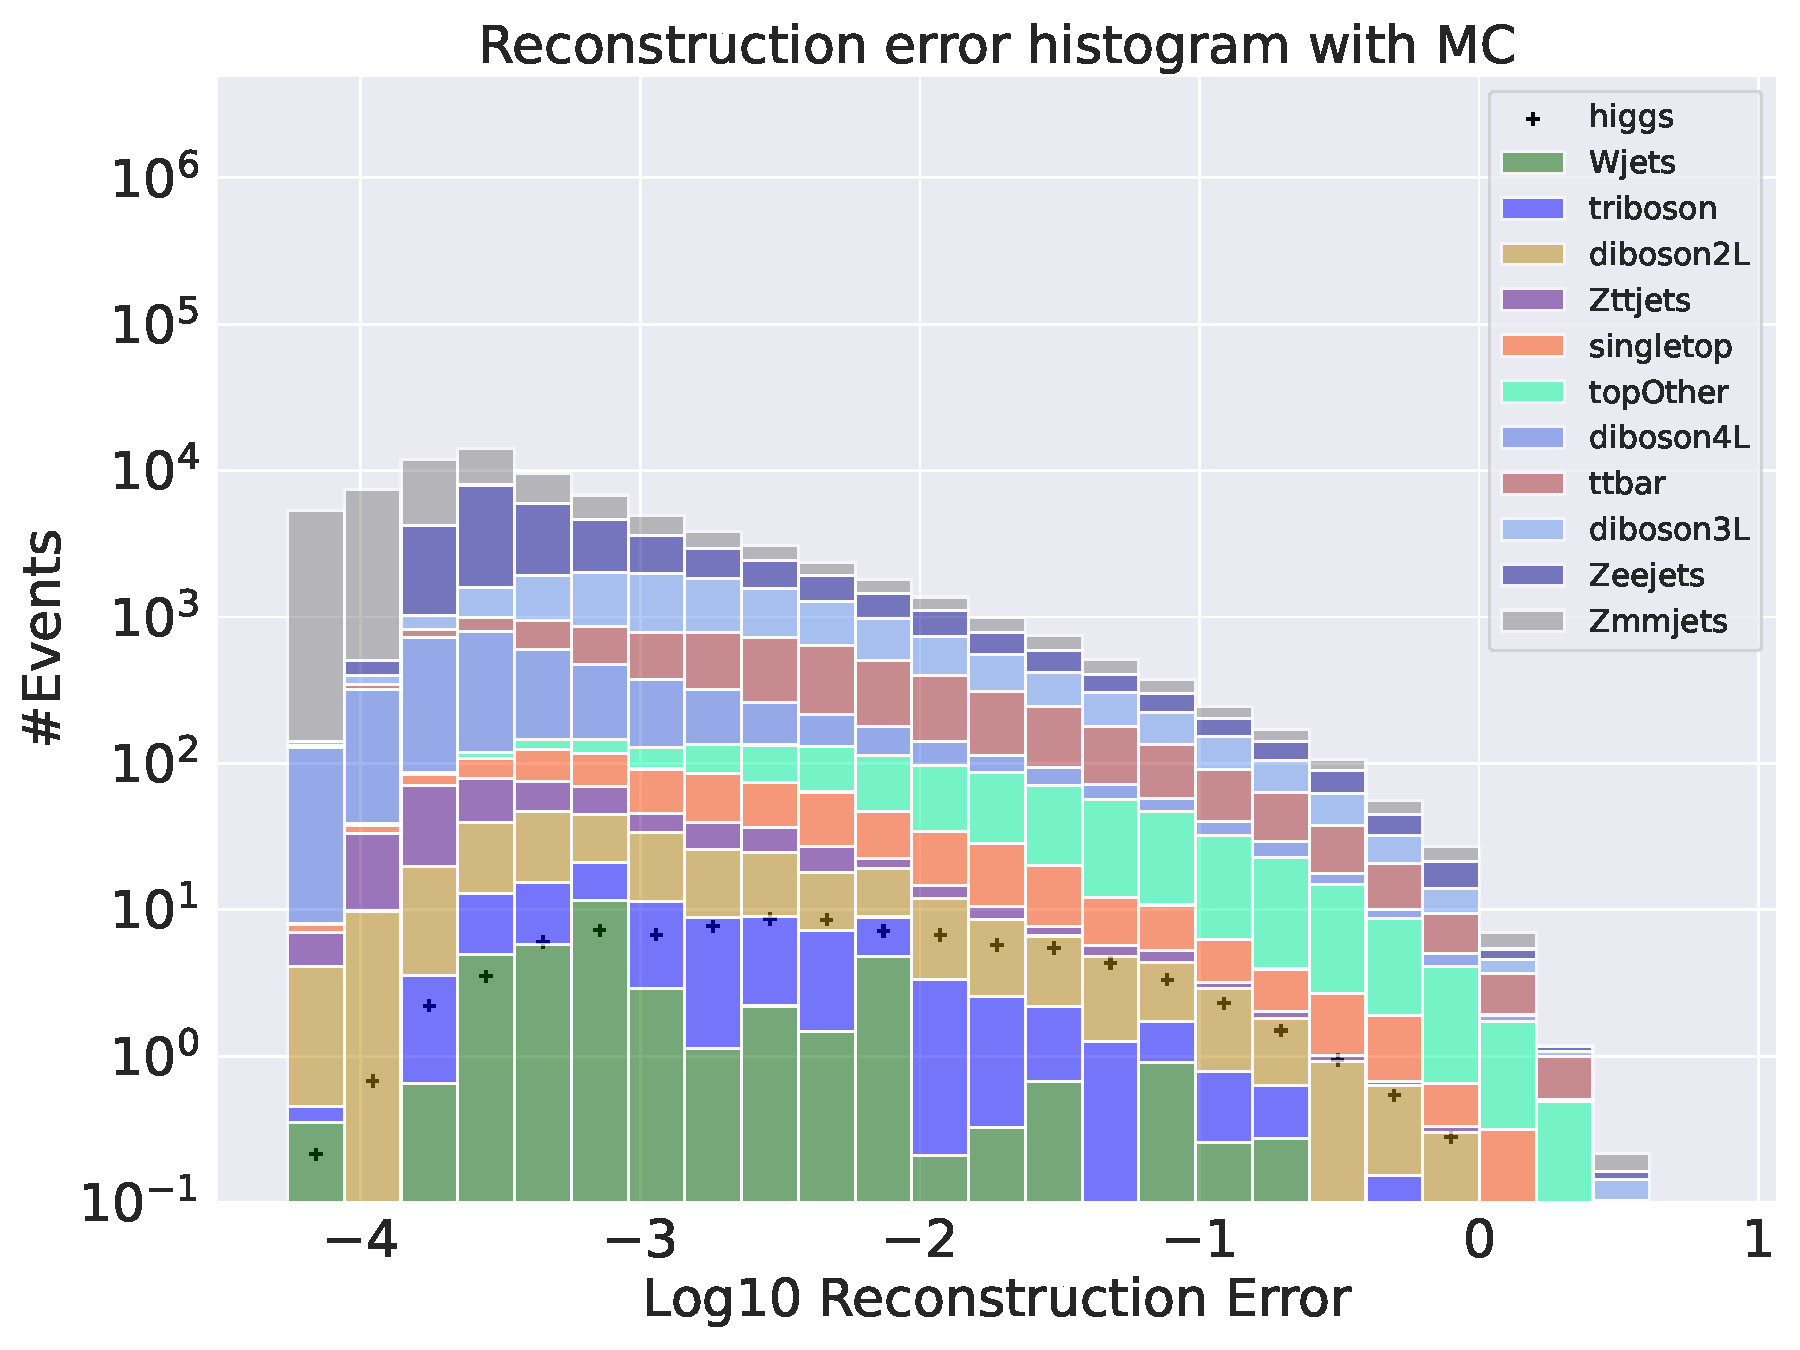
\includegraphics[width=\textwidth]{Figures/AE_testing/small/b_data_recon_big_rm3_feats_sig_higgs.pdf}
        \caption{Reconstruction error on validation SM MC from the small Autoencoder. Here the higgs channel has been removed from training and 
        is used as signal. No significant difference in distributions are found.}
        \label{fig:ae_small_higgs}
    \end{subfigure}
    \hfill 
    \begin{subfigure}{.45\textwidth}
        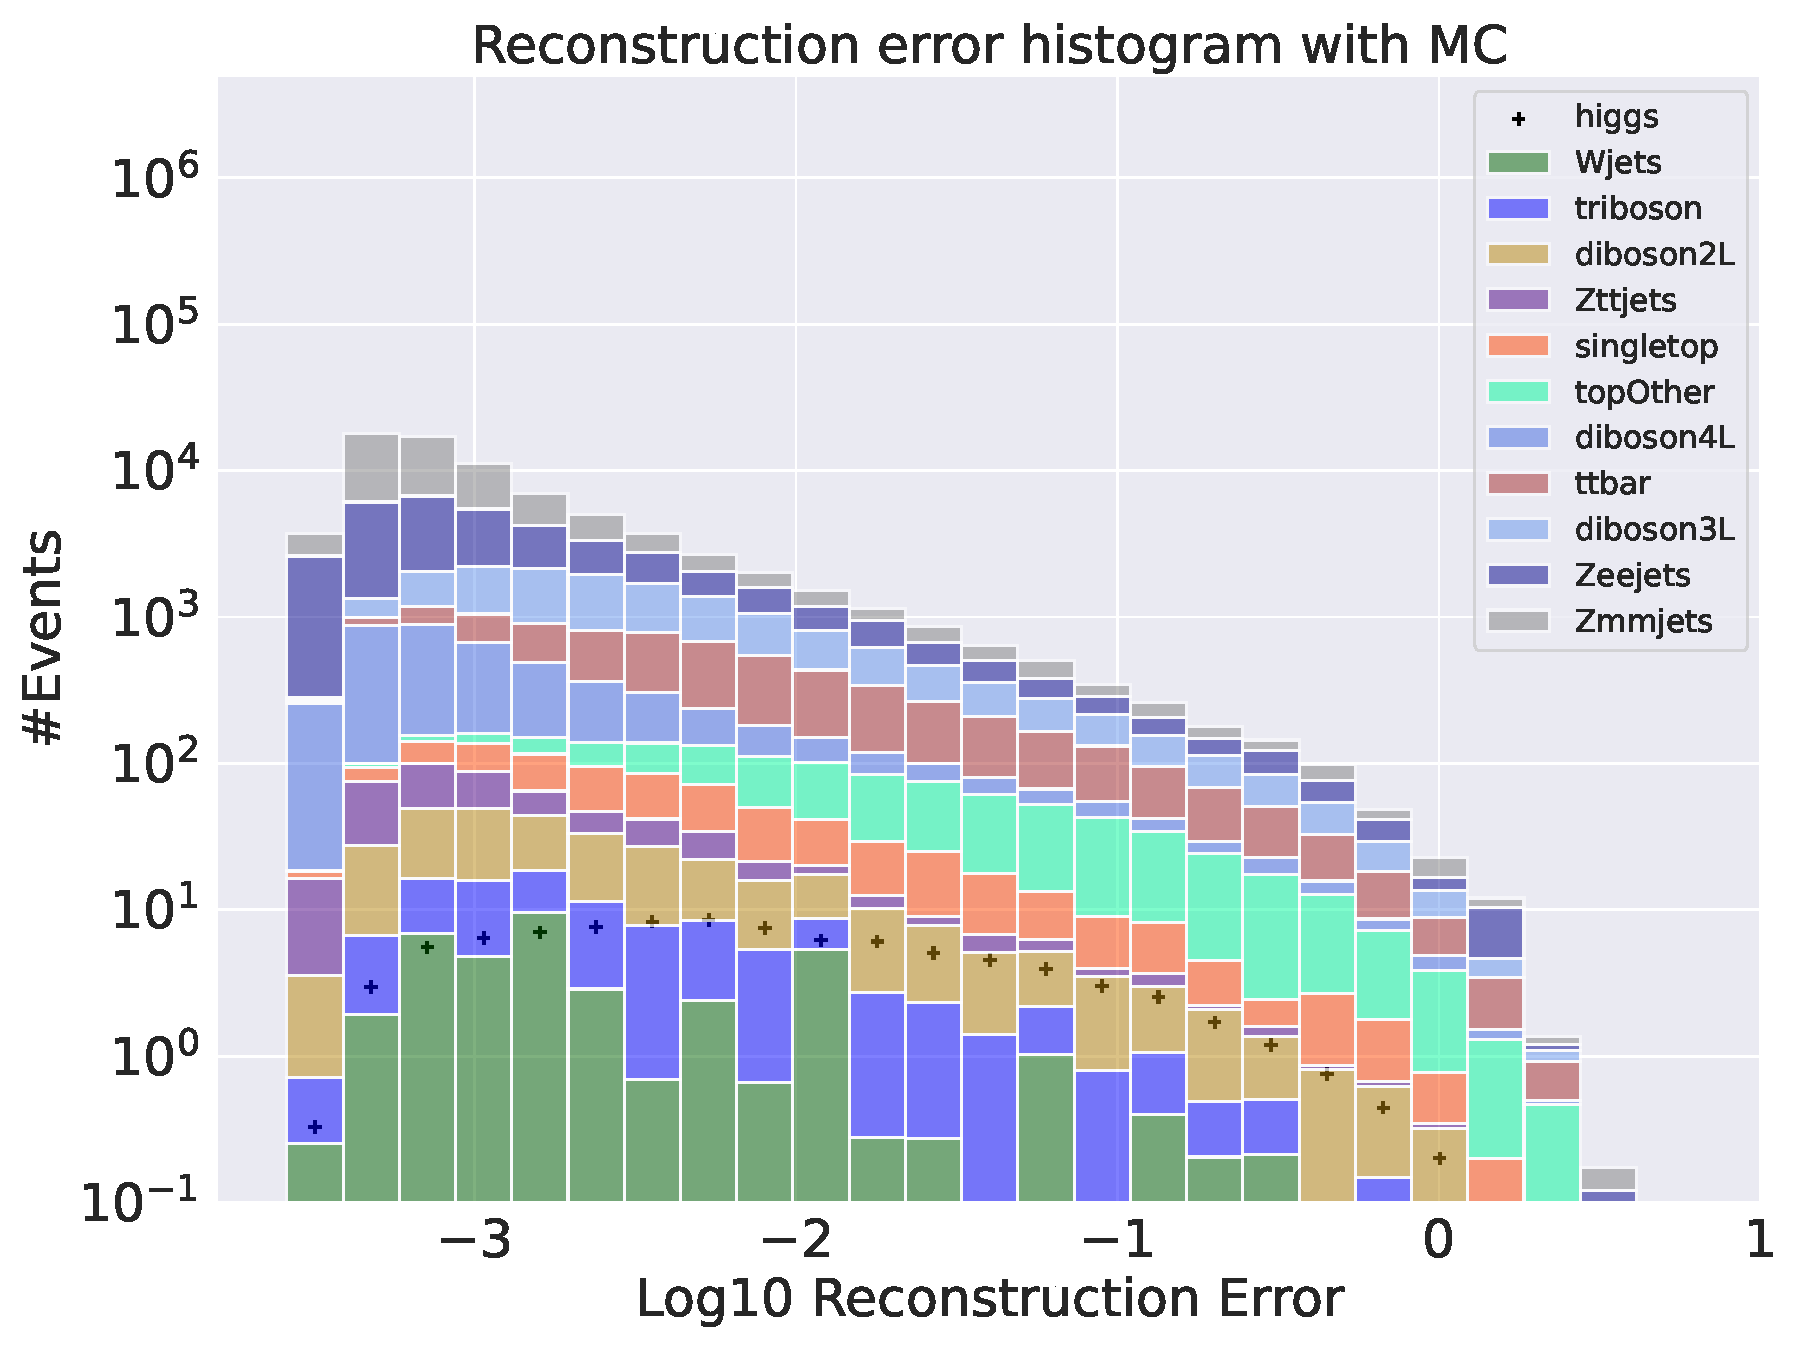
\includegraphics[width=\textwidth]{Figures/AE_testing/big/b_data_recon_big_rm3_feats_sig_higgs.pdf}
        \caption{Reconstruction error on validation SM MC from the big Autoencoder. Here the higgs channel has been removed from training and 
        is used as signal. No significant difference in distributions are found. }
        \label{fig:ae_big_higgs}
    \end{subfigure}
    \hfill 
    \caption[Reconstruction error using Higgs channel as signal]{Reconstruction error distributions for the small (to the left) and large (to the right) autoencoder using the Higgs channel as a signal, and 
    training the autoencoder on the remaining channels.  } 
    \label{fig:ae_big_channel_1}
    
\end{figure}

\begin{figure}[h!]
    \centering
    \begin{subfigure}{.45\textwidth}
        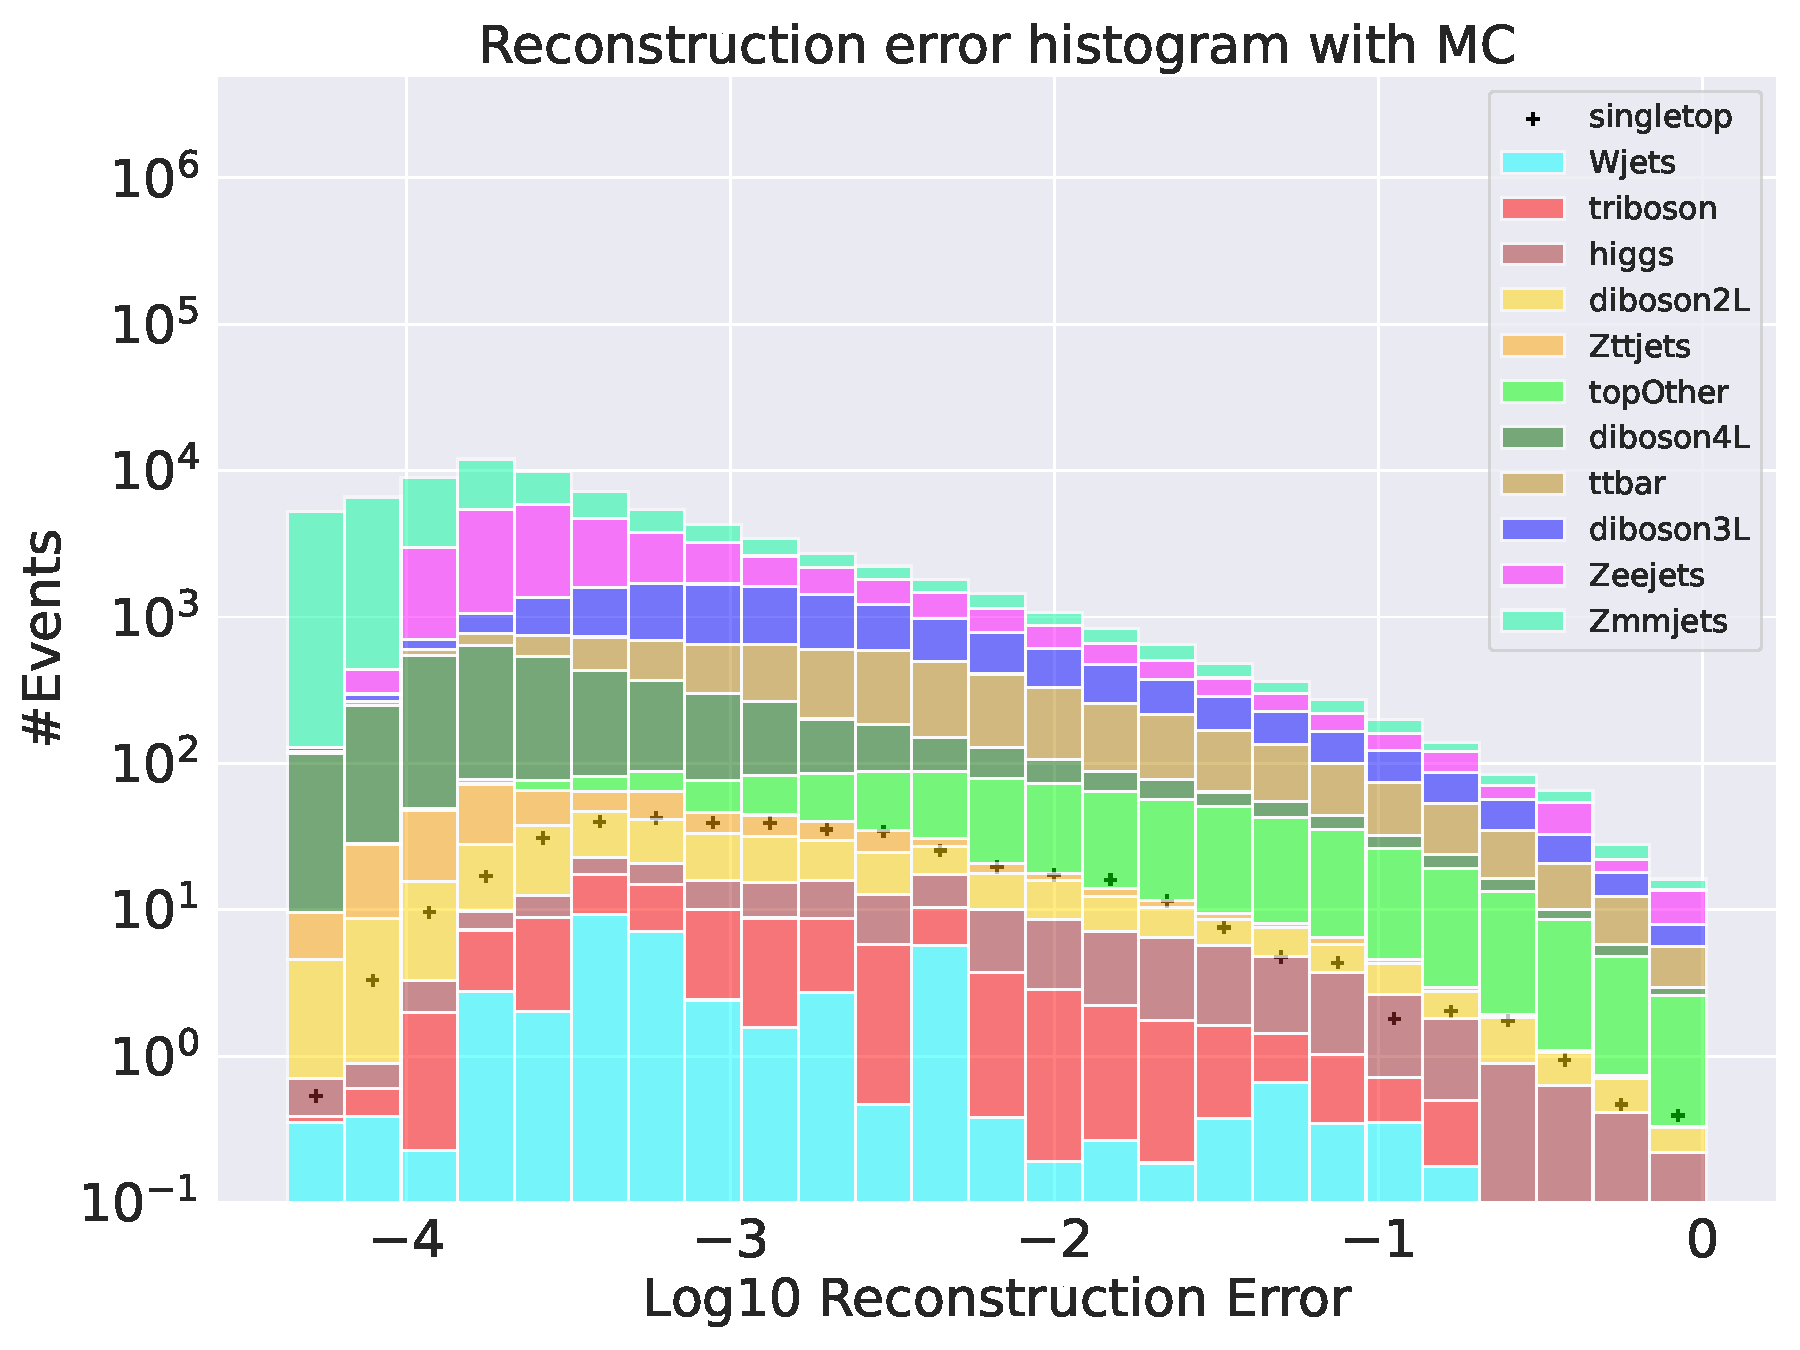
\includegraphics[width=\textwidth]{Figures/AE_testing/small/b_data_recon_big_rm3_feats_sig_singletop.pdf}
        \caption{Reconstruction error on validation SM MC from the small Autoencoder. Here the singletop channel has been removed from training and 
        is used as signal. No significant difference in distributions are found. }
        \label{fig:ae_small_singletop}
    \end{subfigure}
    \hfill
    \begin{subfigure}{.45\textwidth}
        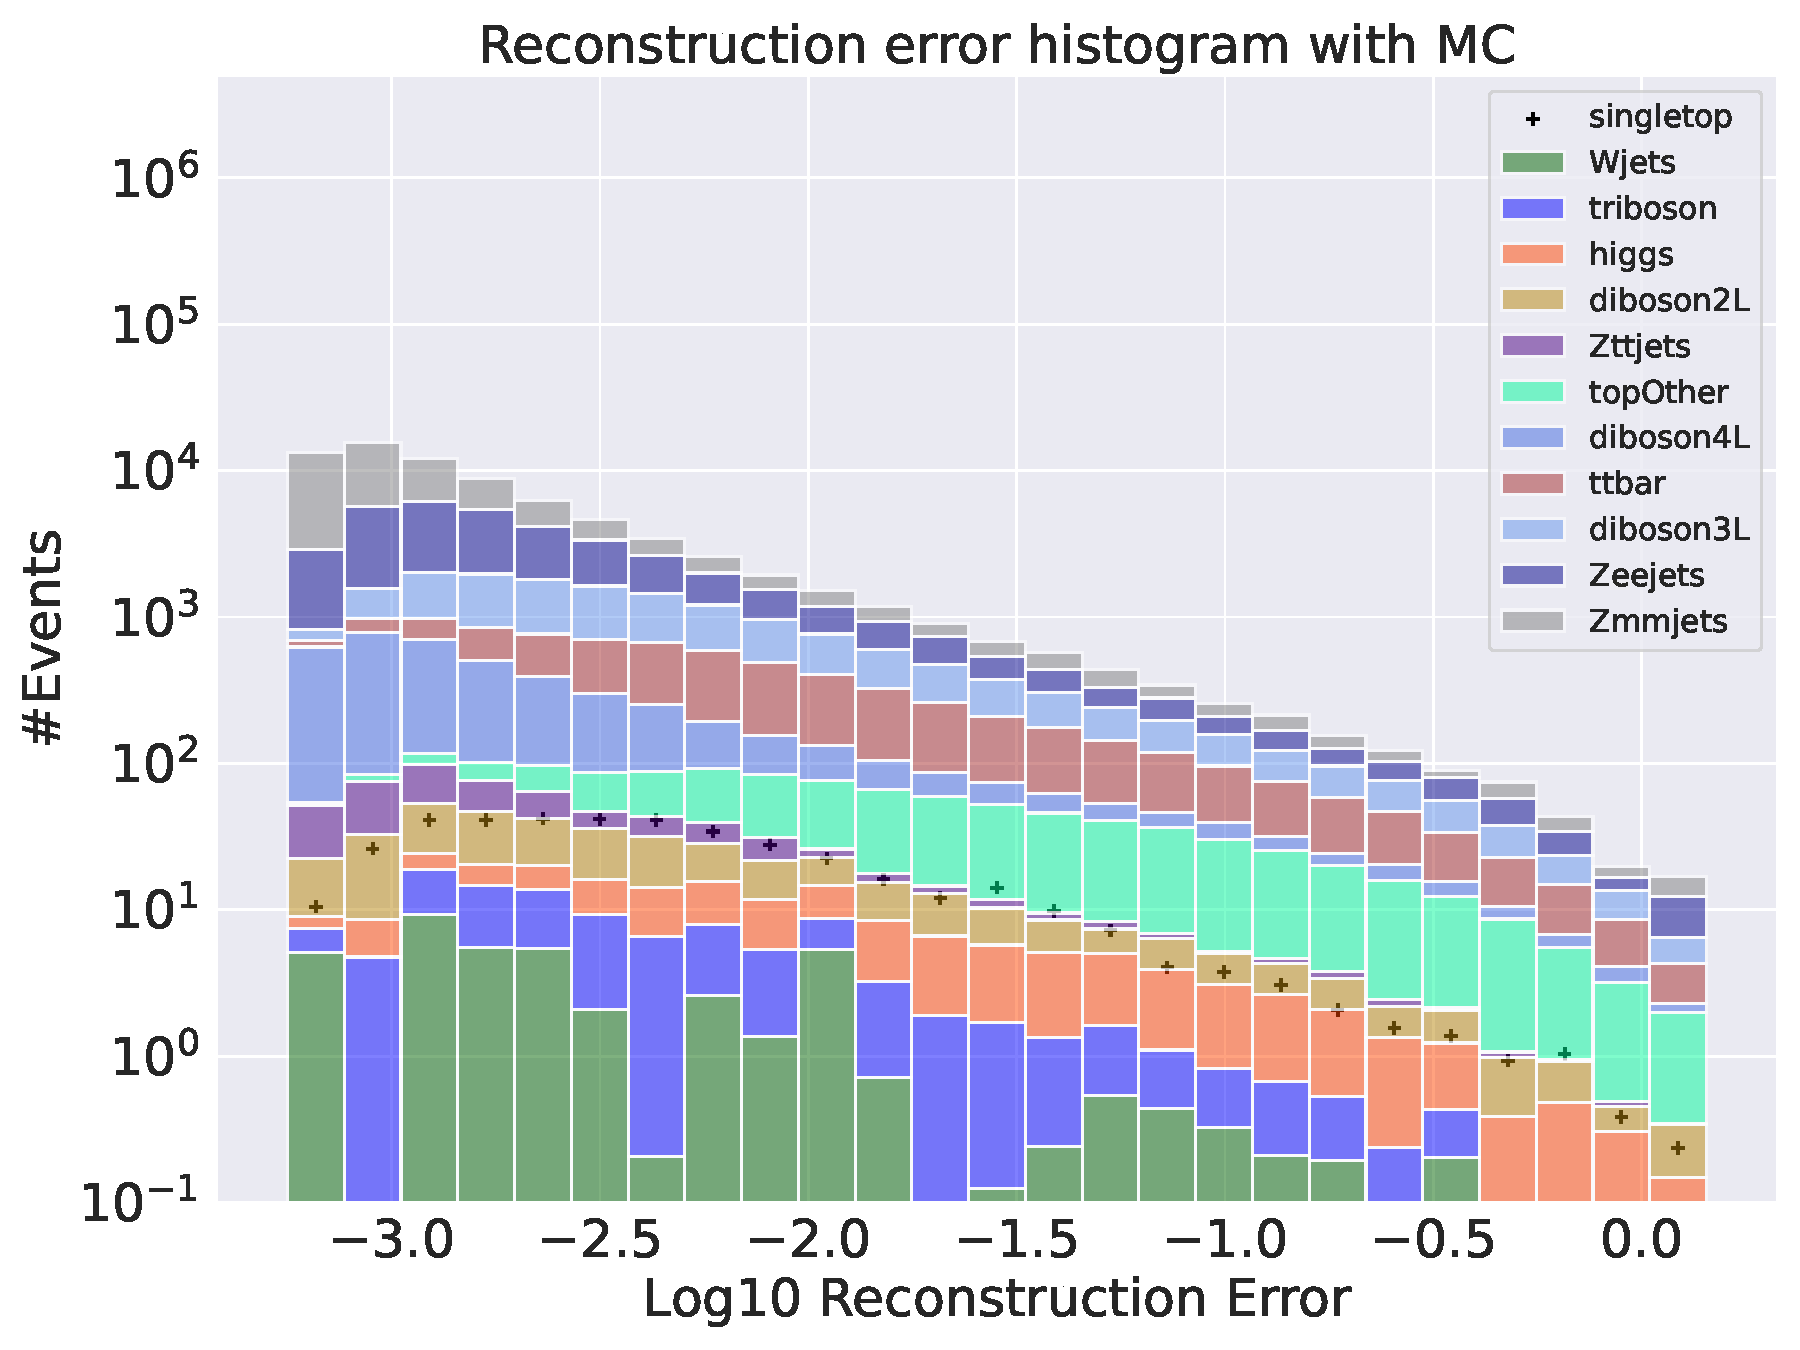
\includegraphics[width=\textwidth]{Figures/AE_testing/big/b_data_recon_big_rm3_feats_sig_singletop.pdf}
        \caption{Reconstruction error on validation SM MC from the big Autoencoder. Here the singletop channel has been removed from training and 
        is used as signal. No significant difference in distributions are found. }
        \label{fig:ae_big_singletop}
    \end{subfigure}
    \hfill
    \caption[Reconstruction error using Singletop channel as signal]{Reconstruction error distributions for the small (to the left) and large (to the right) autoencoder using the Singletop channel as a signal, and 
    training the autoencoder on the remaining channels. } 
    \label{fig:ae_big_channel_2}
\end{figure}

\begin{figure}[h!]
    \centering
    \begin{subfigure}{.45\textwidth}
        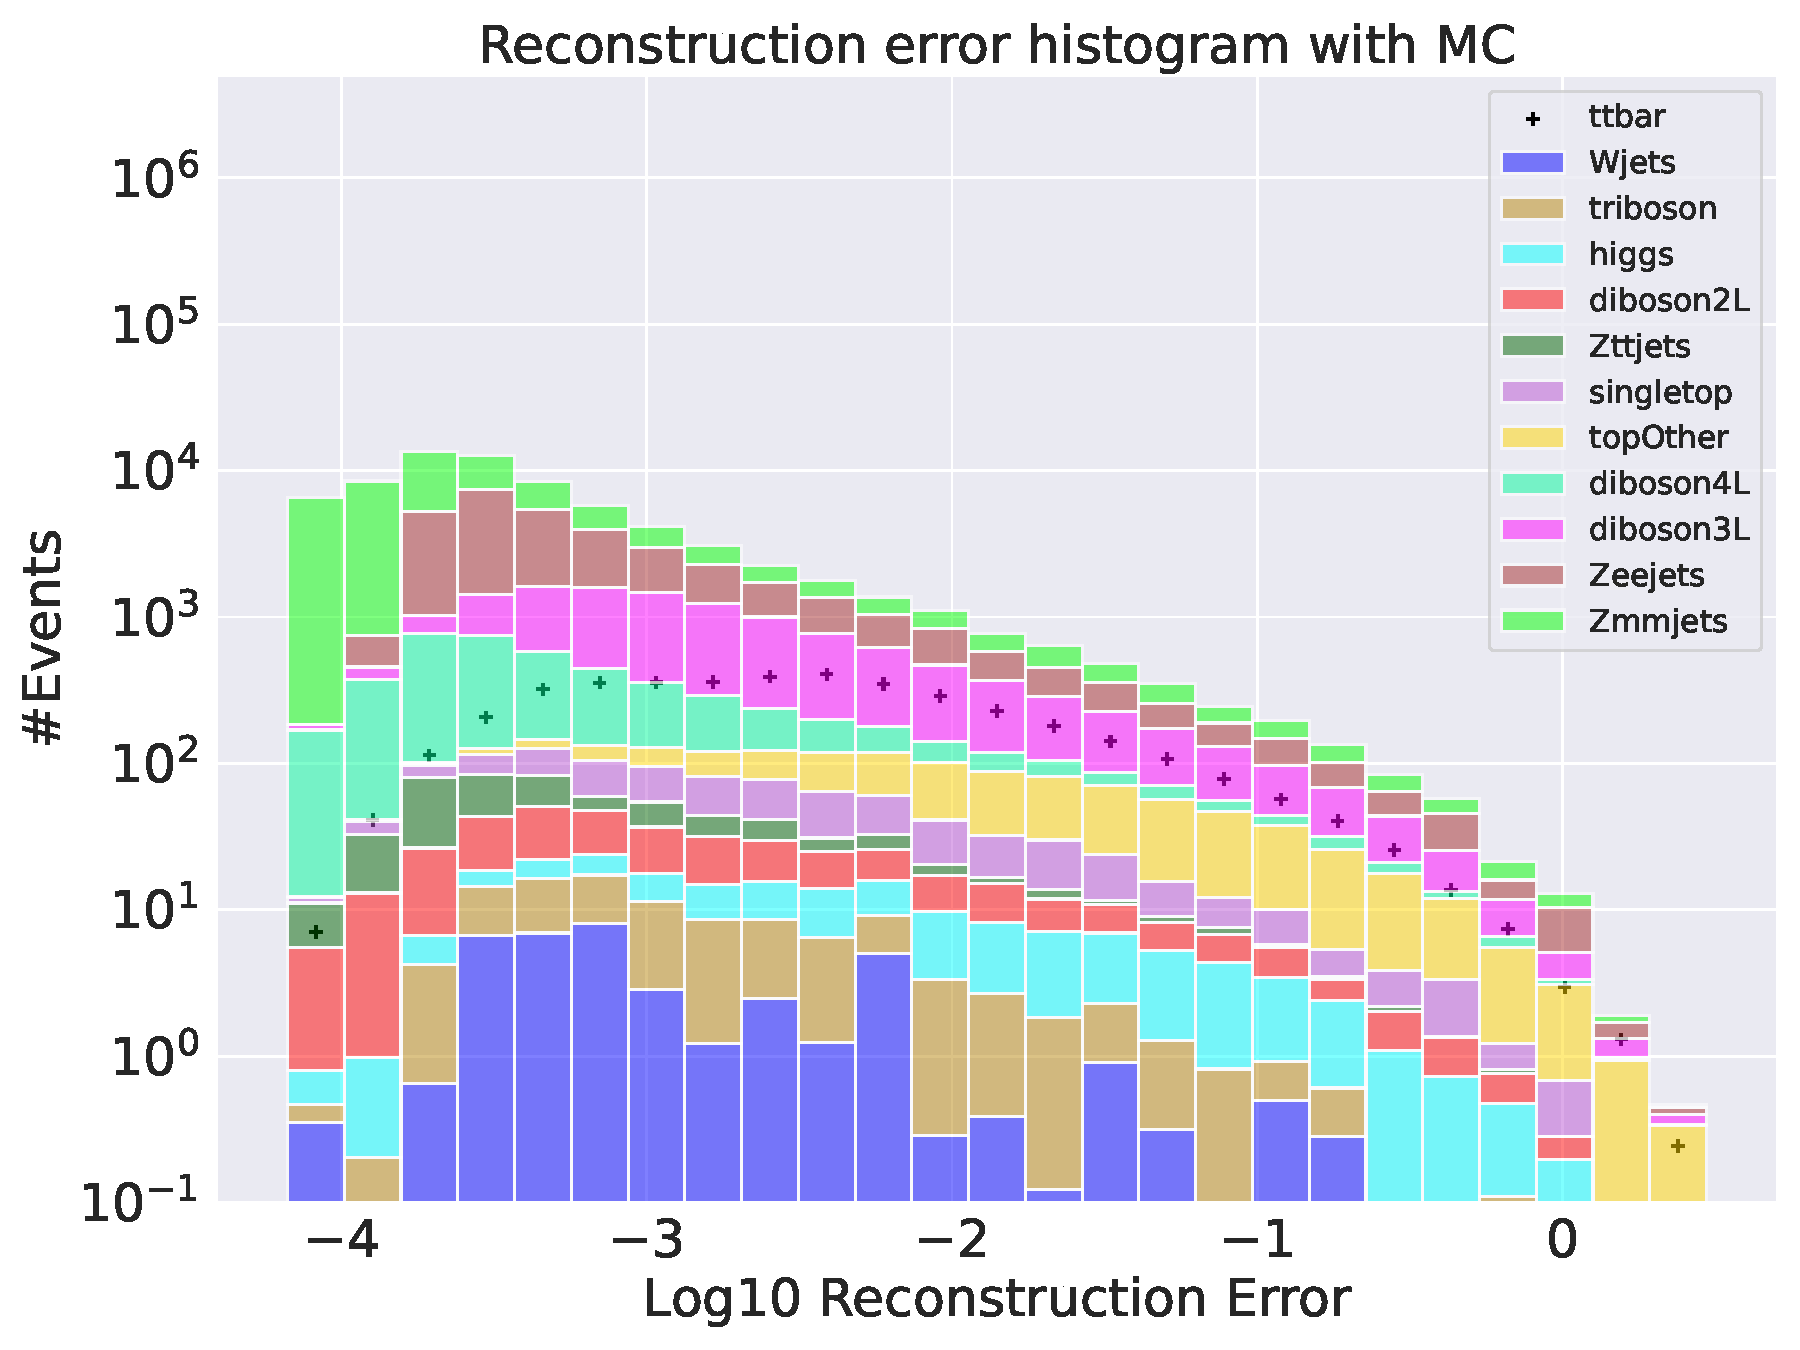
\includegraphics[width=\textwidth]{Figures/AE_testing/small/b_data_recon_big_rm3_feats_sig_ttbar.pdf}
        \caption{Reconstruction error on validation SM MC from the small Autoencoder. Here the ttbar channel has been removed from training and 
        is used as signal. No significant difference in distributions are found. }
        \label{fig:ae_small_ttbar}
    \end{subfigure}
    \hfill 
    \begin{subfigure}{.45\textwidth}
        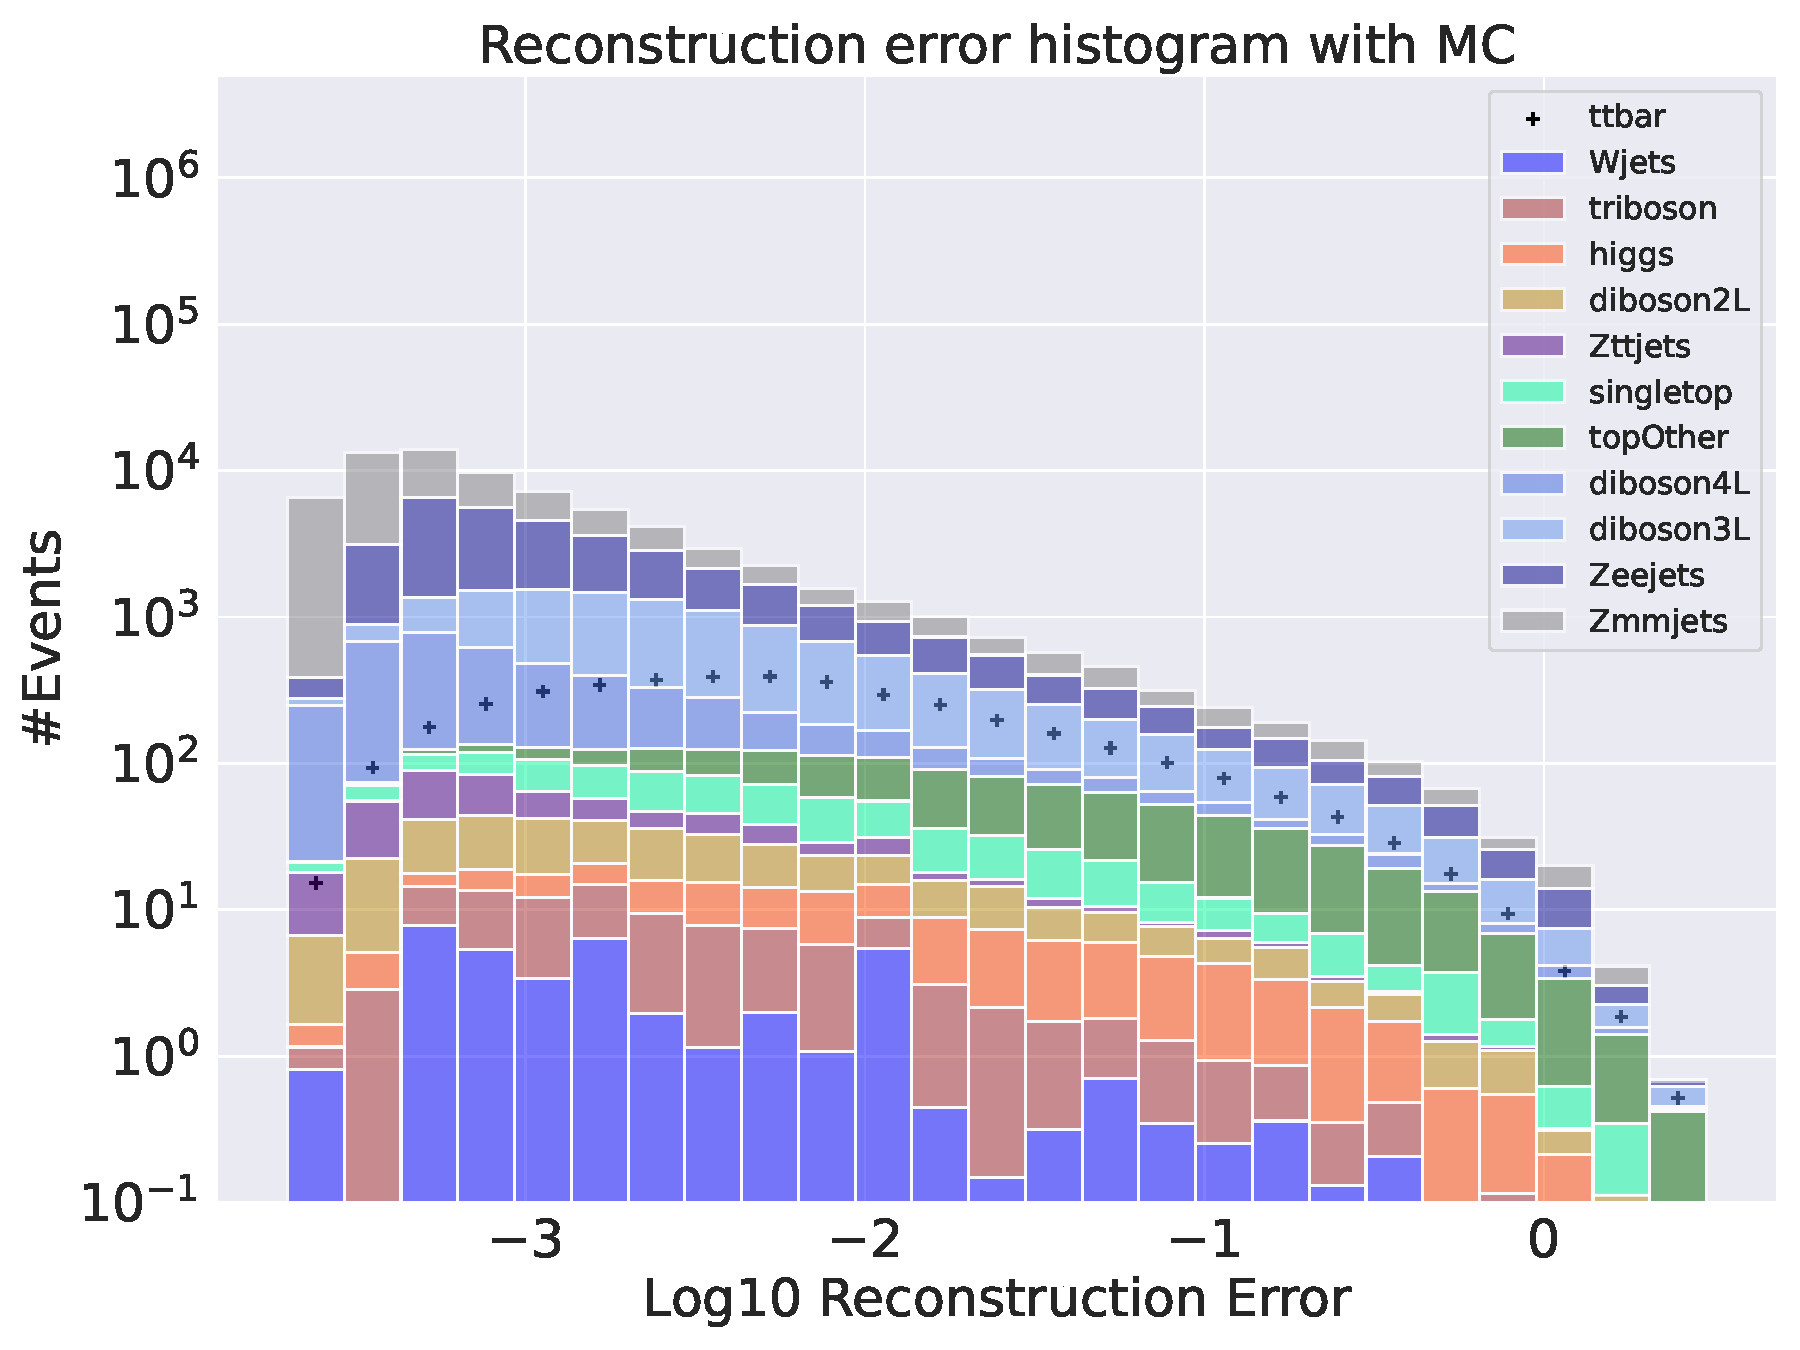
\includegraphics[width=\textwidth]{Figures/AE_testing/big/b_data_recon_big_rm3_feats_sig_ttbar.pdf}
        \caption{Reconstruction error on validation SM MC from the big Autoencoder. Here the ttbar channel has been removed from training and 
        is used as signal. No significant difference in distributions are found. }
        \label{fig:ae_big_ttbar}
    \end{subfigure}
    \hfill 
    \caption[Reconstruction error using ttbar channel as signal]{Reconstruction error distributions for the small (to the left) and large (to the right) autoencoder using the ttbar channel as a signal, and 
    training the autoencoder on the remaining channels. }
    \label[Reconstruction error using ttbar channel as signal]{fig:ae_big_channel_3}
\end{figure}



\begin{figure}[h!]
    \centering
    \begin{subfigure}{.45\textwidth}
        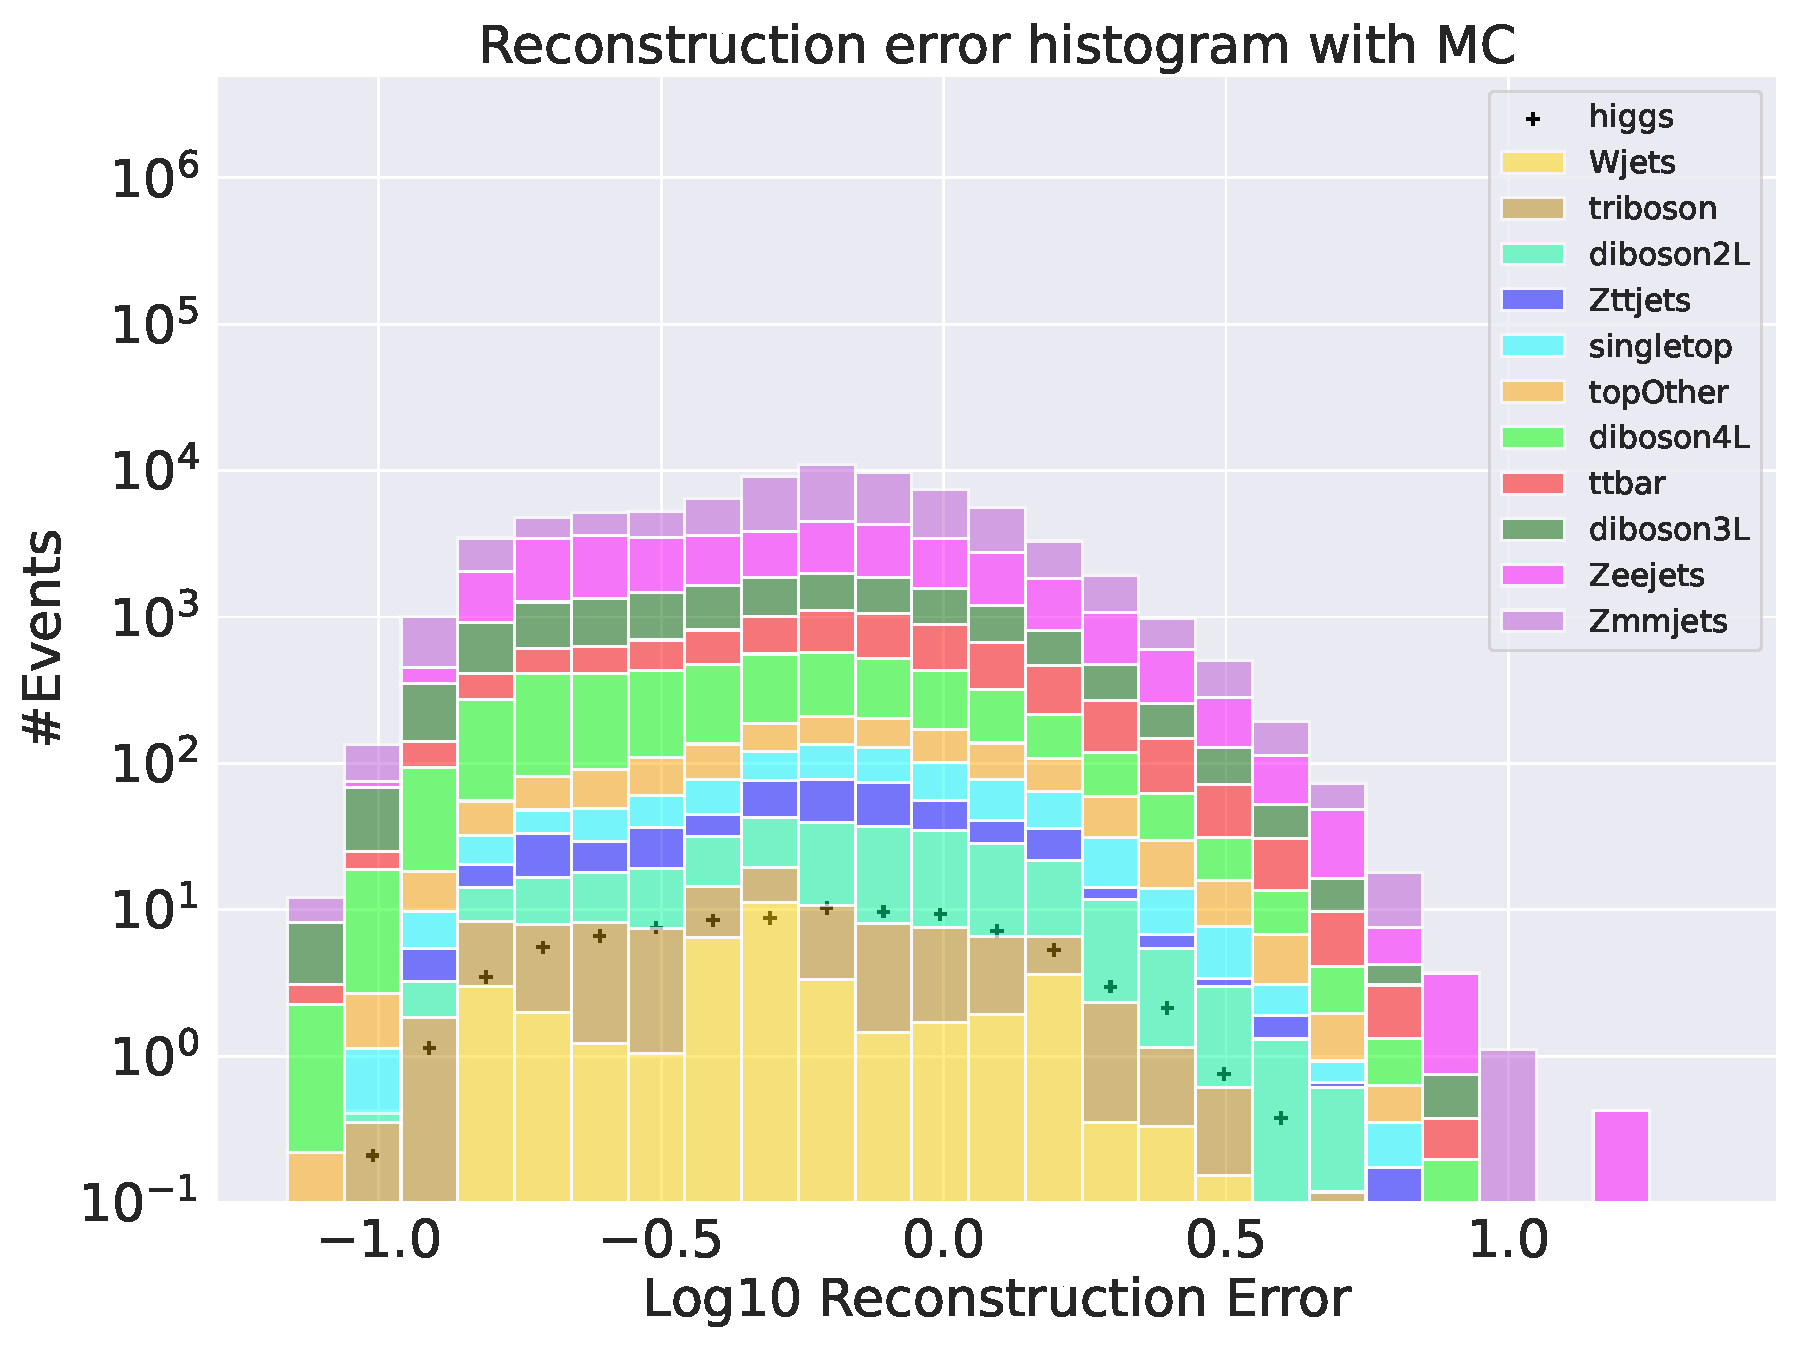
\includegraphics[width=\textwidth]{Figures/VAE_testing/small/b_data_recon_big_rm3_feats_sig_higgs.pdf}
        \caption{Reconstruction error on validation SM MC from the small variational Autoencoder. Here the higgs channel has been removed from training and 
        is used as signal. No significant difference in distributions are found.}
        \label{fig:vae_small_higgs}
    \end{subfigure}
    \hfill 
    \begin{subfigure}{.45\textwidth}
        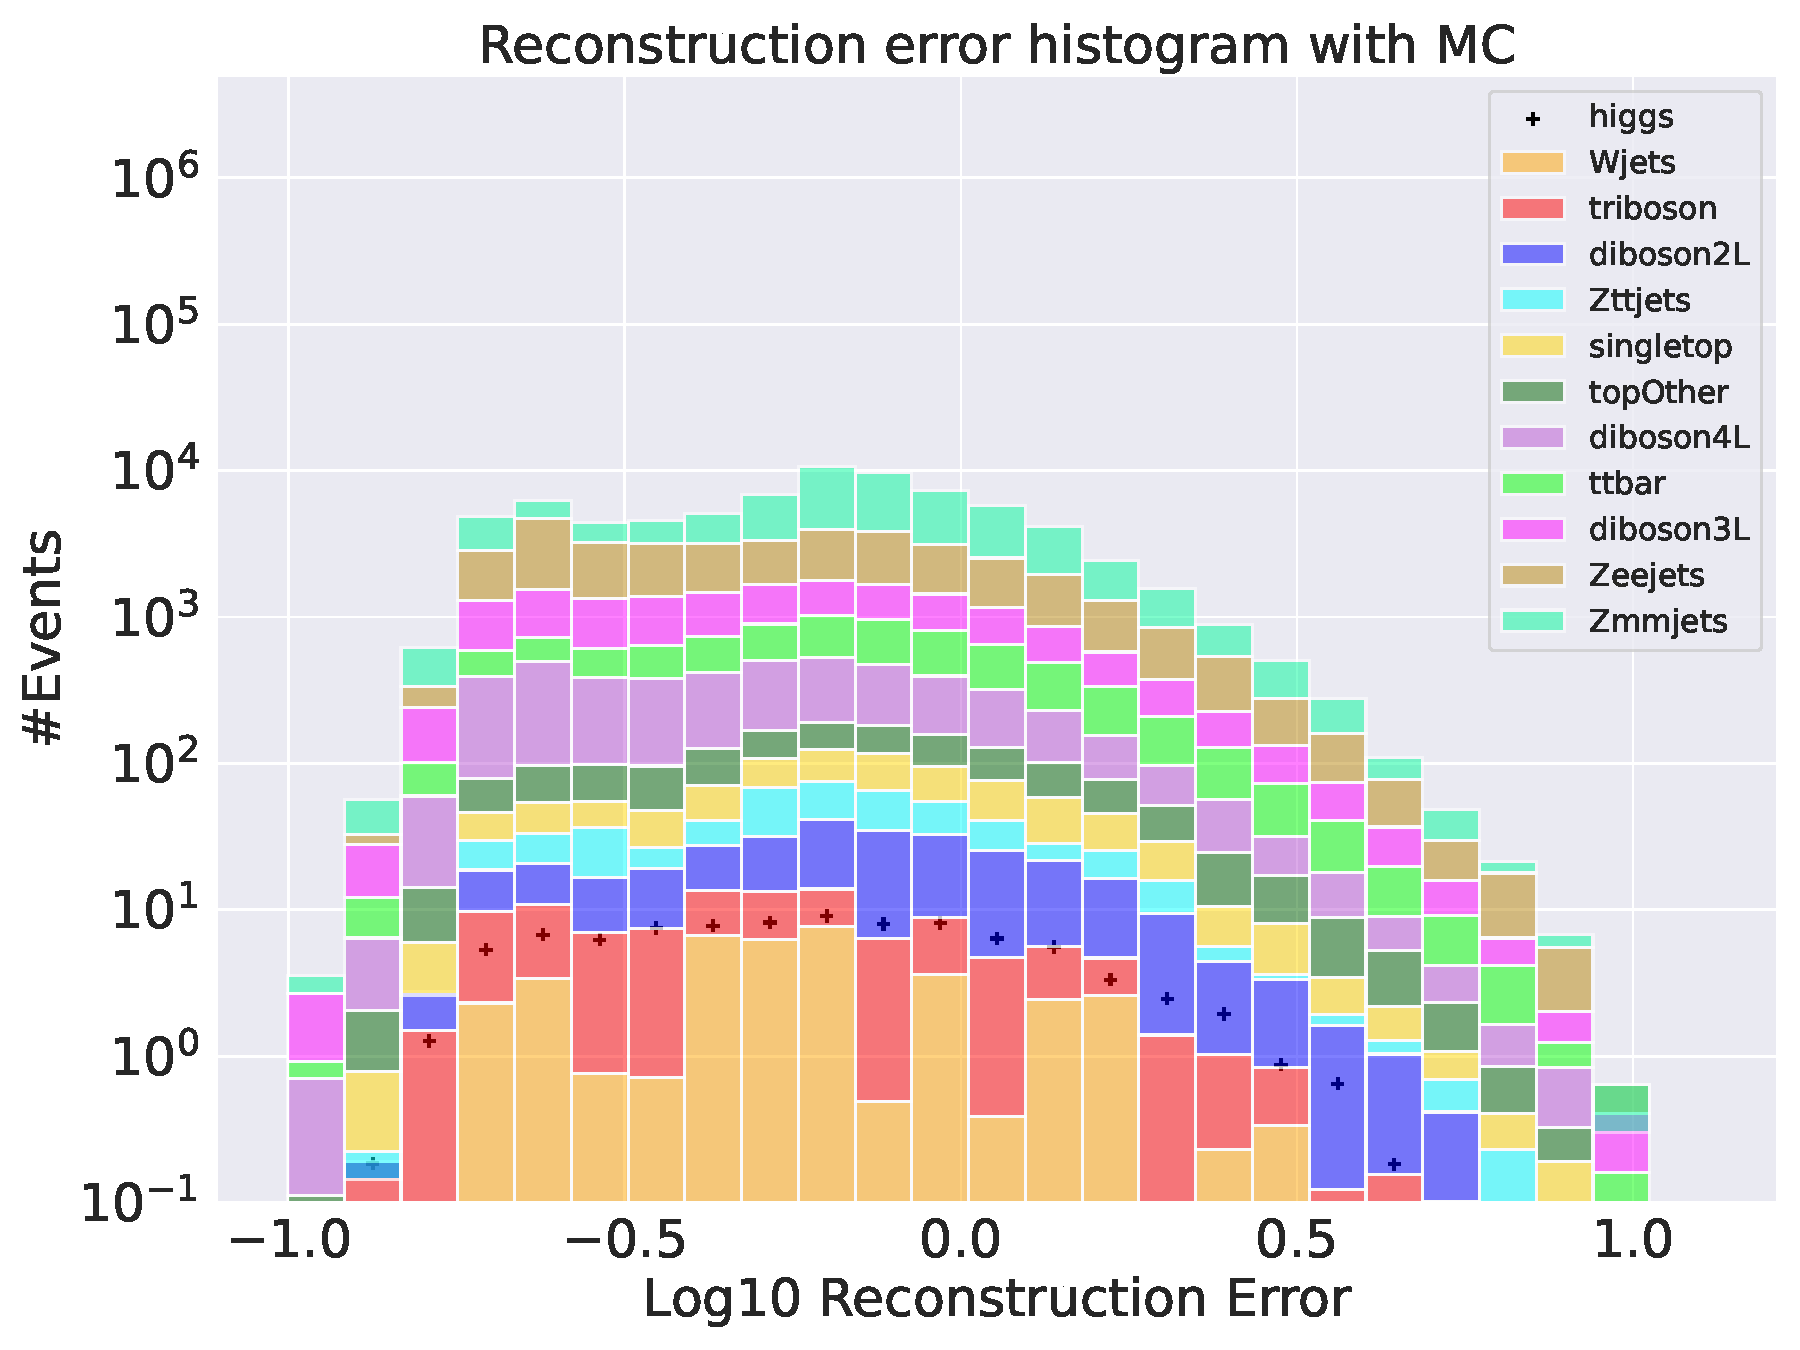
\includegraphics[width=\textwidth]{Figures/VAE_testing/big/b_data_recon_big_rm3_feats_sig_higgs.pdf}
        \caption{Reconstruction error on validation SM MC from the big variational Autoencoder. Here the higgs channel has been removed from training and 
        is used as signal. No significant difference in distributions are found. }
        \label{fig:vae_big_higgs}
    \end{subfigure}
    \hfill  
    \caption[Reconstruction error using Higgs channel as signal]{Reconstruction error distributions for the small (to the left) and large (to the right) autoencoder using the Higgs channel as a signal, and 
    training the autoencoder on the remaining channels. }
    \label{fig:vae_big_channel_1}
\end{figure}

\begin{figure}[h!]
    \centering
    \begin{subfigure}{.45\textwidth}
        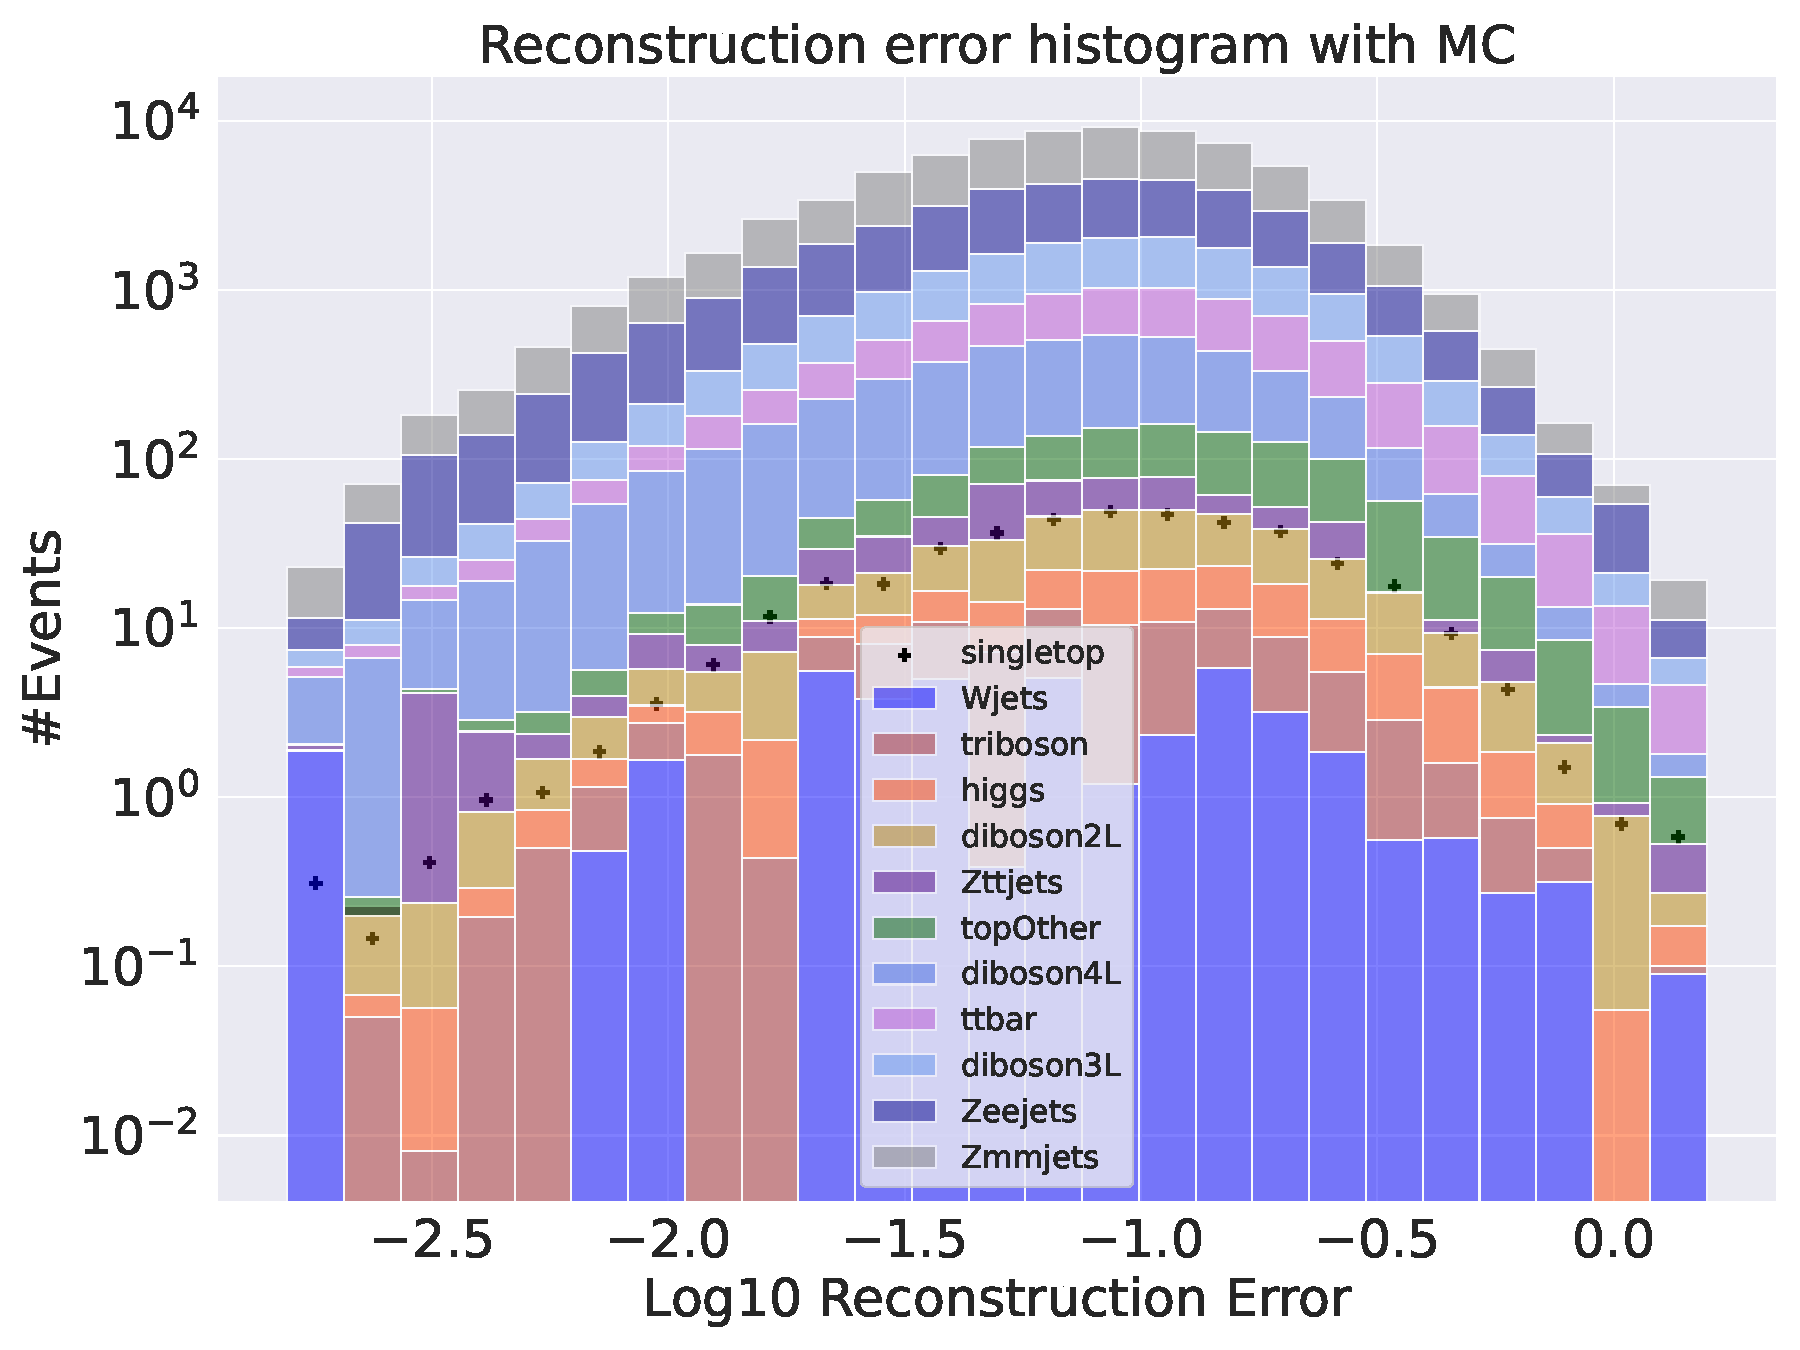
\includegraphics[width=\textwidth]{Figures/VAE_testing/small/b_data_recon_big_rm3_feats_sig_singletop.pdf}
        \caption{Reconstruction error on validation SM MC from the small variational Autoencoder. Here the singletop channel has been removed from training and 
        is used as signal. No significant difference in distributions are found. }
        \label{fig:vae_small_singletop}
    \end{subfigure}
    \hfill
    \begin{subfigure}{.45\textwidth}
        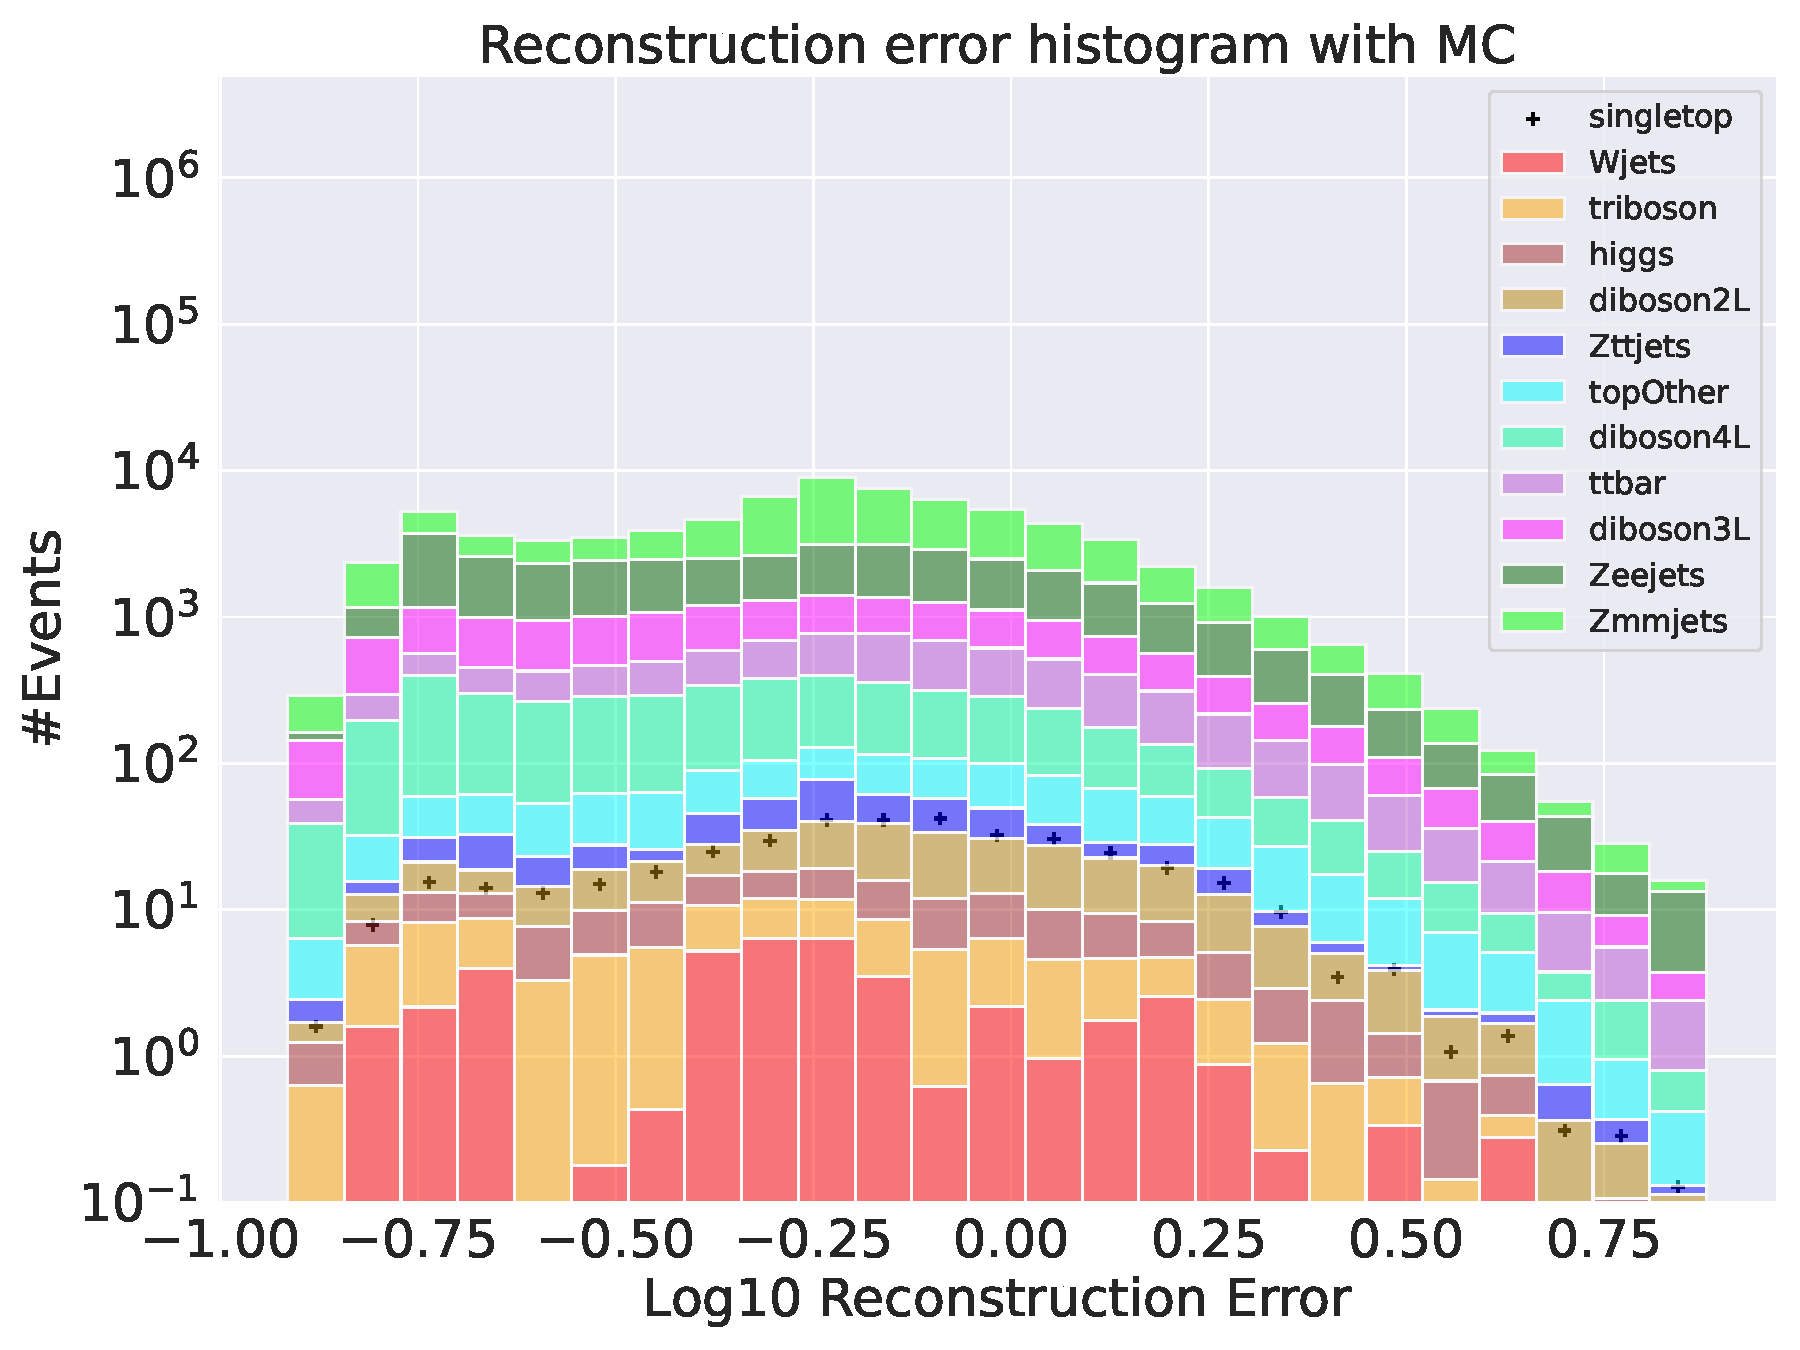
\includegraphics[width=\textwidth]{Figures/VAE_testing/big/b_data_recon_big_rm3_feats_sig_singletop.pdf}
        \caption{Reconstruction error on validation SM MC from the big variational Autoencoder. Here the singletop channel has been removed from training and 
        is used as signal. No significant difference in distributions are found. }
        \label{fig:vae_big_singletop}
    \end{subfigure}
    \hfill 
    \caption[Reconstruction error using Singletop channel as signal]{Reconstruction error distributions for the small (to the left) and large (to the right) autoencoder using the Singletop channel as a signal, and 
    training the autoencoder on the remaining channels. }
    \label{fig:vae_big_channel_2}
\end{figure}

\begin{figure}[h!]
    \centering
    \begin{subfigure}{.45\textwidth}
        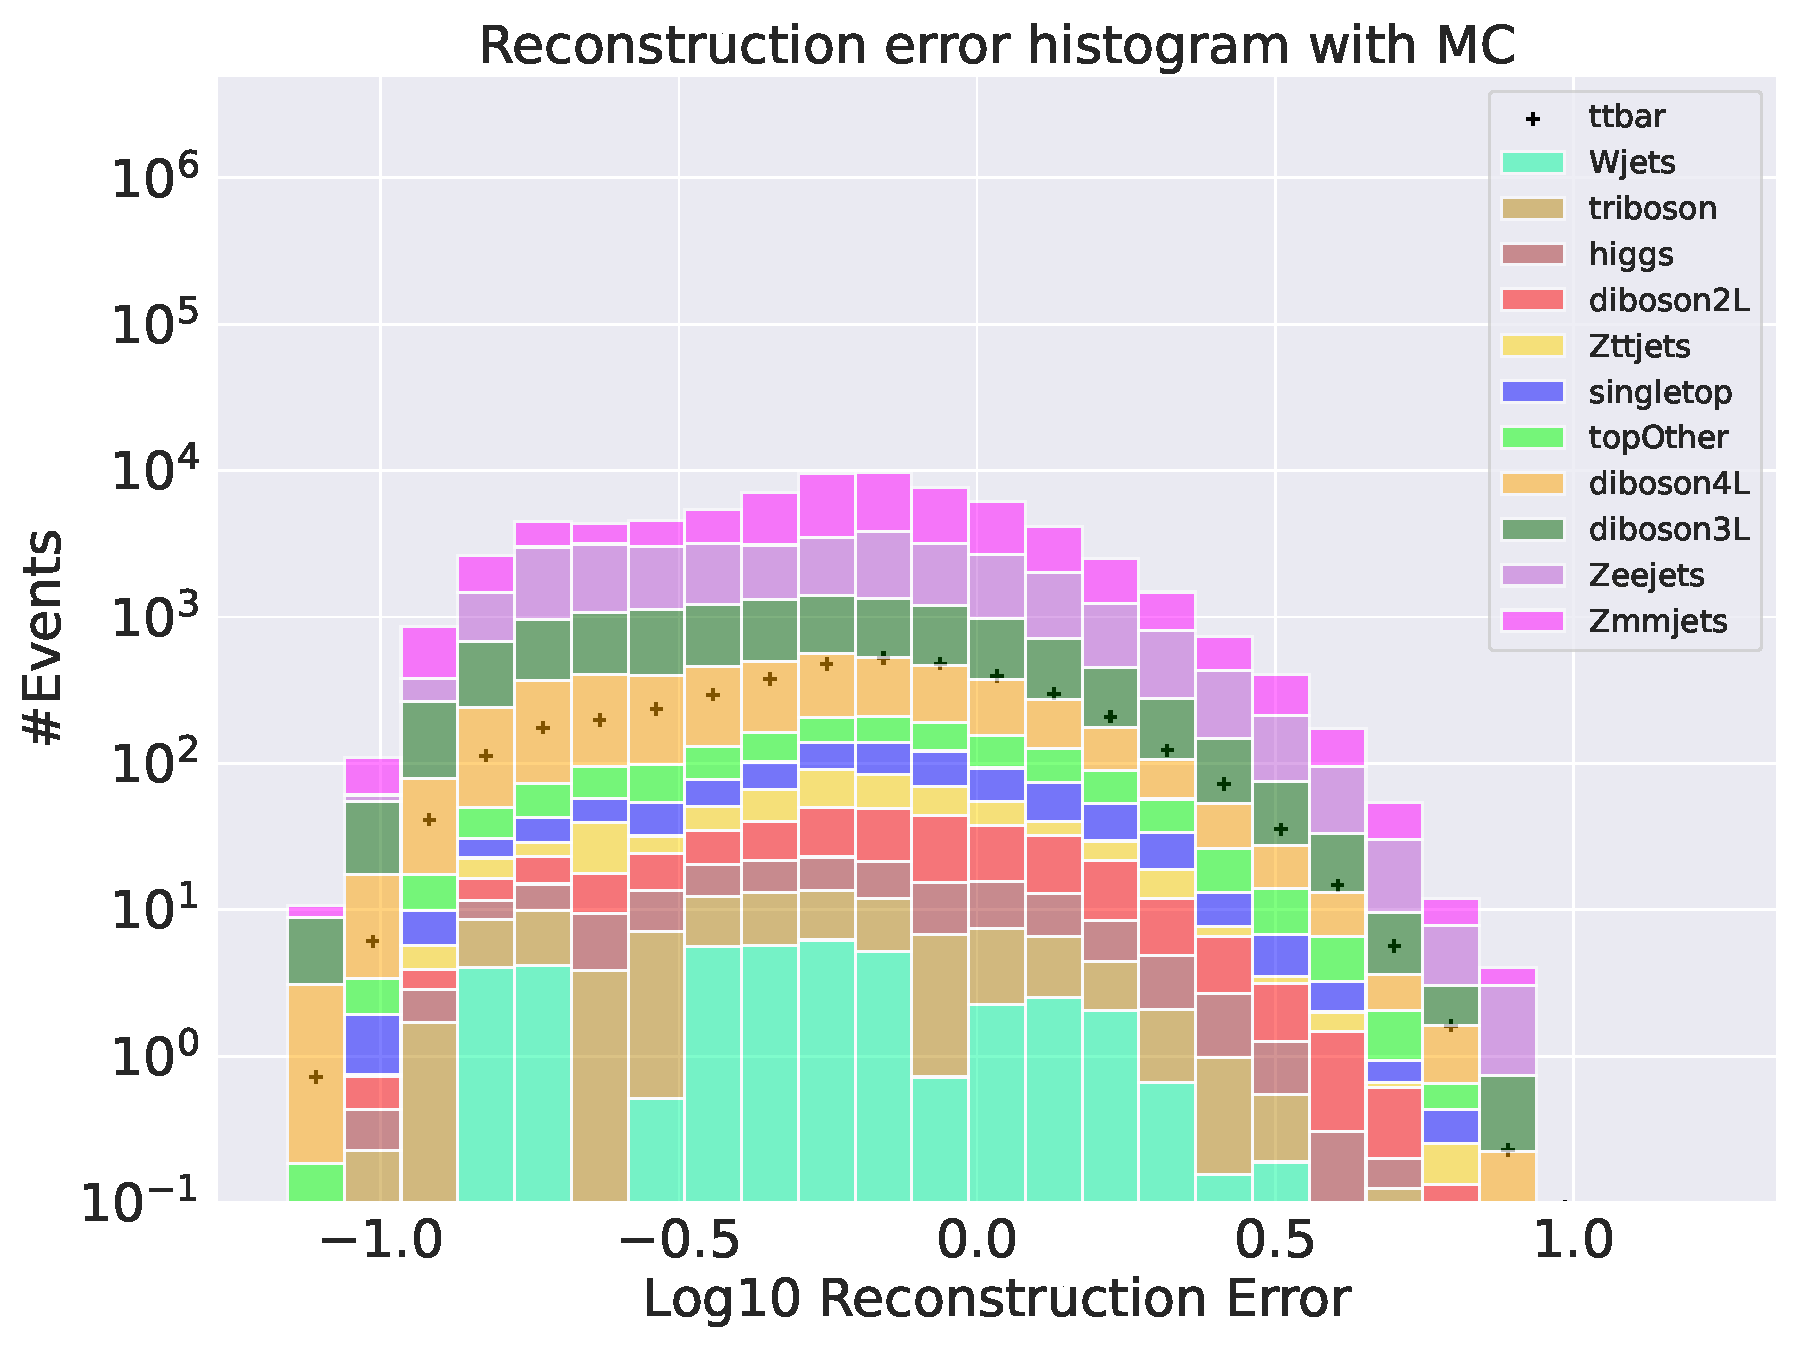
\includegraphics[width=\textwidth]{Figures/VAE_testing/small/b_data_recon_big_rm3_feats_sig_ttbar.pdf}
        \caption{Reconstruction error on validation SM MC from the small variational Autoencoder. Here the ttbar channel has been removed from training and 
        is used as signal. No significant difference in distributions are found. }
        \label{fig:vae_small_ttbar}
    \end{subfigure}
    \hfill 
    \begin{subfigure}{.45\textwidth}
        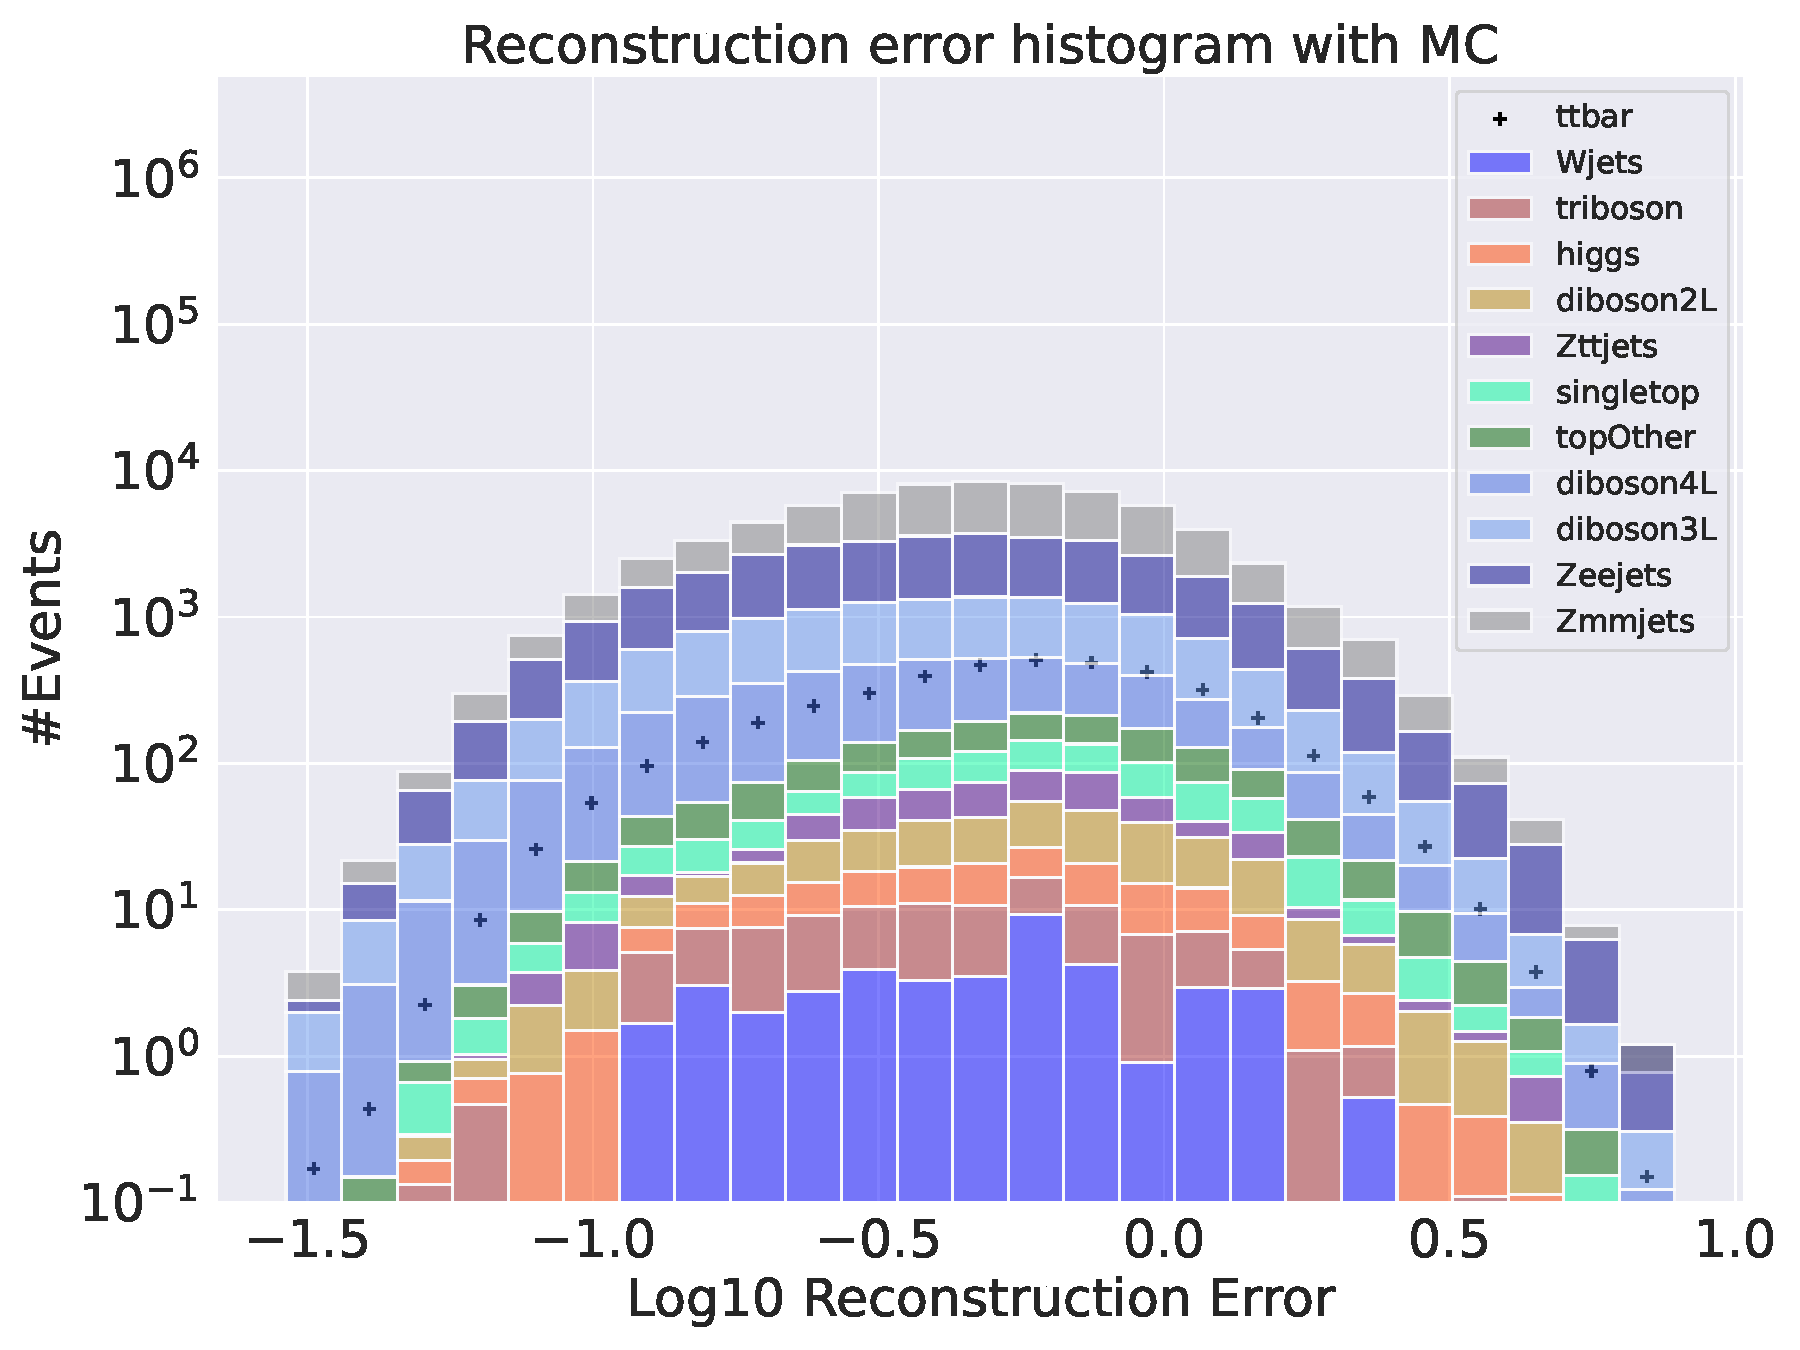
\includegraphics[width=\textwidth]{Figures/VAE_testing/big/b_data_recon_big_rm3_feats_sig_ttbar.pdf}
        \caption{Reconstruction error on validation SM MC from the big variational Autoencoder. Here the ttbar channel has been removed from training and 
        is used as signal. No significant difference in distributions are found. }
        \label{fig:vae_big_ttbar}
    \end{subfigure}
    \hfill 
    \caption[Reconstruction error using ttbar channel as signal]{Reconstruction error distributions for the small (to the left) and large (to the right) autoencoder using the ttbar channel as a signal, and 
    training the autoencoder on the remaining channels. }
    \label{fig:vae_big_channel_3}
\end{figure}

In figures \ref{fig:ae_big_channel_1} to \ref{fig:vae_big_channel_3} we have the reconstruction error distributions for the SM MC using 
Higgs, singletop and ttbar as signal samples for the small (to the left) and the big (to the right) regular and variational autoencoder. 
It is clear from figures that the reconstruction error distributions for the removed SM channel and the remainding SM MC are very similar. 
The same behavior is also shown for the other channels, which can found in appendix 2. All though the two models struggled to get a 
separation of reconstruction error distributions, the regular autoencoder seems to have a more shifted pattern of reconstruction to lower 
values than the variational autoencoder. In fact, the regular autoencoder's reconstruction error distribution peak is about 3 order of 
magnitude lower than the variational autoencoder's error distribution peak. There could be several reasons for this, one of which is that 
the variational autoencoder requires more input data to approximate the distribution, as well as the fact that the balance between the KL divergence and MSE loss 
can be difficult to handle\cite{kl_mse_balance}. This can lead to poor performance of the network. It should be notet that all though the 
three channels selected here, as well as the rest in appendix 2, do not differ that much from one another, and the hopes were not high that 
the networks would be able to separate the two distributions created. However it does provide us with a baseline, as well as insight for what 
to expect if we were to test on signals that looks a lot like some channels. 


\newpage


\subsection*{Altering of transverse momentum}
Altering the transverse momentum of some particles would in the extreme be anomalous and the hypothesis was that some of those trends would be
picked up by the autoencoder. Several scales for the transverse momentum were used, with the following results.

\subsubsection*{Autoencoder}

\begin{figure}[h!]
    \centering
    \begin{subfigure}{.45\textwidth}
        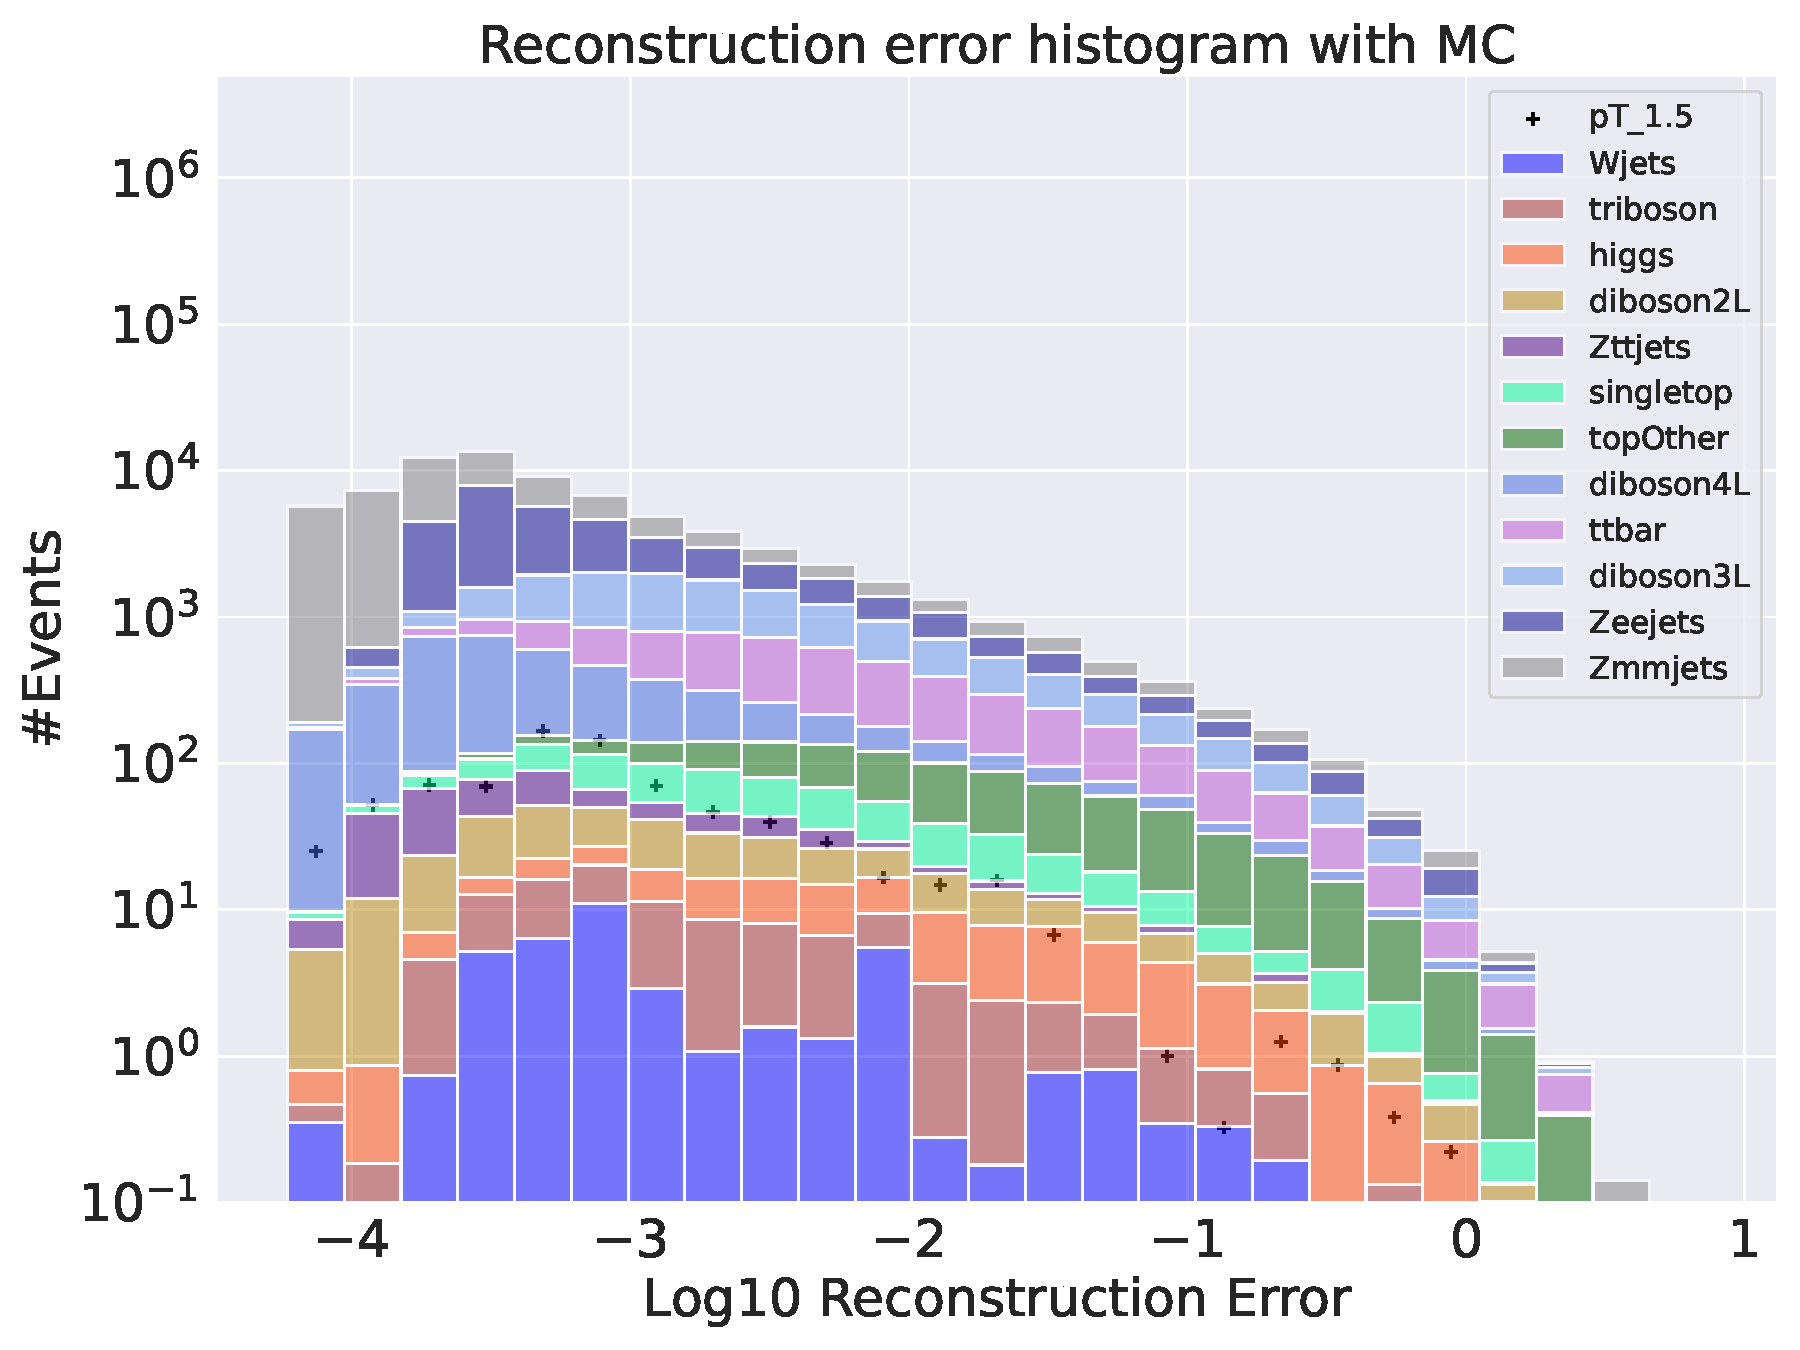
\includegraphics[width=\textwidth]{Figures/AE_testing/small/b_data_recon_big_rm3_feats_sig_pT_1.5.pdf}
        \caption{Reconstruction error on validation SM MC from the small variational Autoencoder. Here the signal is a subsample of the validation 
        set where the transverse momentum of the first electron and the first muon has been increased with a scale of $1.5$. The change of transverse 
        energy has thusly also been changed according to the scaling of transverse momentum. No significant difference in distributions are found. }
        \label{fig:ae_small_pt_1_5}
    \end{subfigure}
    \hfill 
    \begin{subfigure}{.45\textwidth}
        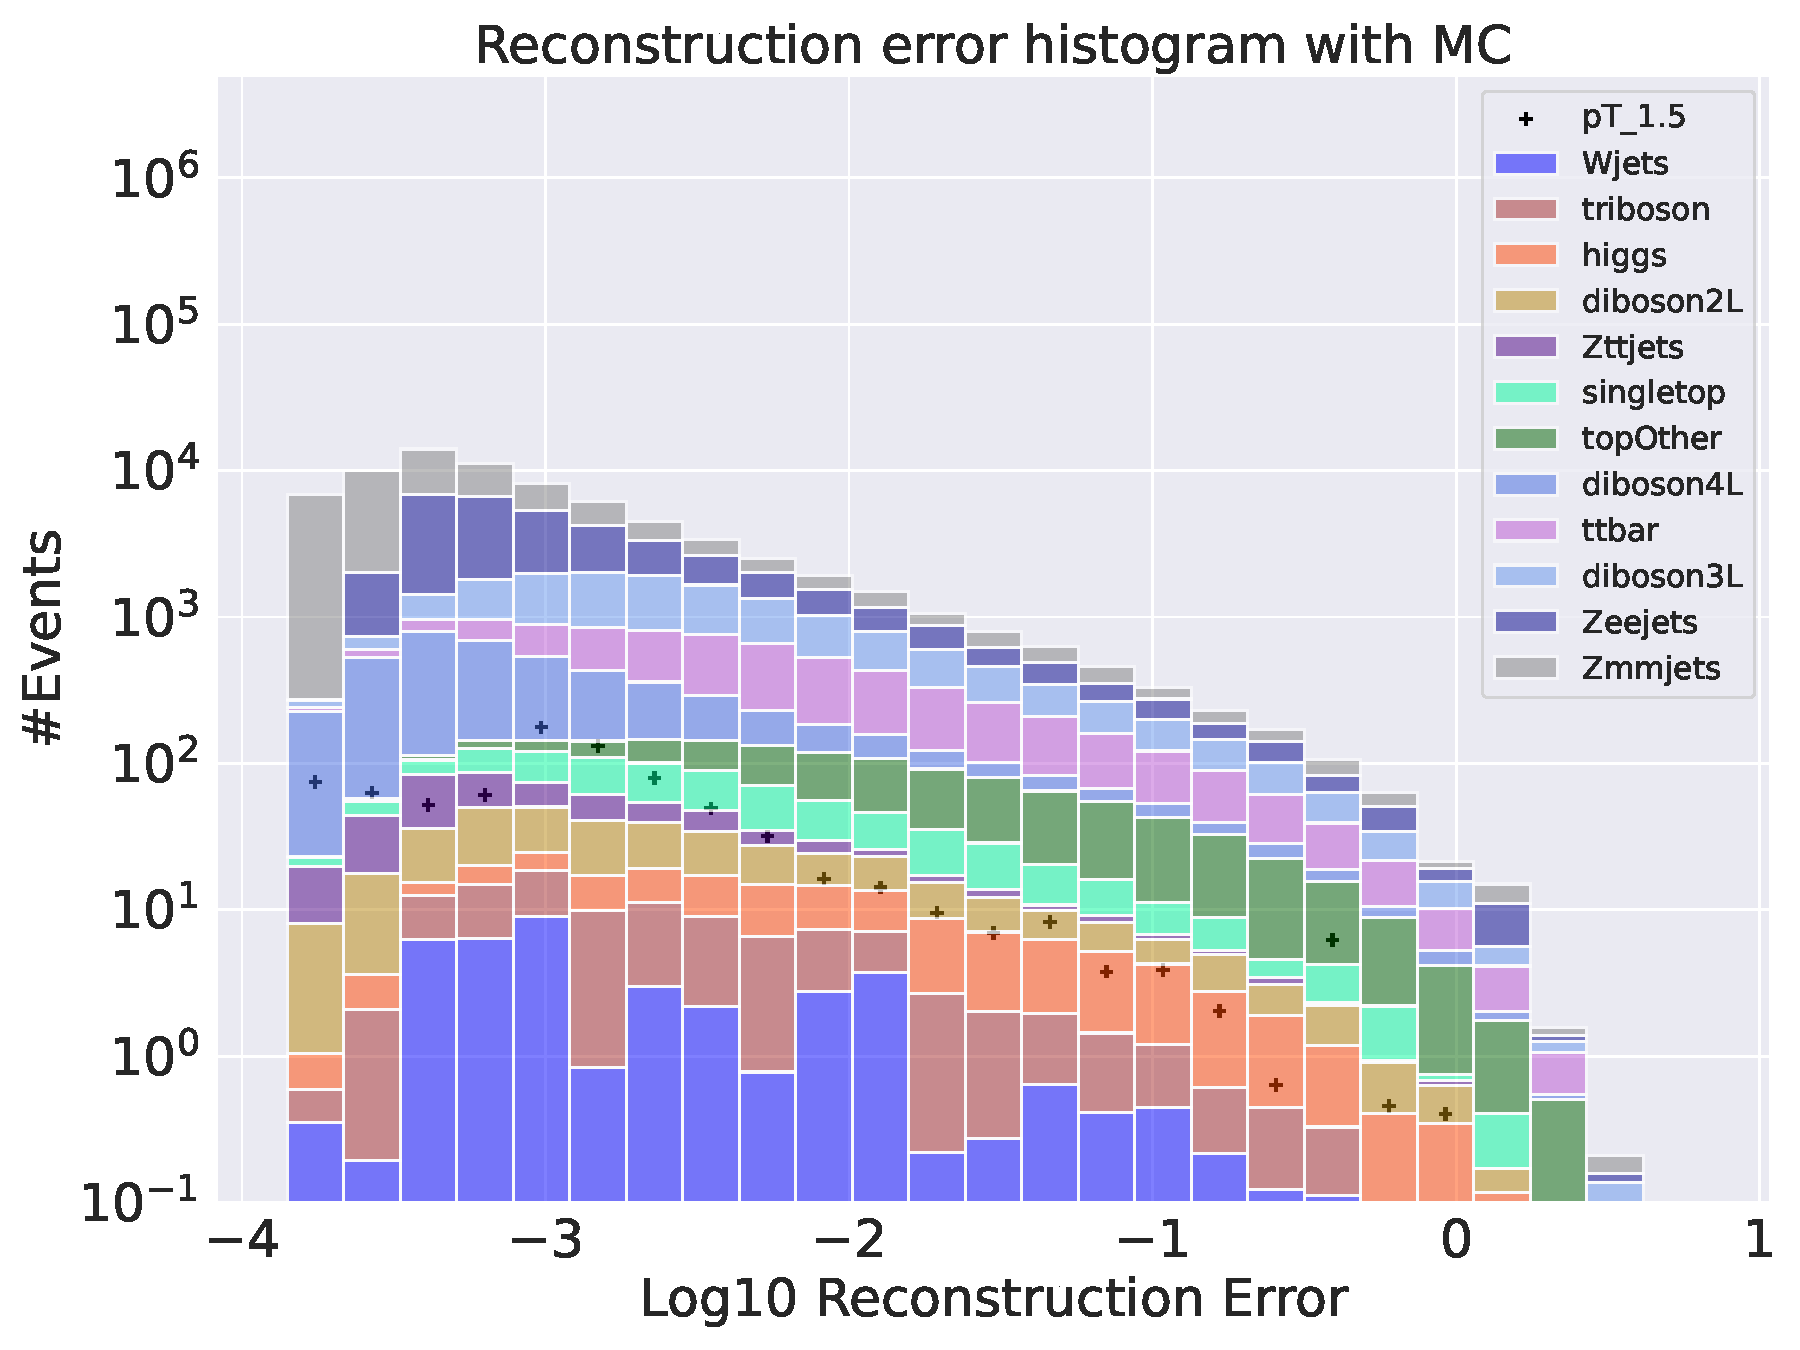
\includegraphics[width=\textwidth]{Figures/AE_testing/big/b_data_recon_big_rm3_feats_sig_pT_1.5.pdf}
        \caption{Reconstruction error on validation SM MC from the big variational Autoencoder.Here the signal is a subsample of the validation 
        set where the transverse momentum of the first electron and the first muon has been increased with a scale of $1.5$. The change of transverse 
        energy has thusly also been changed according to the scaling of transverse momentum. No significant difference in distributions are found. }
        \label{fig:ae_big_pt_1_5}
    \end{subfigure}
    \hfill 
    \caption{title}
    \label{fig:ae_big_small_pt_1_5}
\end{figure}

\begin{figure}[h!]
    \centering
    \begin{subfigure}{.45\textwidth}
        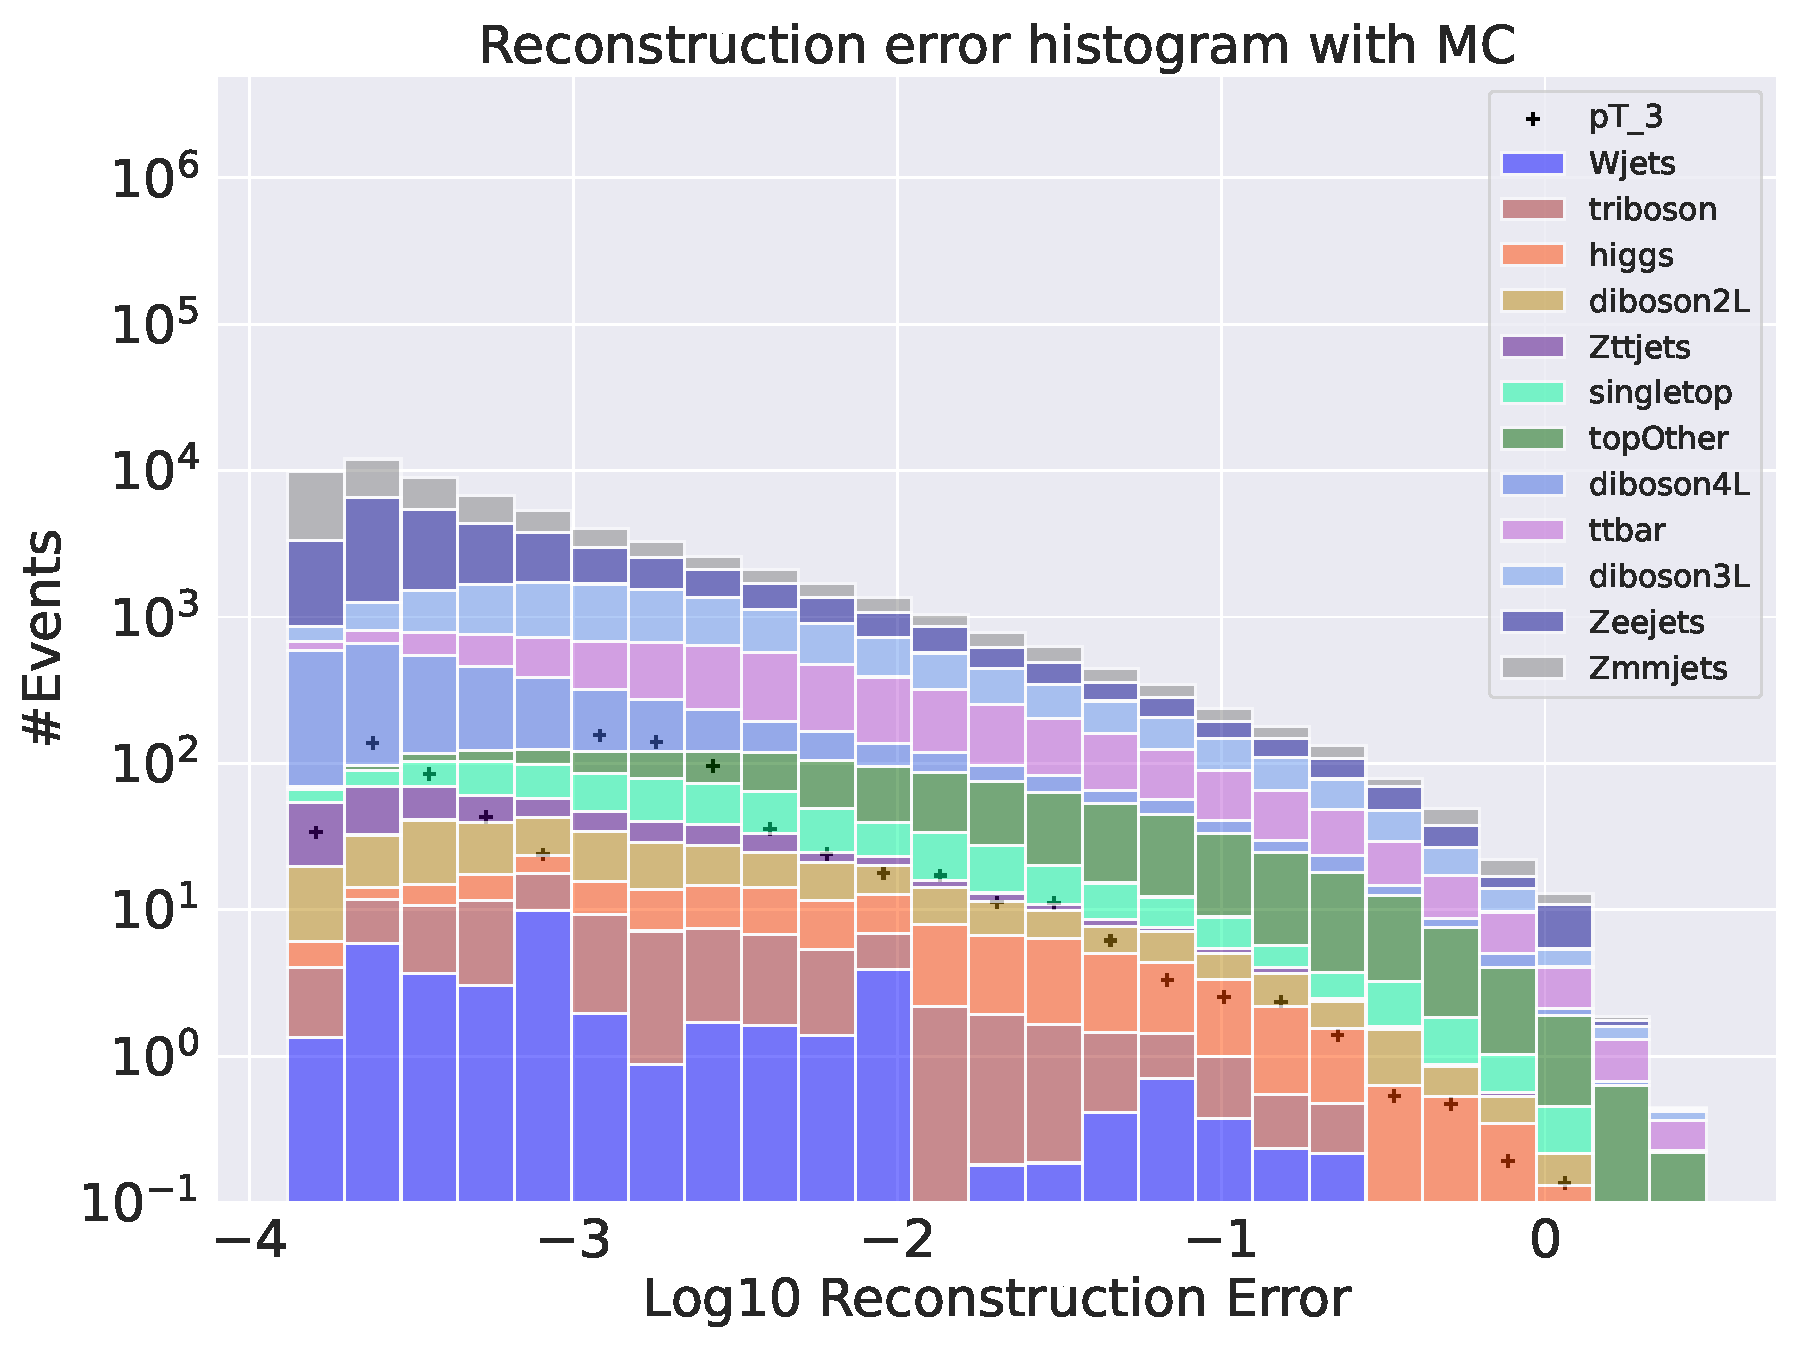
\includegraphics[width=\textwidth]{Figures/AE_testing/small/b_data_recon_big_rm3_feats_sig_pT_3.pdf}
        \caption{Reconstruction error on validation SM MC from the small variational Autoencoder. Here the signal is a subsample of the validation 
        set where the transverse momentum of the first electron and the first muon has been increased with a scale of $3$. The change of transverse 
        energy has thusly also been changed according to the scaling of transverse momentum. No significant difference in distributions are found. }
        \label{fig:ae_small_pt_3}
    \end{subfigure}
    \hfill 
    \begin{subfigure}{.45\textwidth}
        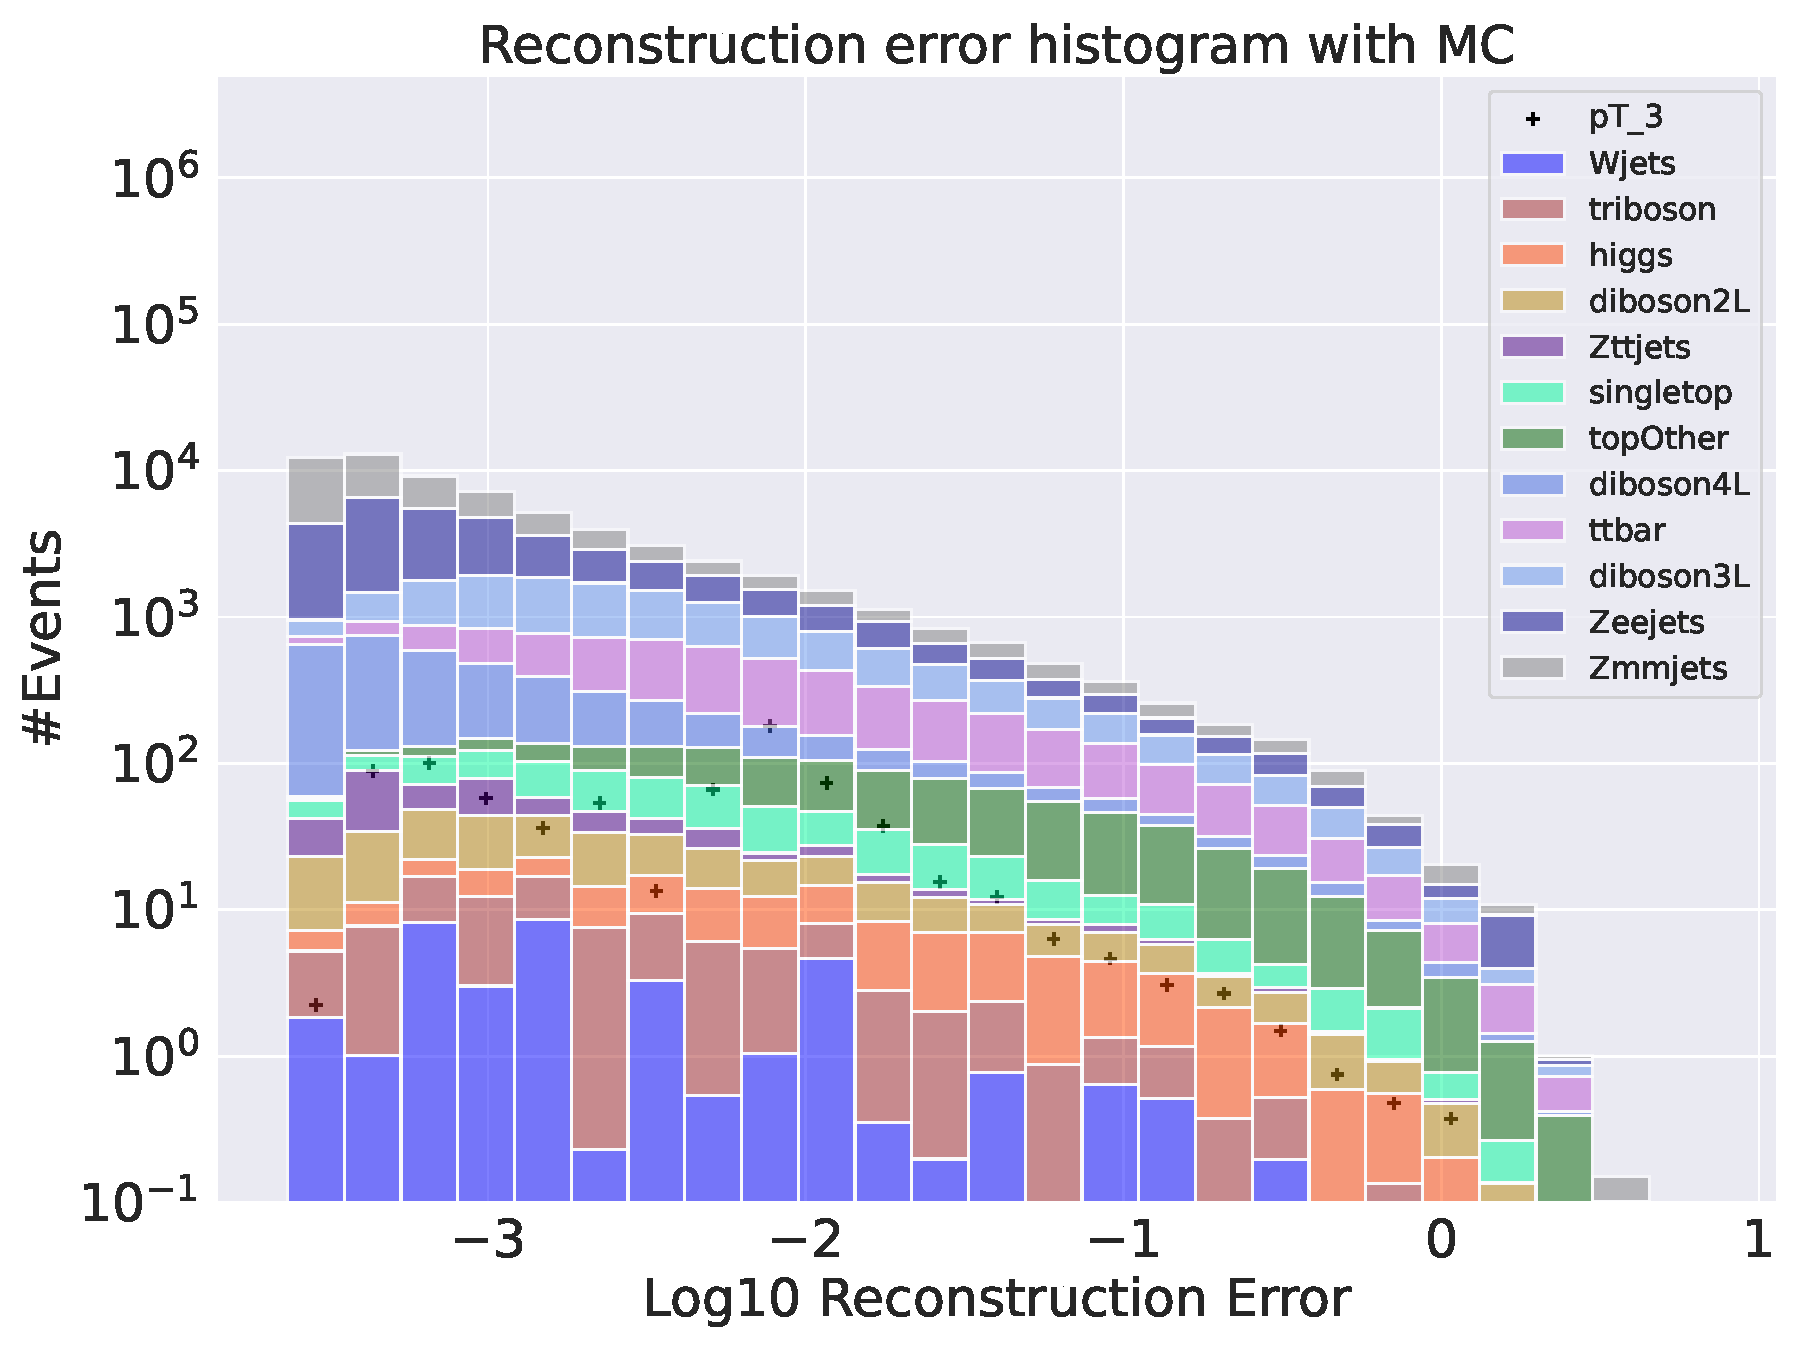
\includegraphics[width=\textwidth]{Figures/AE_testing/big/b_data_recon_big_rm3_feats_sig_pT_3.pdf}
        \caption{Reconstruction error on validation SM MC from the big variational Autoencoder. Here the signal is a subsample of the validation 
        set where the transverse momentum of the first electron and the first muon has been increased with a scale of $3$. The change of transverse 
        energy has thusly also been changed according to the scaling of transverse momentum. No significant difference in distributions are found. }
        \label{fig:ae_big_pt_3}
    \end{subfigure}
    \hfill 
    \caption{title}
    \label{fig:ae_big_small_pt_3}
\end{figure}

\begin{figure}[h!]
    \centering
    \begin{subfigure}{.45\textwidth}
        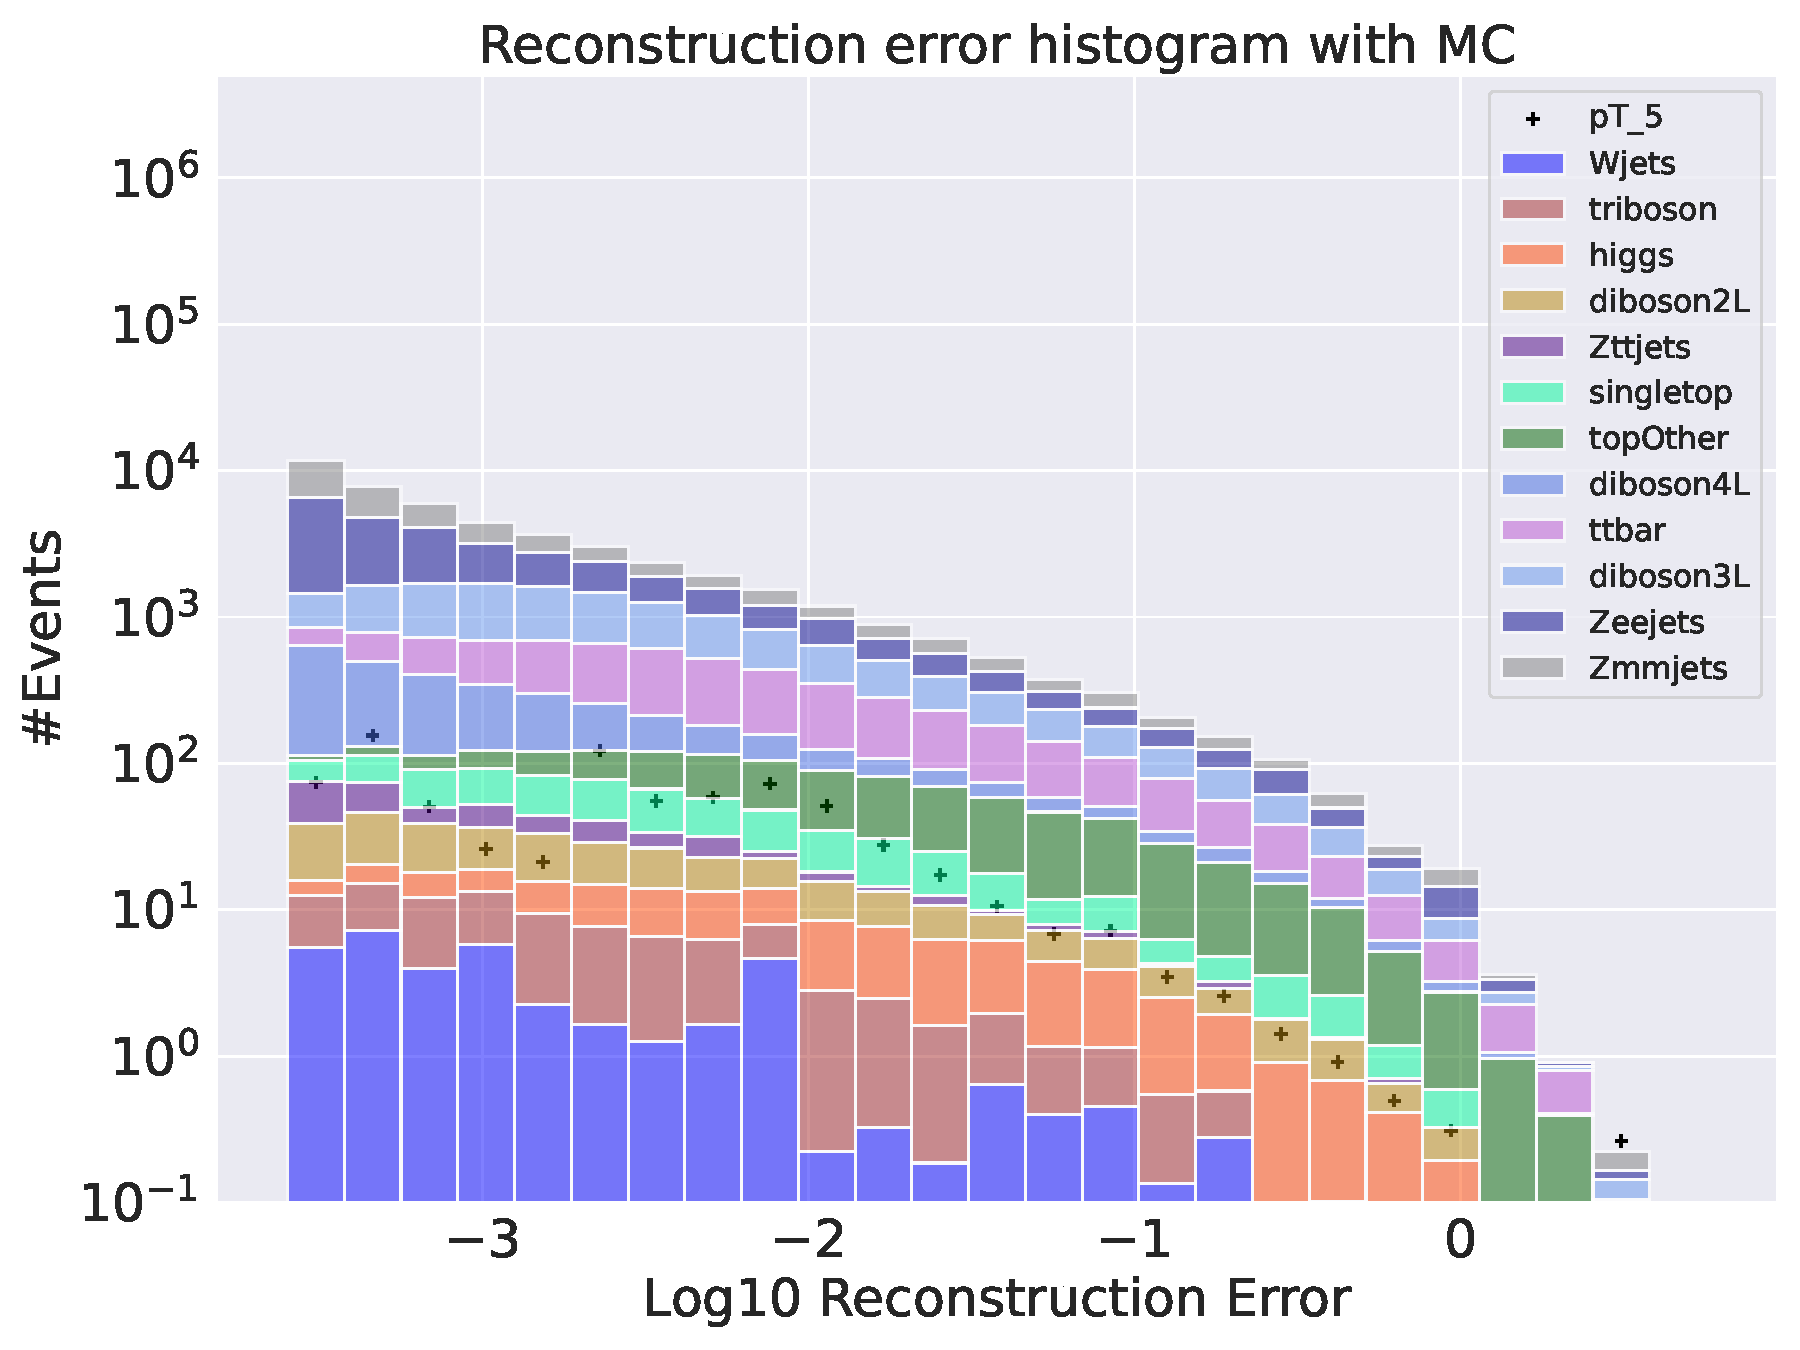
\includegraphics[width=\textwidth]{Figures/AE_testing/small/b_data_recon_big_rm3_feats_sig_pT_5.pdf}
        \caption{Reconstruction error on validation SM MC from the small variational Autoencoder. Here the signal is a subsample of the validation 
        set where the transverse momentum of the first electron and the first muon has been increased with a scale of $5$. The change of transverse 
        energy has thusly also been changed according to the scaling of transverse momentum. No significant difference in distributions are found. }
        \label{fig:ae_small_pt_5}
    \end{subfigure}
    \hfill 
    \begin{subfigure}{.45\textwidth}
        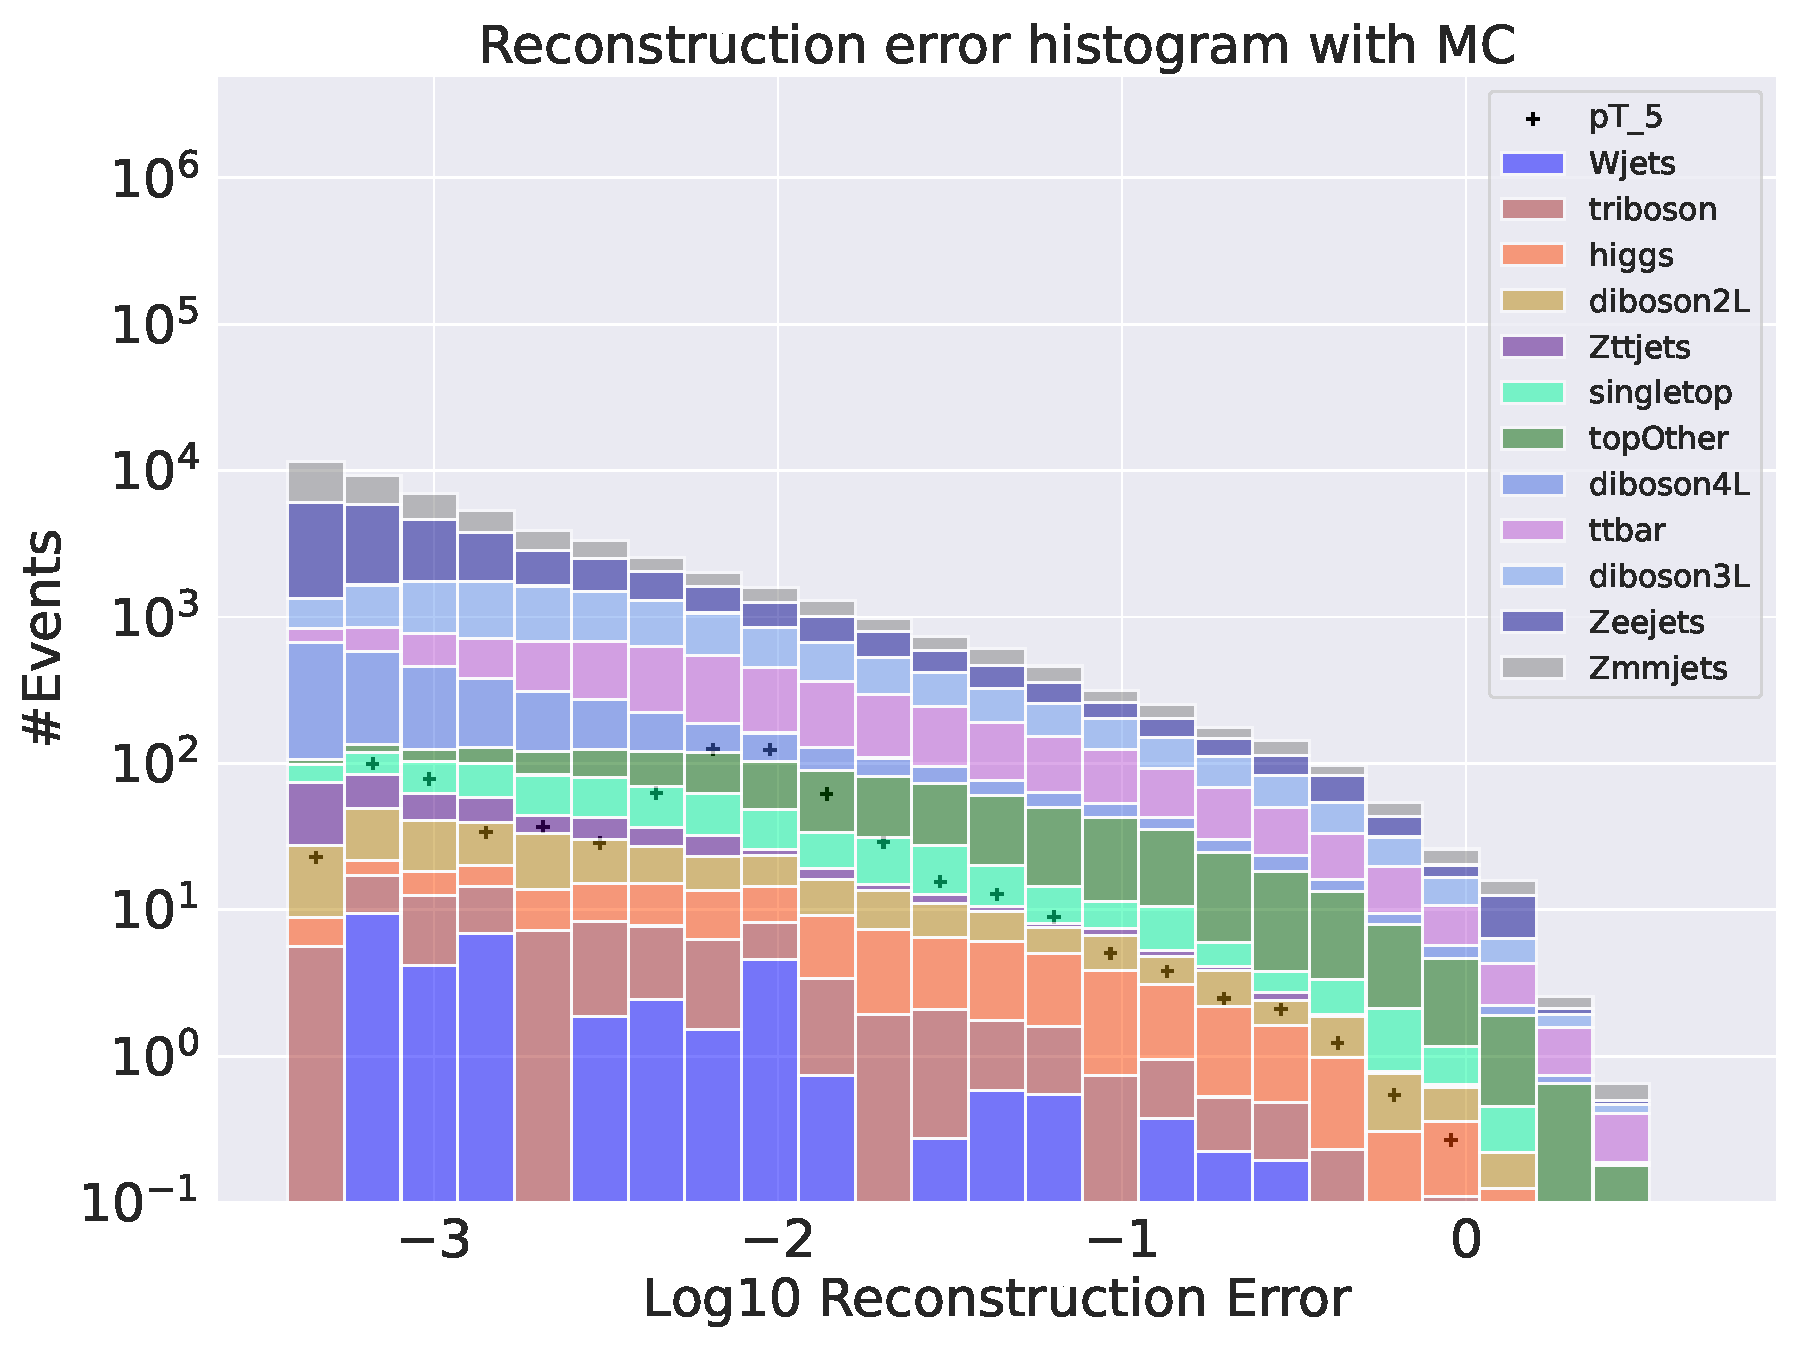
\includegraphics[width=\textwidth]{Figures/AE_testing/big/b_data_recon_big_rm3_feats_sig_pT_5.pdf}
        \caption{Reconstruction error on validation SM MC from the big variational Autoencoder. Here the signal is a subsample of the validation 
        set where the transverse momentum of the first electron and the first muon has been increased with a scale of $5$. The change of transverse 
        energy has thusly also been changed according to the scaling of transverse momentum. No significant difference in distributions are found. }
        \label{fig:ae_big_pt_5}
    \end{subfigure}
    \hfill 
    \caption{title}
    \label{fig:ae_big_small_pt_5}
\end{figure}


\begin{figure}[h!]
    \centering
    \begin{subfigure}{.45\textwidth}
        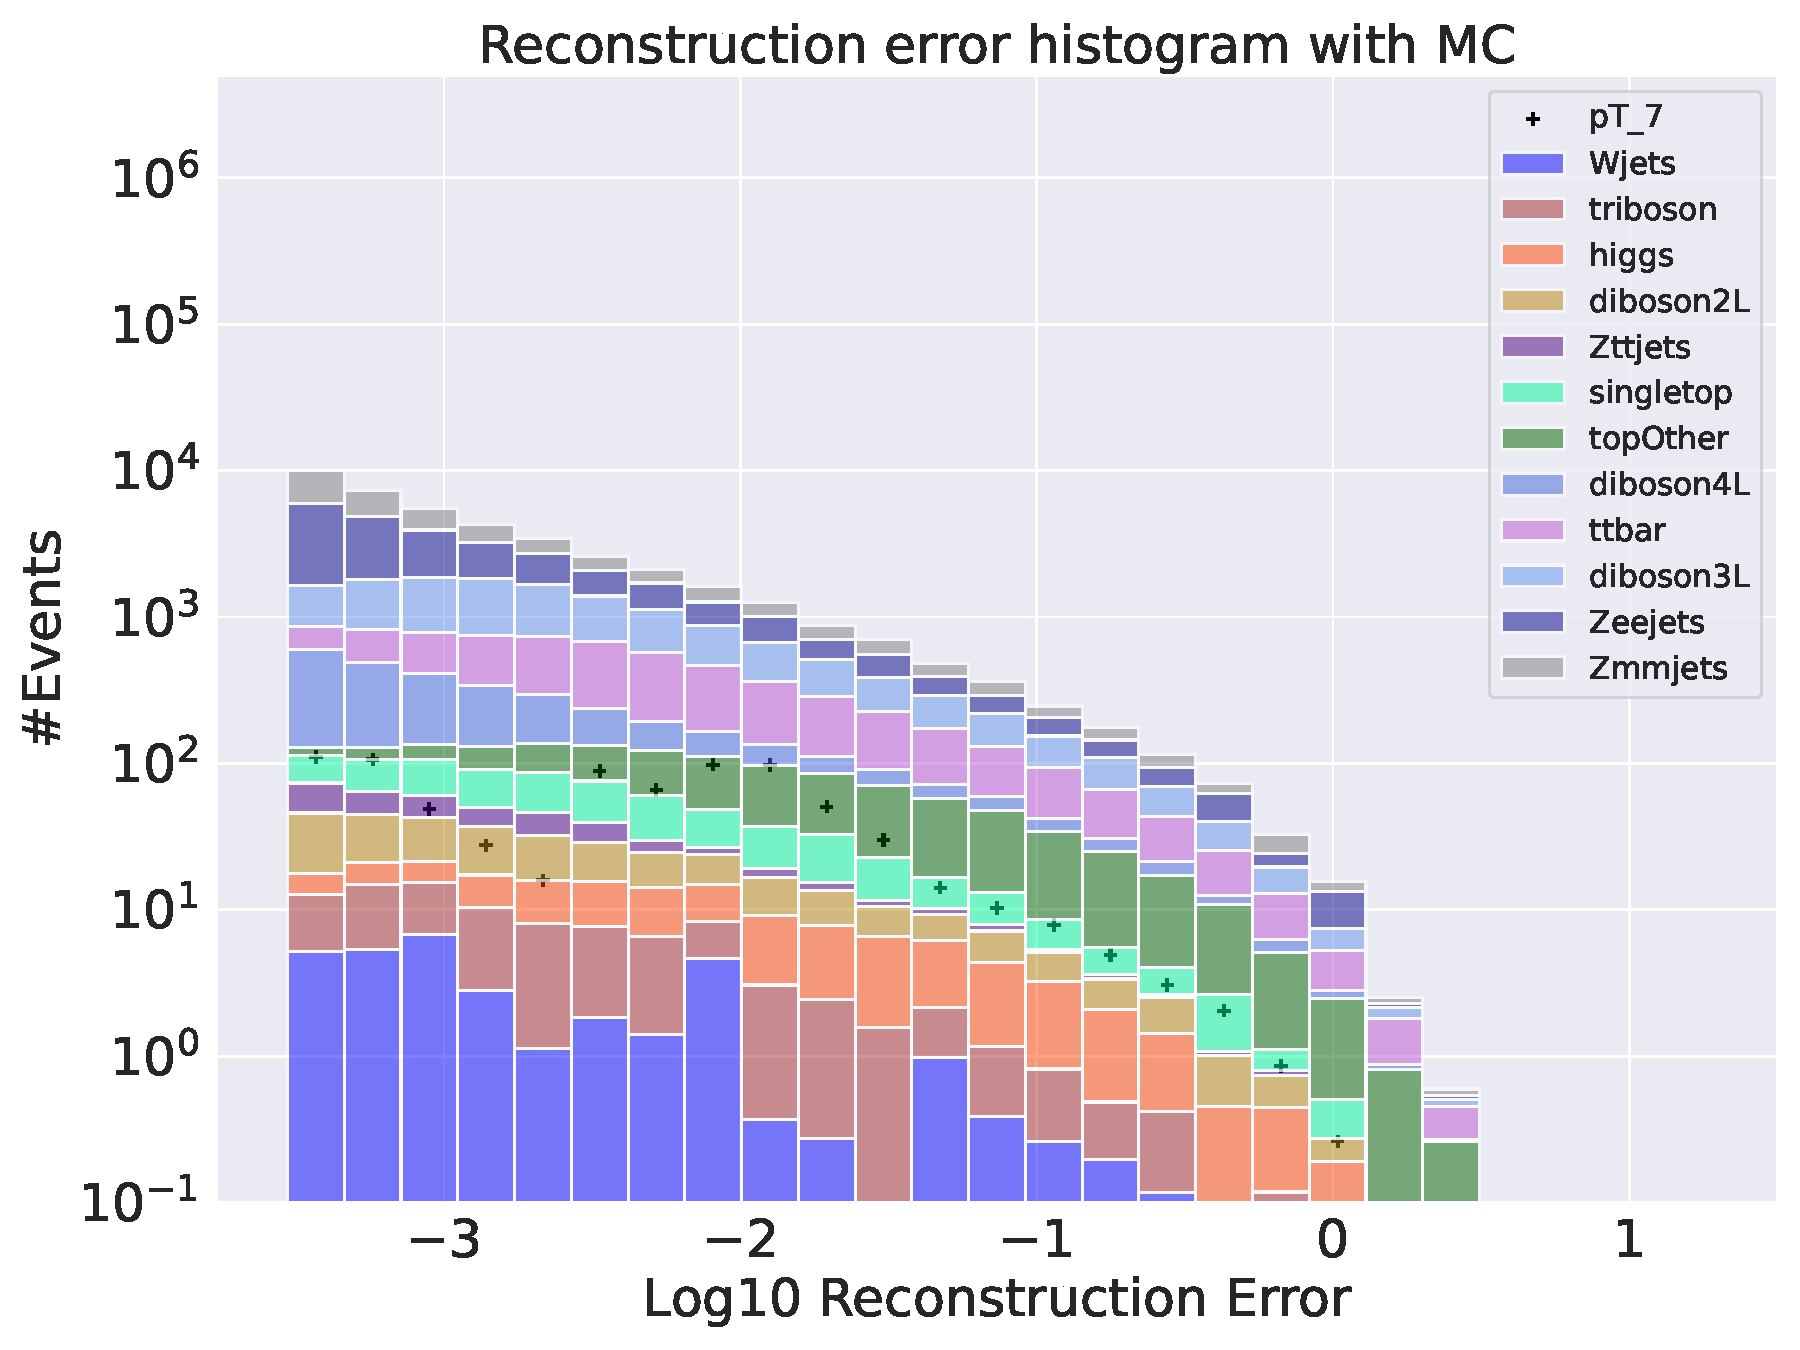
\includegraphics[width=\textwidth]{Figures/AE_testing/small/b_data_recon_big_rm3_feats_sig_pT_7.pdf}
        \caption{Reconstruction error on validation SM MC from the small variational Autoencoder. Here the signal is a subsample of the validation 
        set where the transverse momentum of the first electron and the first muon has been increased with a scale of $7$. The change of transverse 
        energy has thusly also been changed according to the scaling of transverse momentum. No significant difference in distributions are found. }
        \label{fig:ae_small_pt_7}
    \end{subfigure}
    \hfill 
    \begin{subfigure}{.45\textwidth}
        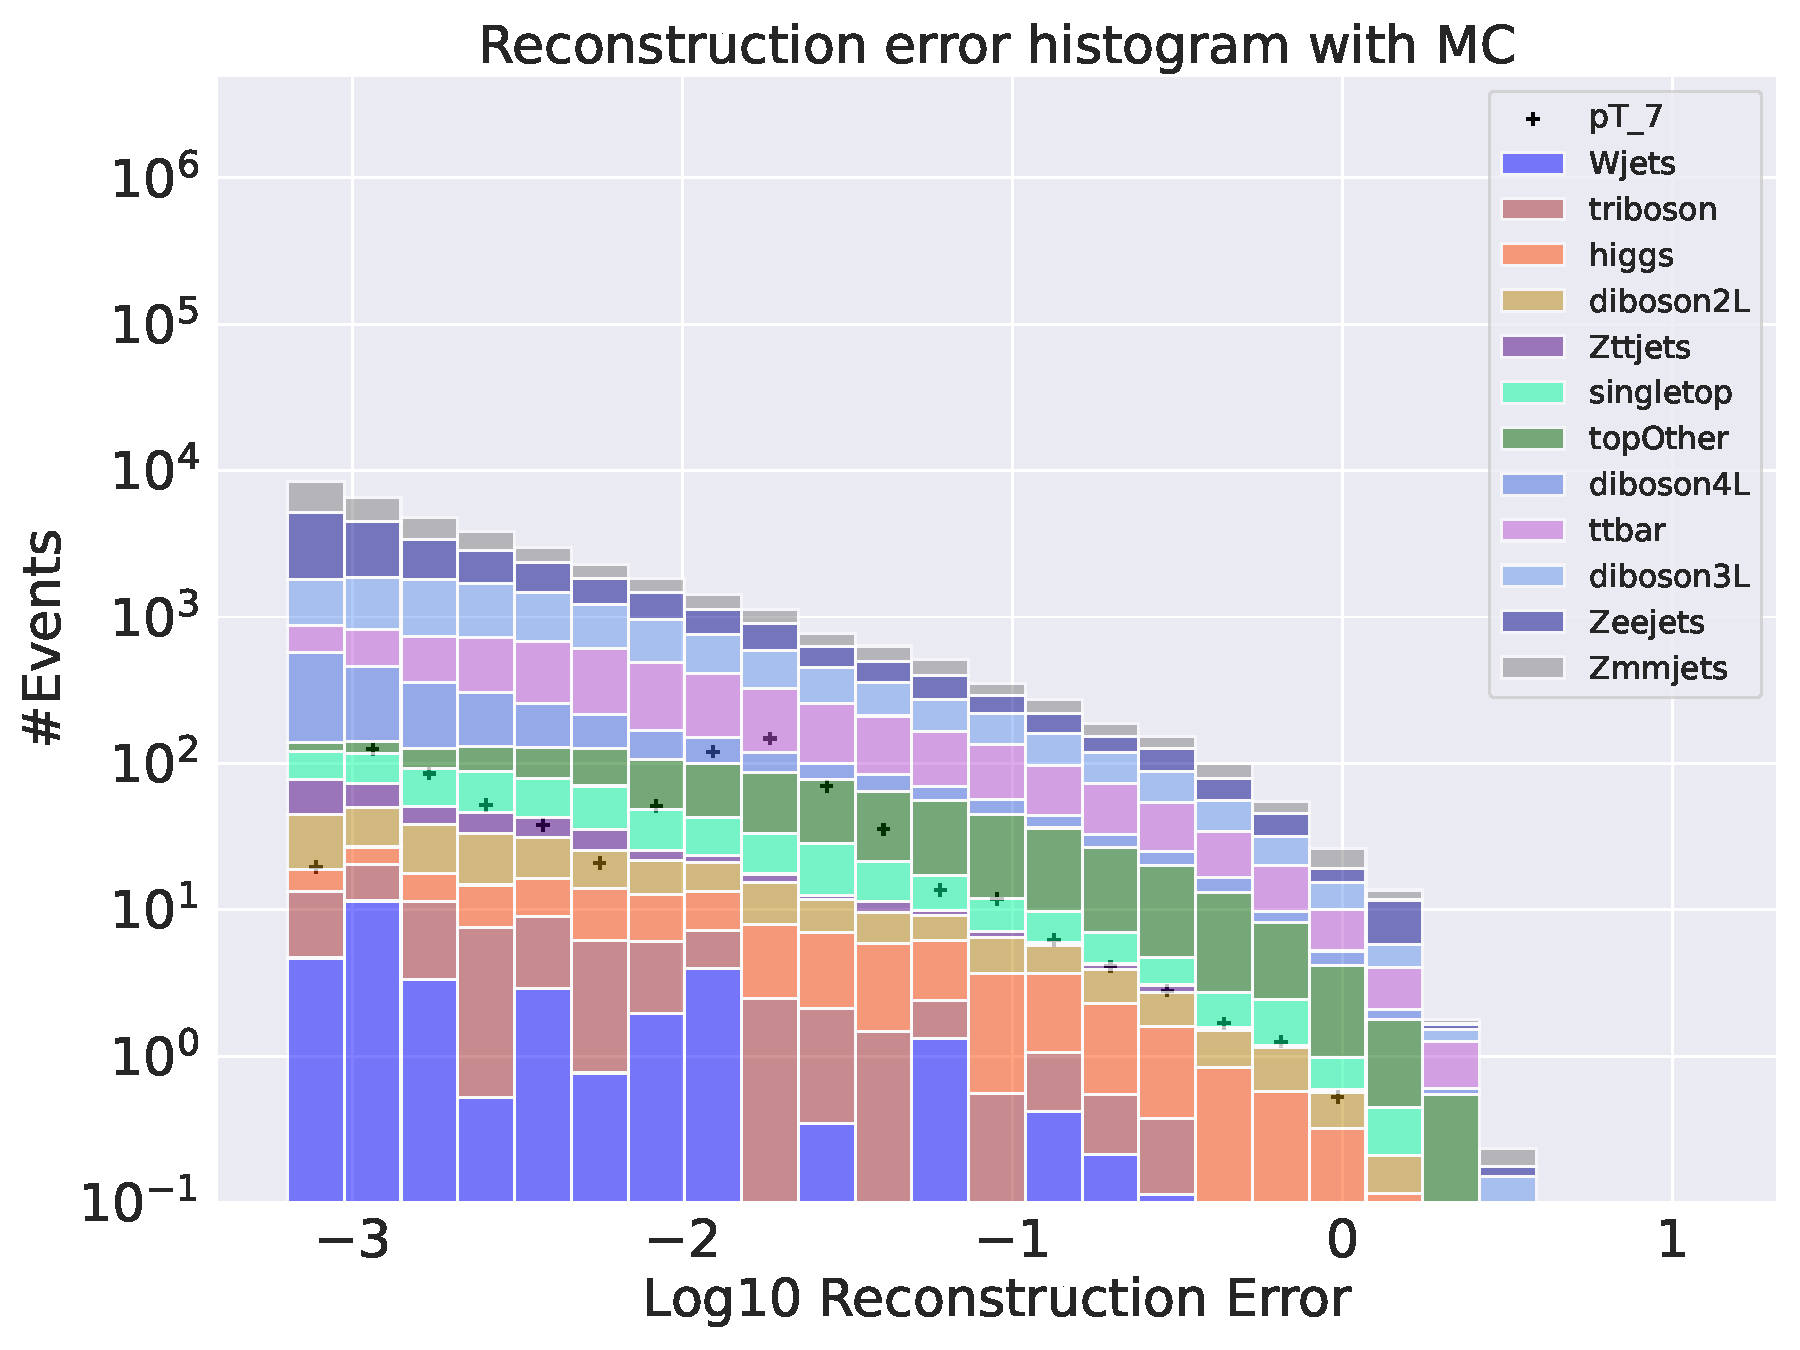
\includegraphics[width=\textwidth]{Figures/AE_testing/big/b_data_recon_big_rm3_feats_sig_pT_7.pdf}
        \caption{Reconstruction error on validation SM MC from the big variational Autoencoder. Here the signal is a subsample of the validation 
        set where the transverse momentum of the first electron and the first muon has been increased with a scale of $7$. The change of transverse 
        energy has thusly also been changed according to the scaling of transverse momentum. No significant difference in distributions are found. }
        \label{fig:ae_big_pt_7}
    \end{subfigure}
    \hfill 
    \caption{title}
    \label{fig:ae_big_small_pt_7}
\end{figure}

\begin{figure}[h!]
    \centering
    \begin{subfigure}{.45\textwidth}
        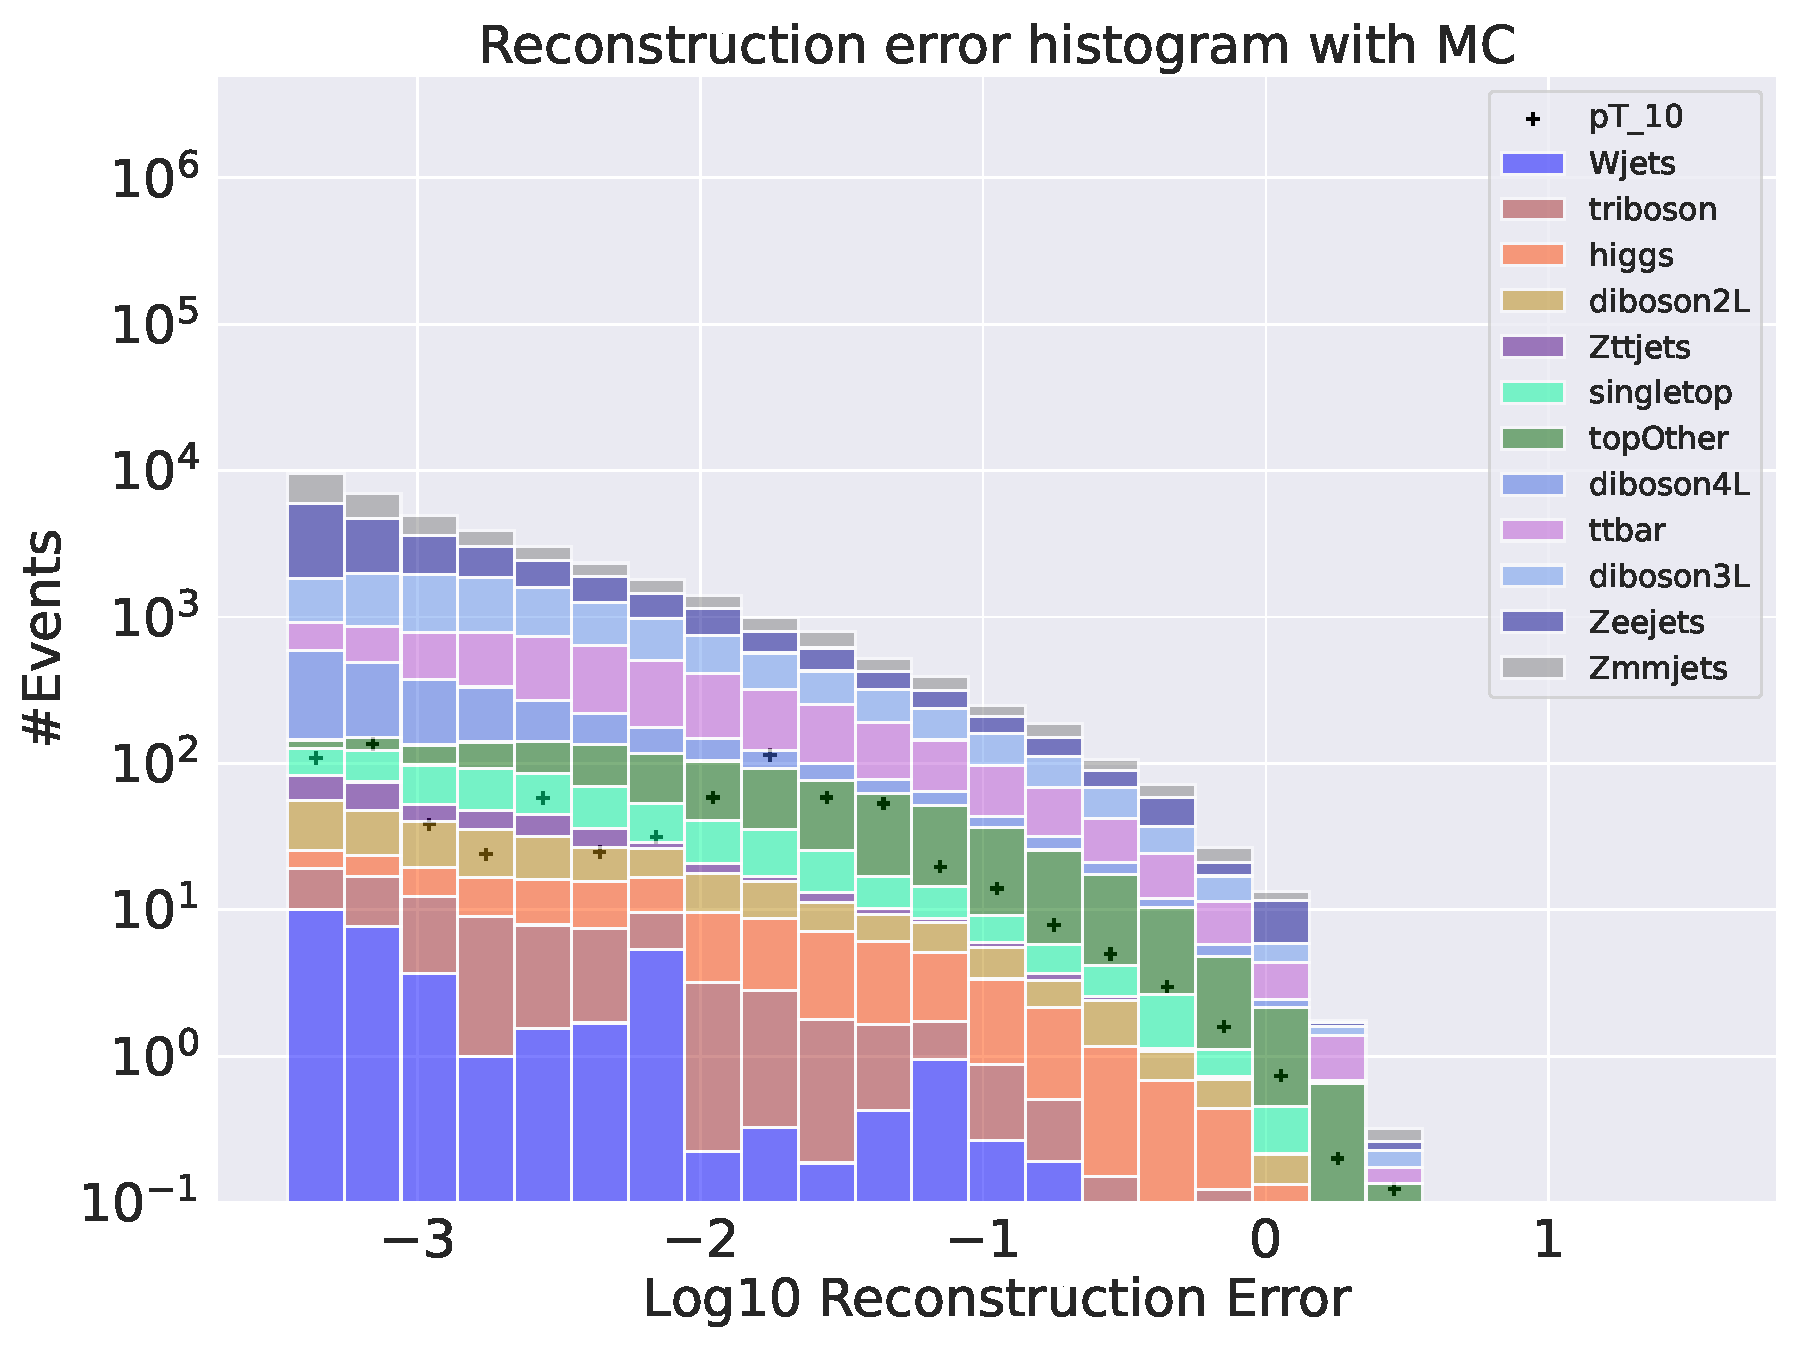
\includegraphics[width=\textwidth]{Figures/AE_testing/small/b_data_recon_big_rm3_feats_sig_pT_10.pdf}
        \caption{Reconstruction error on validation SM MC from the small variational Autoencoder. Here the signal is a subsample of the validation 
        set where the transverse momentum of the first electron and the first muon has been increased with a scale of $10$. The change of transverse 
        energy has thusly also been changed according to the scaling of transverse momentum. No significant difference in distributions are found. }
        \label{fig:ae_small_pt_10}
    \end{subfigure}
    \hfill 
    \begin{subfigure}{.45\textwidth}
        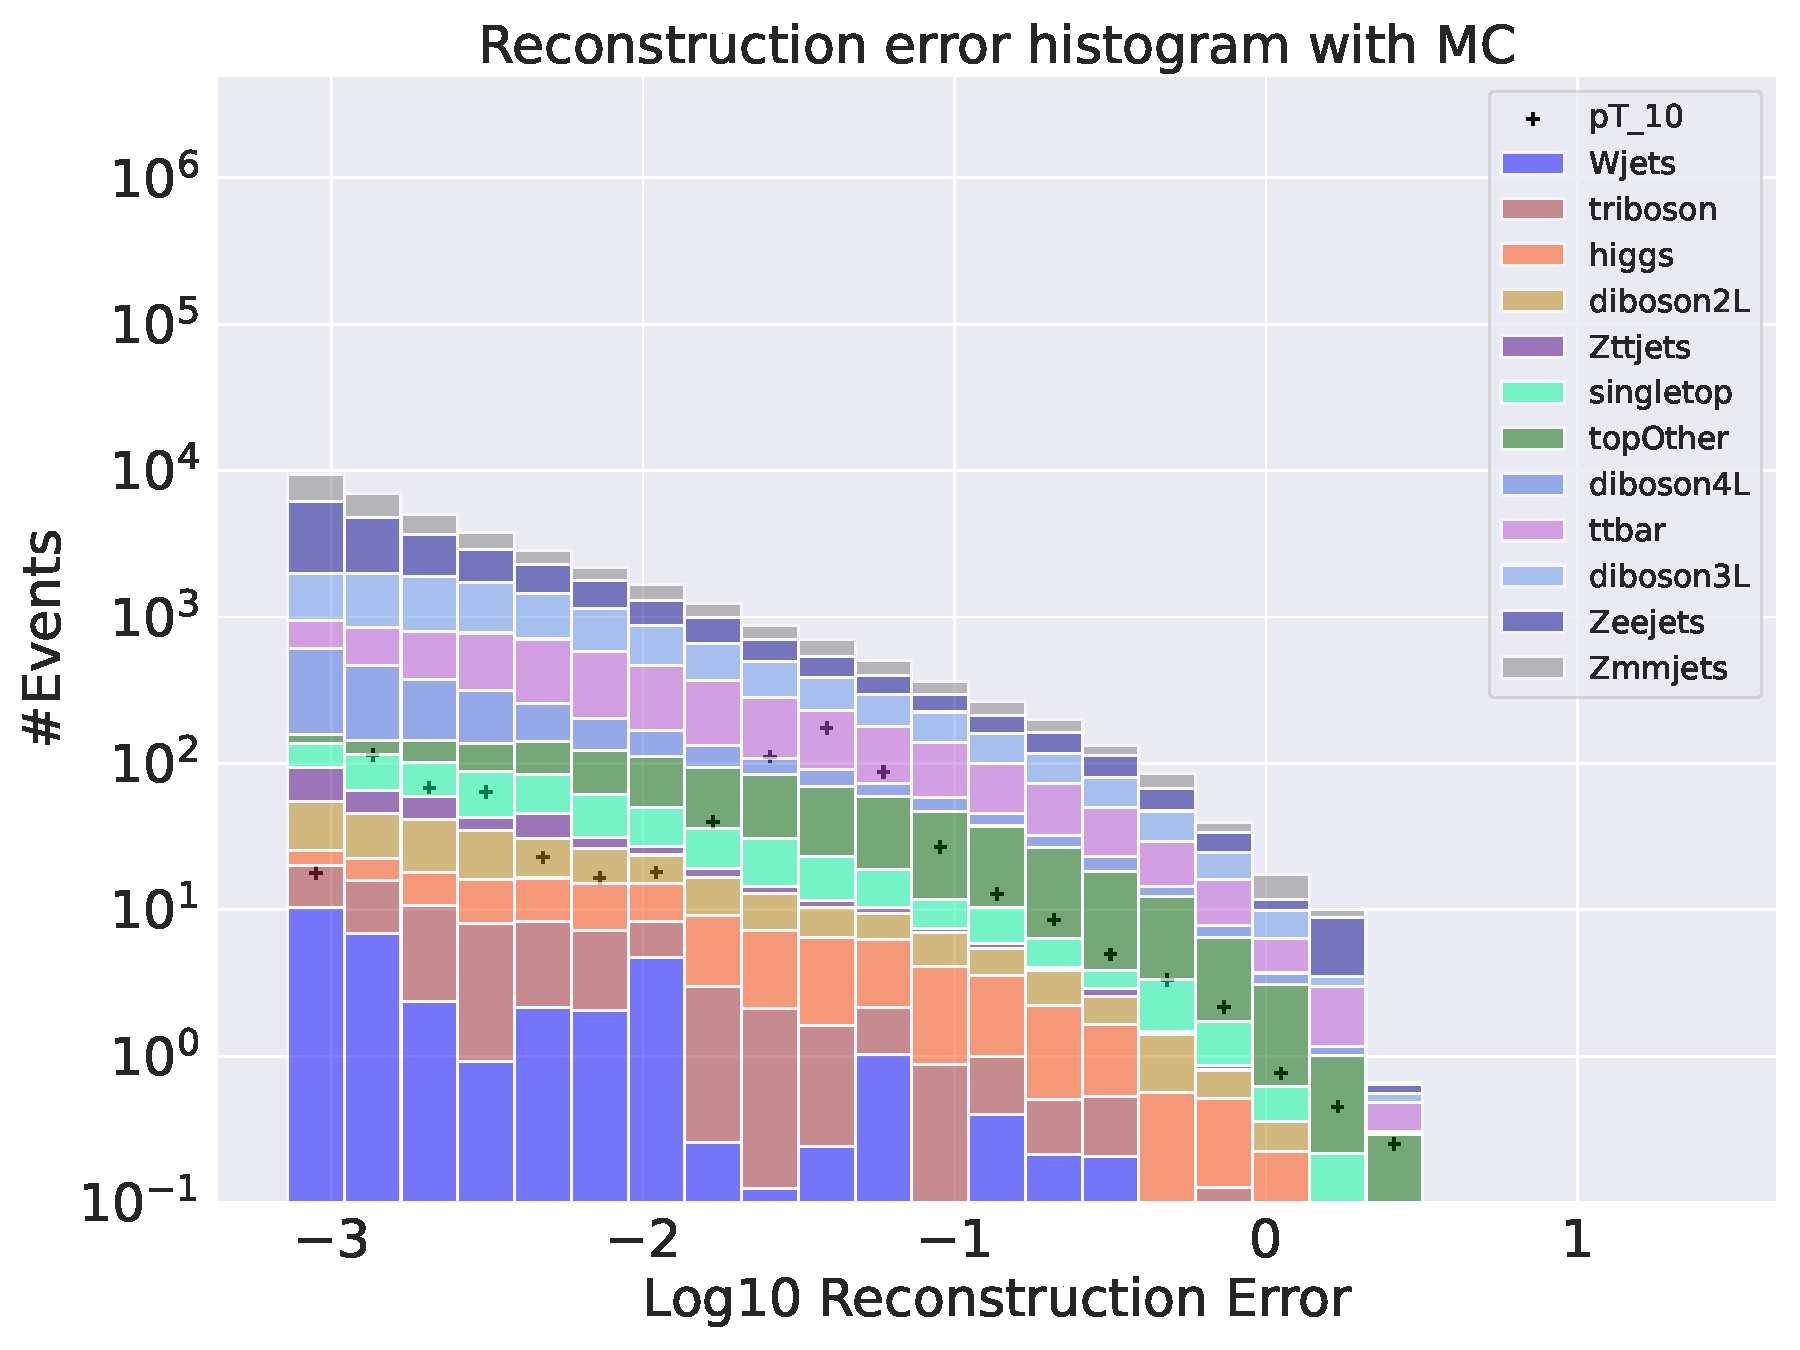
\includegraphics[width=\textwidth]{Figures/AE_testing/big/b_data_recon_big_rm3_feats_sig_pT_10.pdf}
        \caption{Reconstruction error on validation SM MC from the big variational Autoencoder. Here the signal is a subsample of the validation 
        set where the transverse momentum of the first electron and the first muon has been increased with a scale of $10$. The change of transverse 
        energy has thusly also been changed according to the scaling of transverse momentum. No significant difference in distributions are found. }
        \label{fig:ae_big_pt_10}
    \end{subfigure}
    \hfill 
    \caption{title}
    \label{fig:ae_big_small_pt_10}
\end{figure}



\subsubsection*{Variational Autoencoder}

\begin{figure}[h!]
    \centering
    \begin{subfigure}{.45\textwidth}
        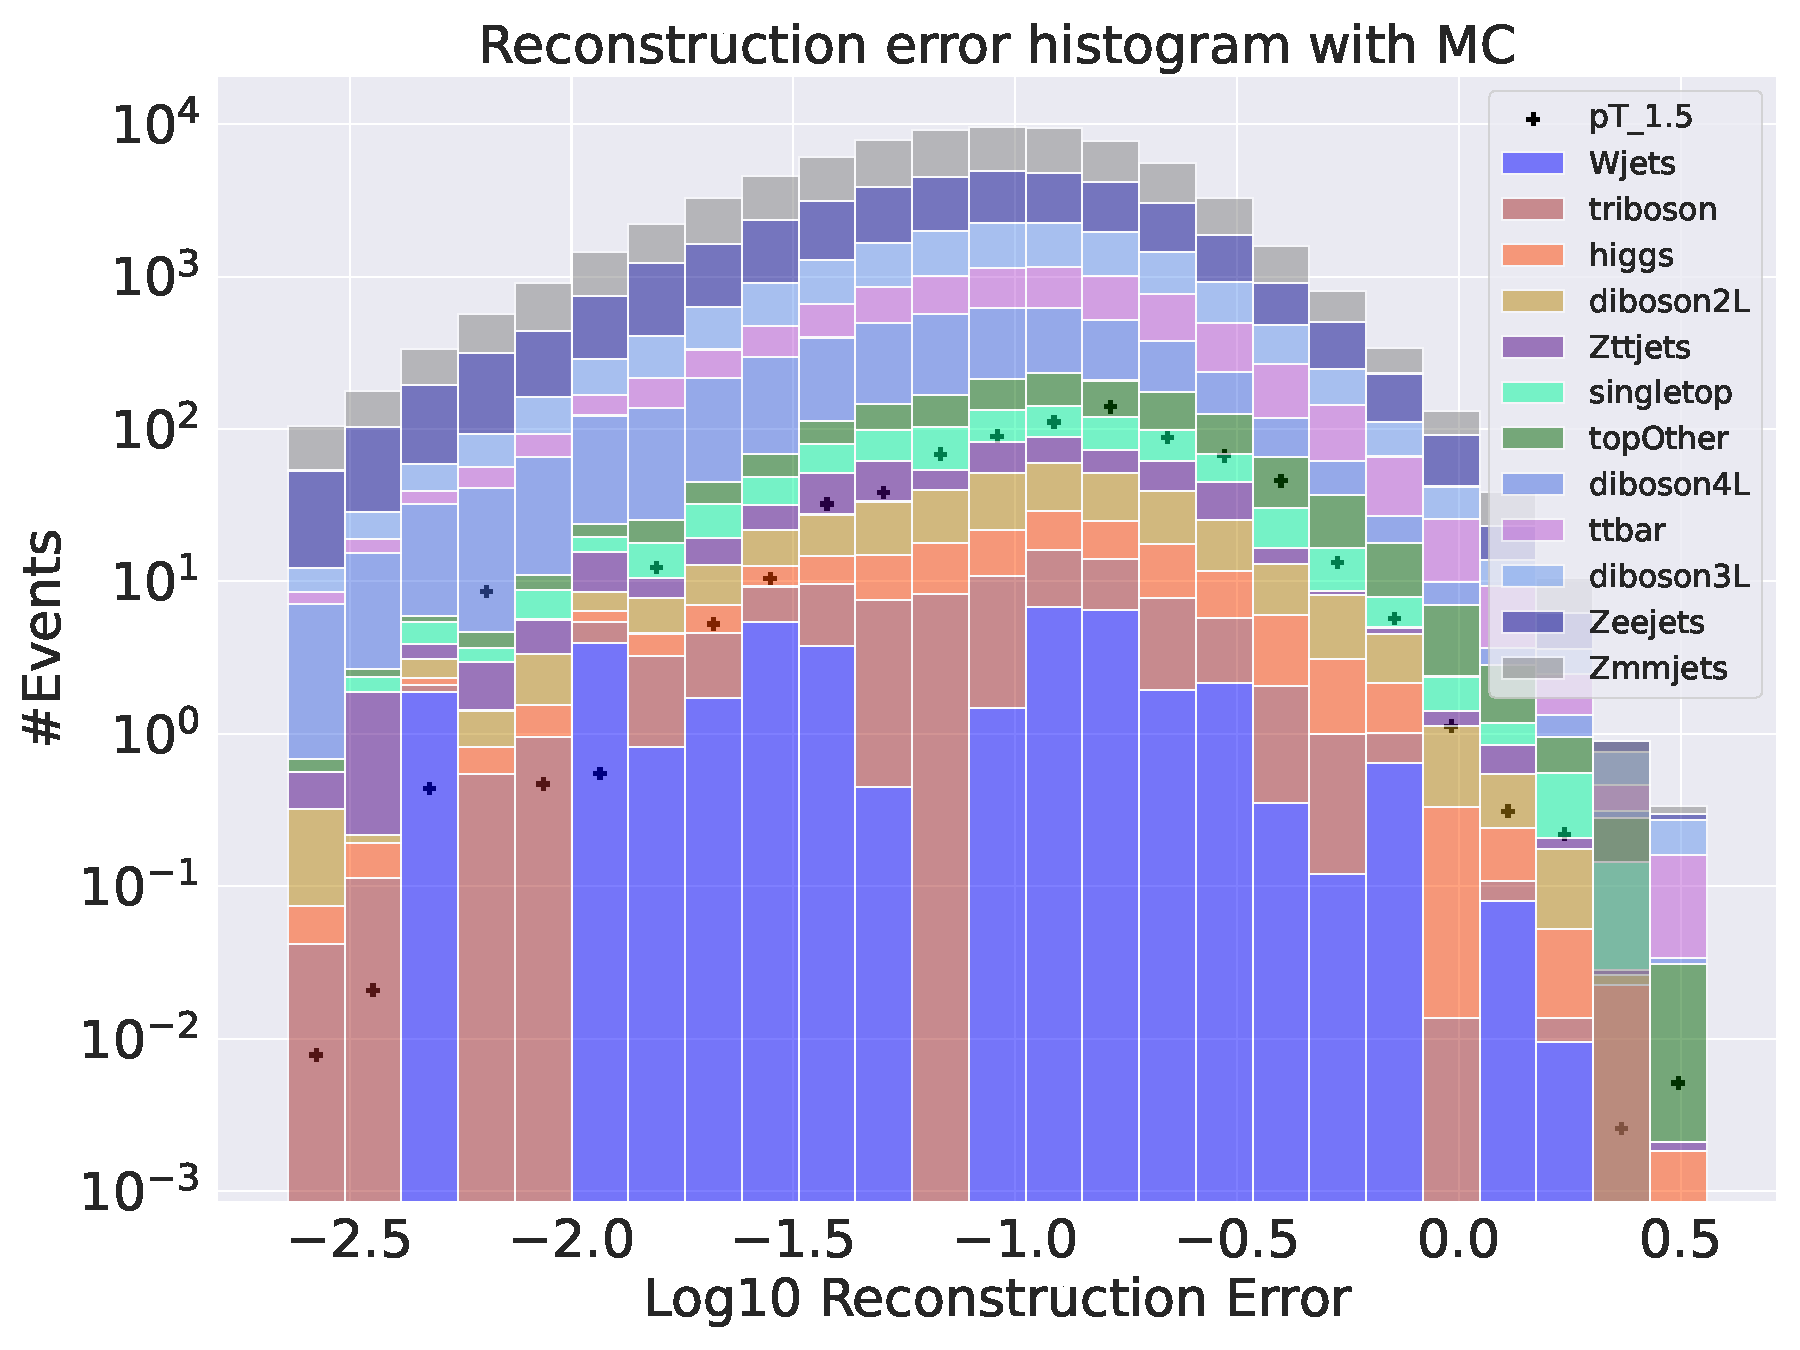
\includegraphics[width=\textwidth]{Figures/VAE_testing/small/b_data_recon_big_rm3_feats_sig_pT_1.5.pdf}
        \caption{Reconstruction error on validation SM MC from the small variational Autoencoder. Here the signal is a subsample of the validation 
        set where the transverse momentum of the first electron and the first muon has been increased with a scale of $1.5$. The change of transverse 
        energy has thusly also been changed according to the scaling of transverse momentum. No significant difference in distributions are found. }
        \label{fig:VAE_small_pt_1_5}
    \end{subfigure}
    \hfill 
    \begin{subfigure}{.45\textwidth}
        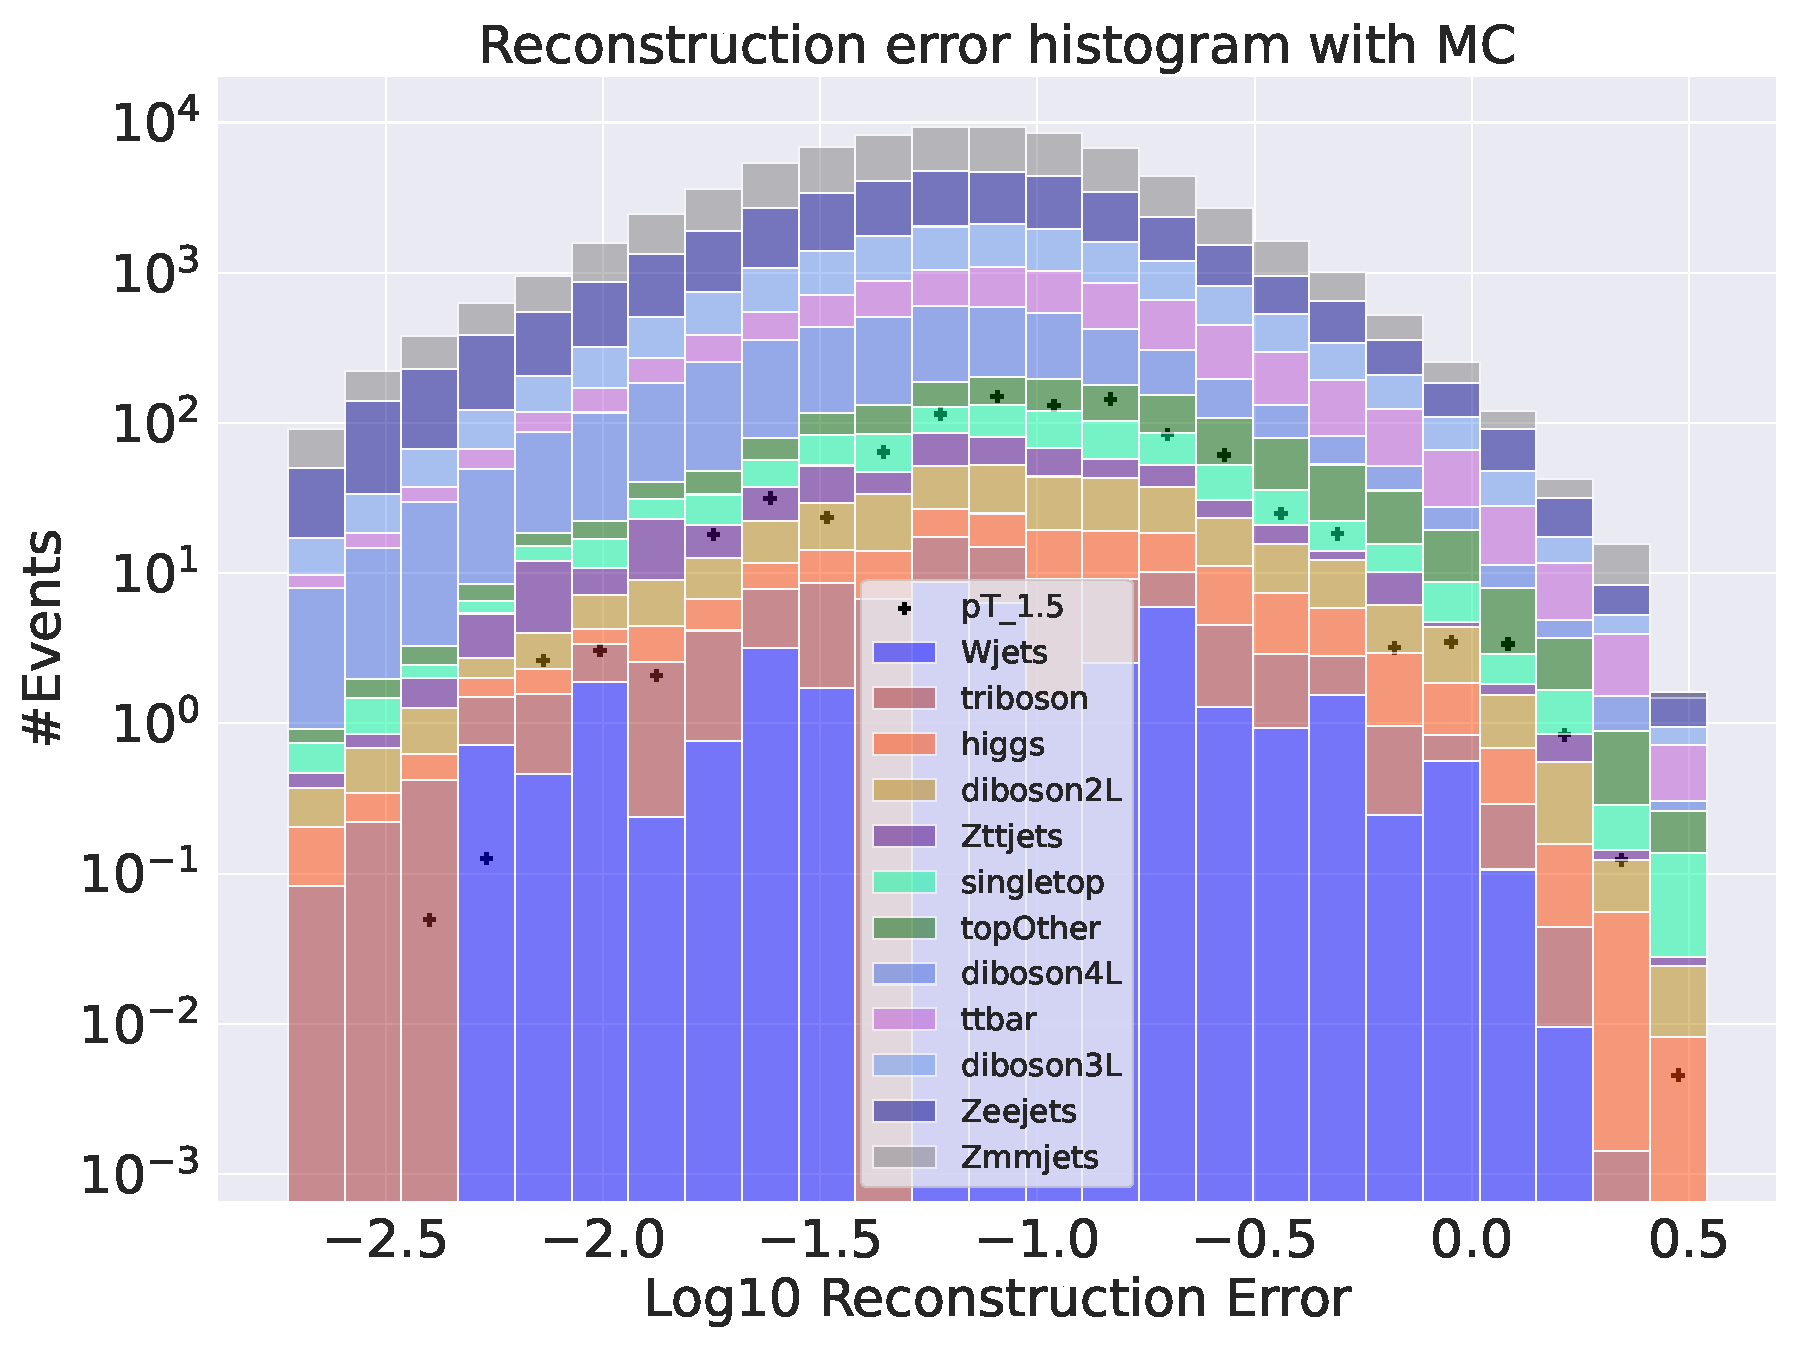
\includegraphics[width=\textwidth]{Figures/VAE_testing/big/b_data_recon_big_rm3_feats_sig_pT_1.5.pdf}
        \caption{Reconstruction error on validation SM MC from the big variational Autoencoder. Here the signal is a subsample of the validation 
        set where the transverse momentum of the first electron and the first muon has been increased with a scale of $1.5$. The change of transverse 
        energy has thusly also been changed according to the scaling of transverse momentum. No significant difference in distributions are found. }
        \label{fig:VAE_big_pt_1_5}
    \end{subfigure}
    \hfill 
    \caption{title}
    \label{fig:VAE_big_small_pt_1_5}
\end{figure}

\begin{figure}[h!]
    \centering
    \begin{subfigure}{.45\textwidth}
        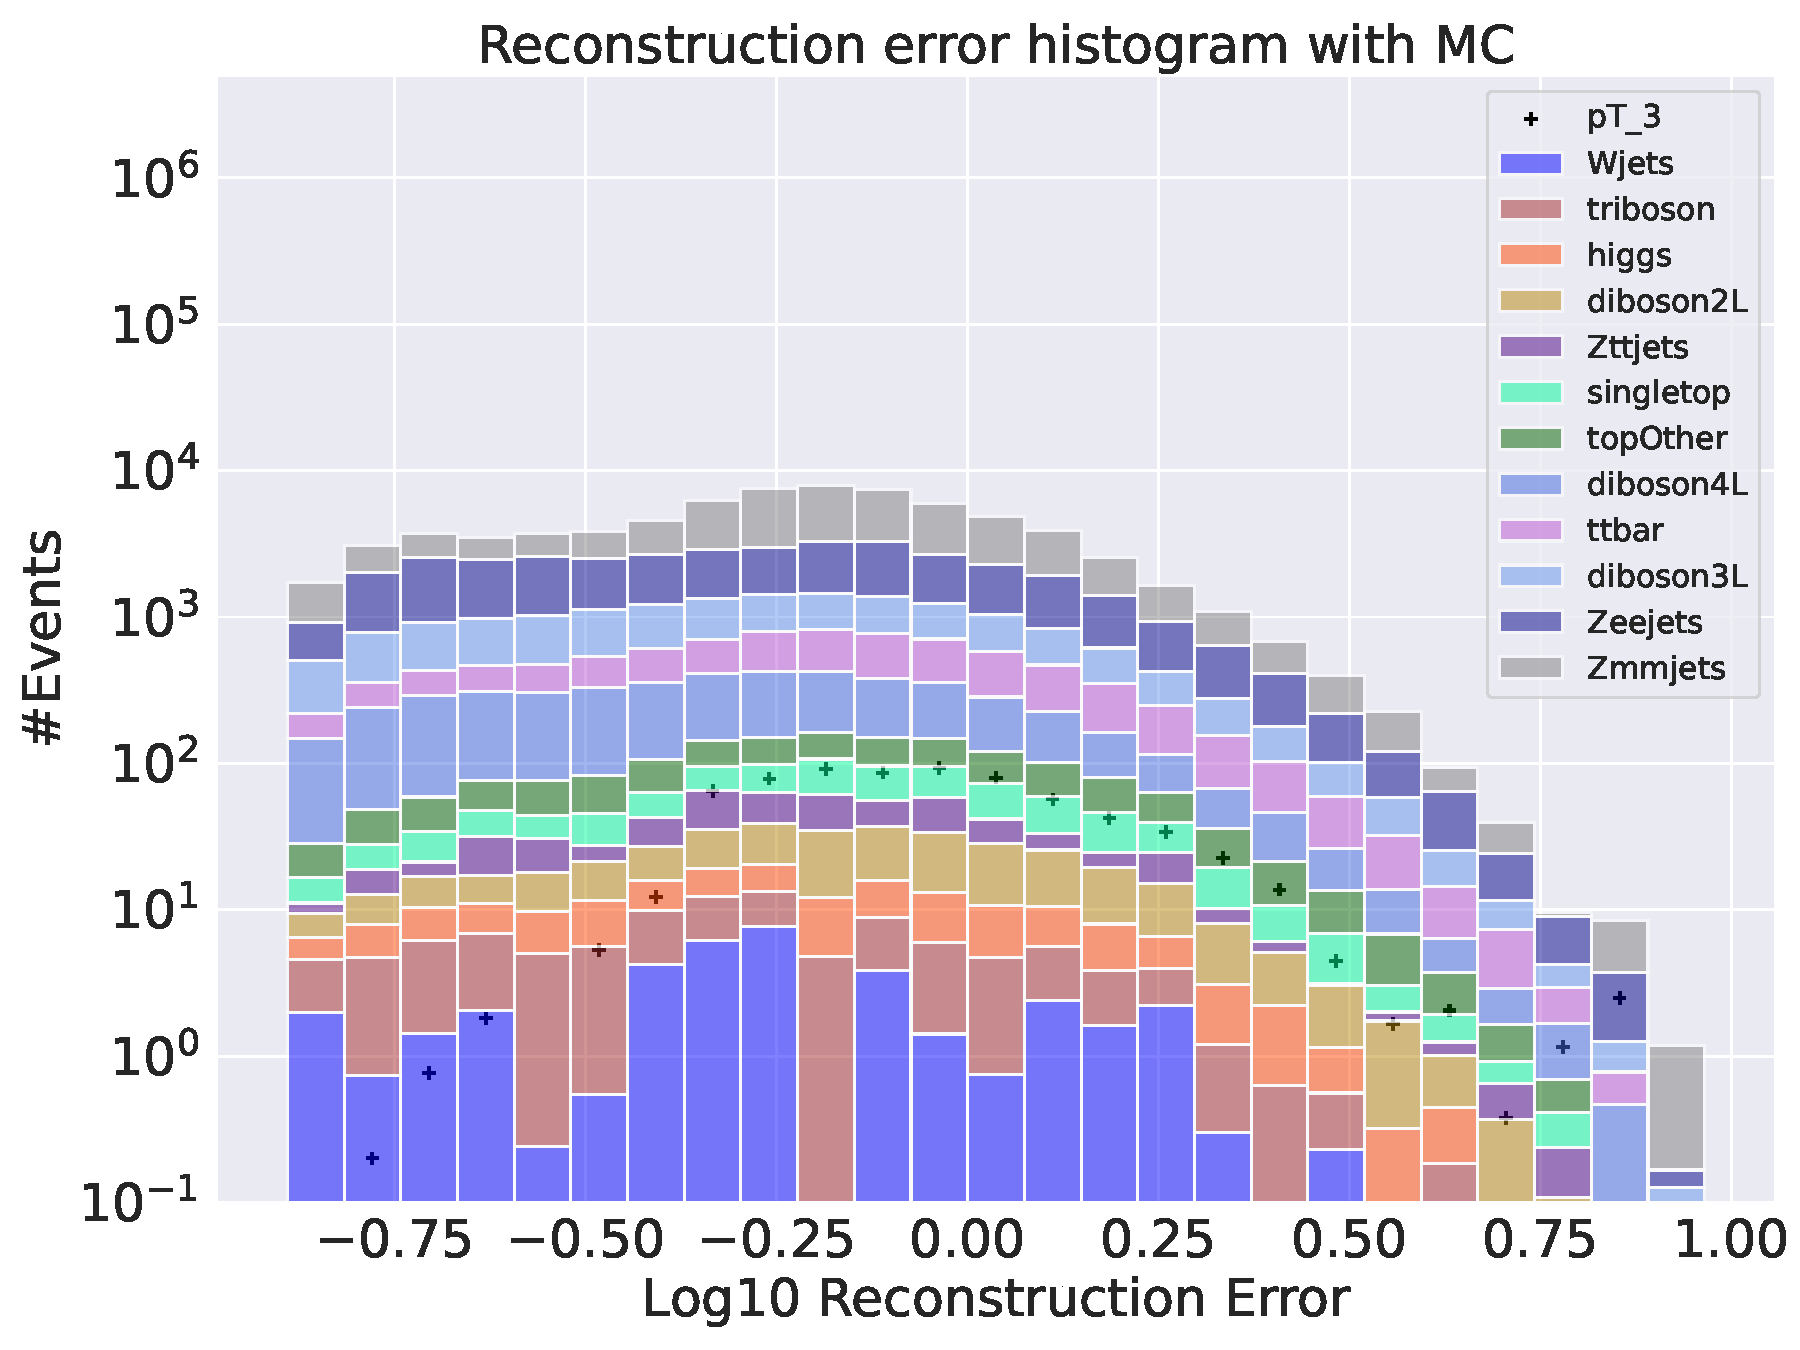
\includegraphics[width=\textwidth]{Figures/VAE_testing/small/b_data_recon_big_rm3_feats_sig_pT_3.pdf}
        \caption{Reconstruction error on validation SM MC from the small variational Autoencoder. Here the signal is a subsample of the validation 
        set where the transverse momentum of the first electron and the first muon has been increased with a scale of $3$. The change of transverse 
        energy has thusly also been changed according to the scaling of transverse momentum. No significant difference in distributions are found. }
        \label{fig:VAE_small_pt_3}
    \end{subfigure}
    \hfill 
    \begin{subfigure}{.45\textwidth}
        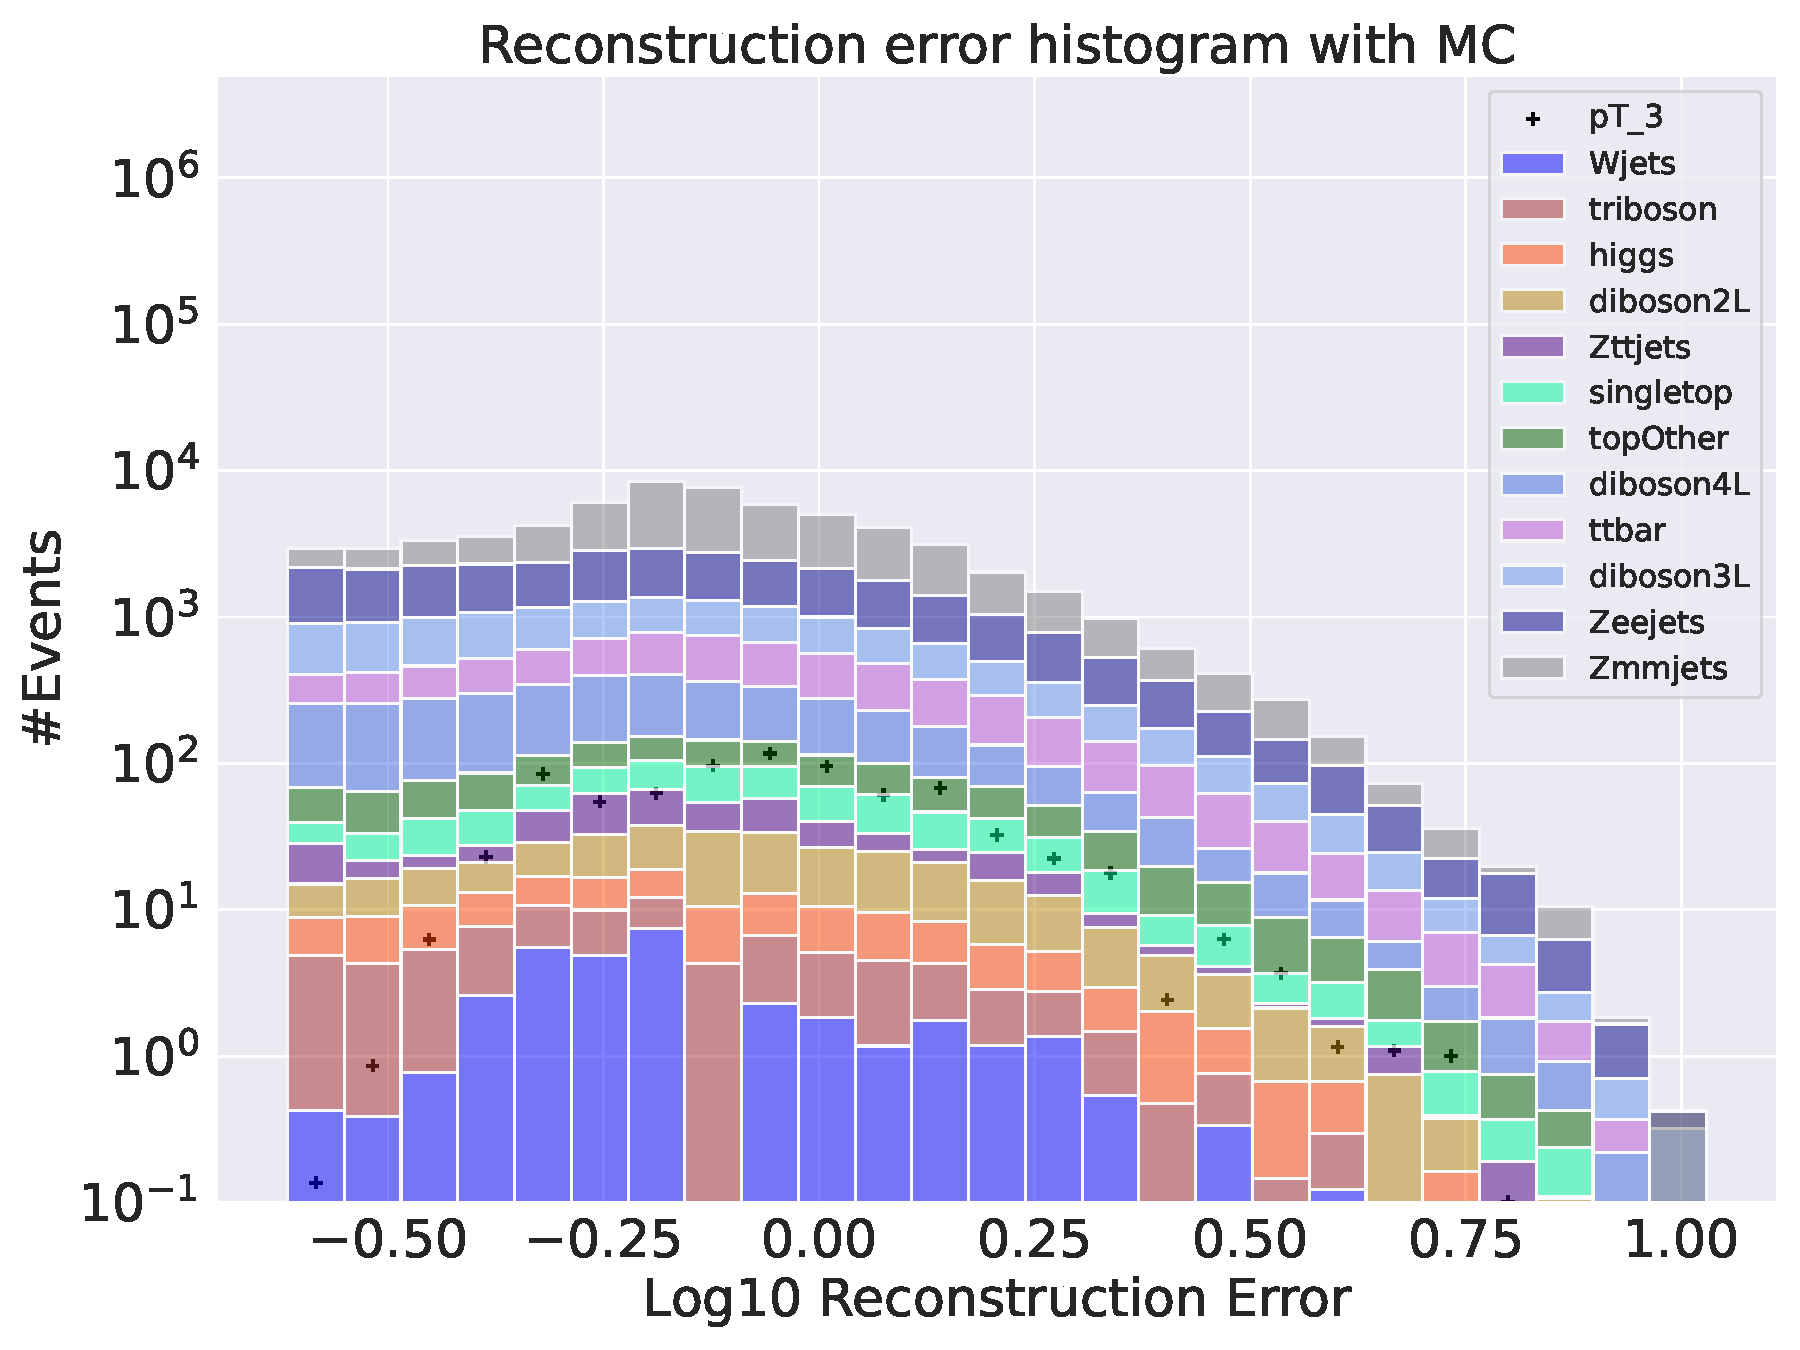
\includegraphics[width=\textwidth]{Figures/VAE_testing/big/b_data_recon_big_rm3_feats_sig_pT_3.pdf}
        \caption{Reconstruction error on validation SM MC from the big variational Autoencoder. Here the signal is a subsample of the validation 
        set where the transverse momentum of the first electron and the first muon has been increased with a scale of $3$. The change of transverse 
        energy has thusly also been changed according to the scaling of transverse momentum. No significant difference in distributions are found. }
        \label{fig:VAE_big_pt_3}
    \end{subfigure}
    \hfill 
    \caption{title}
    \label{fig:VAE_big_small_pt_3}
\end{figure}

\begin{figure}[h!]
    \centering
    \begin{subfigure}{.45\textwidth}
        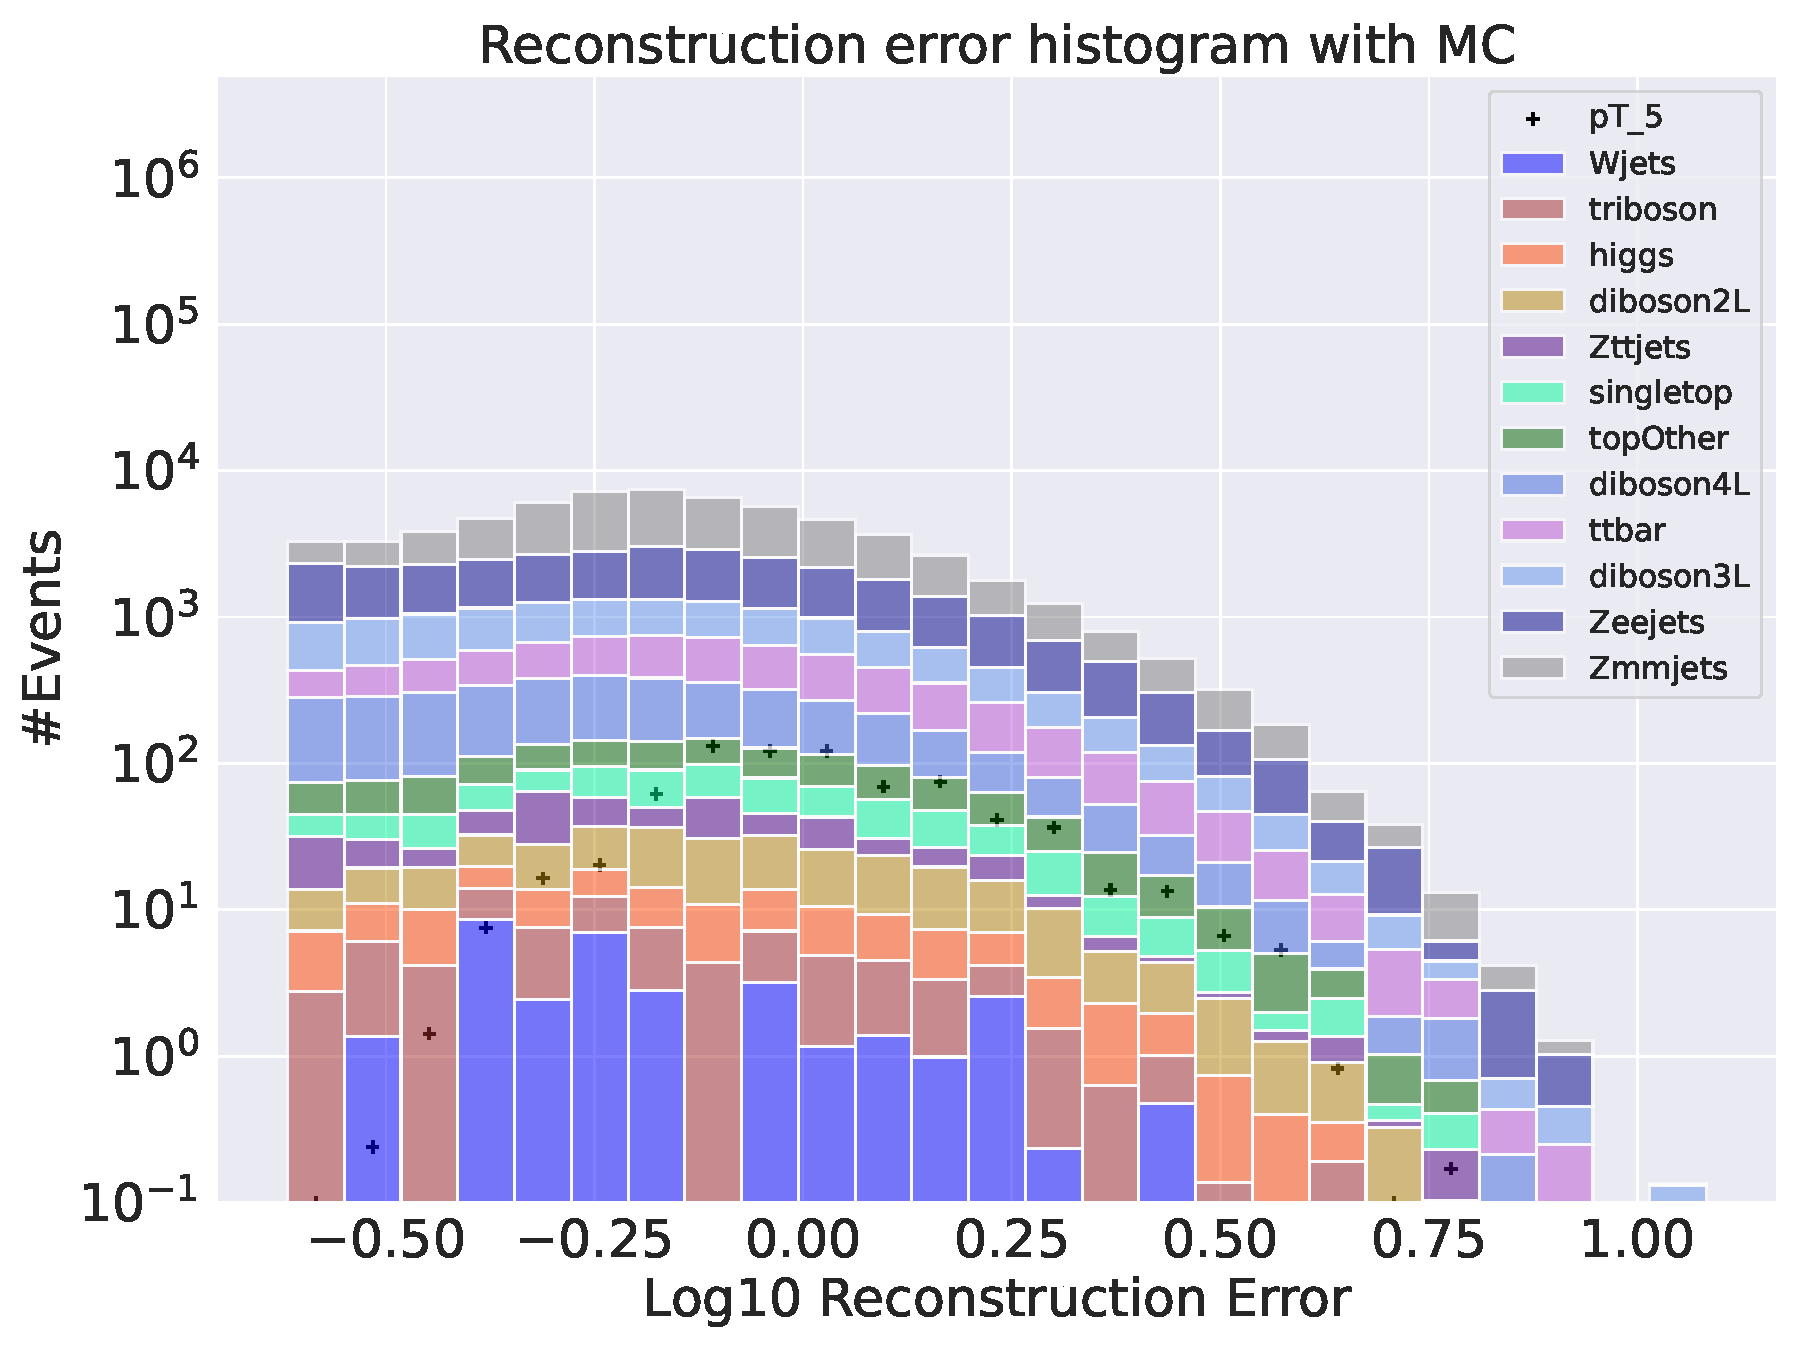
\includegraphics[width=\textwidth]{Figures/VAE_testing/small/b_data_recon_big_rm3_feats_sig_pT_5.pdf}
        \caption{Reconstruction error on validation SM MC from the small variational Autoencoder.Here the signal is a subsample of the validation 
        set where the transverse momentum of the first electron and the first muon has been increased with a scale of $5$. The change of transverse 
        energy has thusly also been changed according to the scaling of transverse momentum.  No significant difference in distributions are found. }
        \label{fig:VAE_small_pt_5}
    \end{subfigure}
    \hfill 
    \begin{subfigure}{.45\textwidth}
        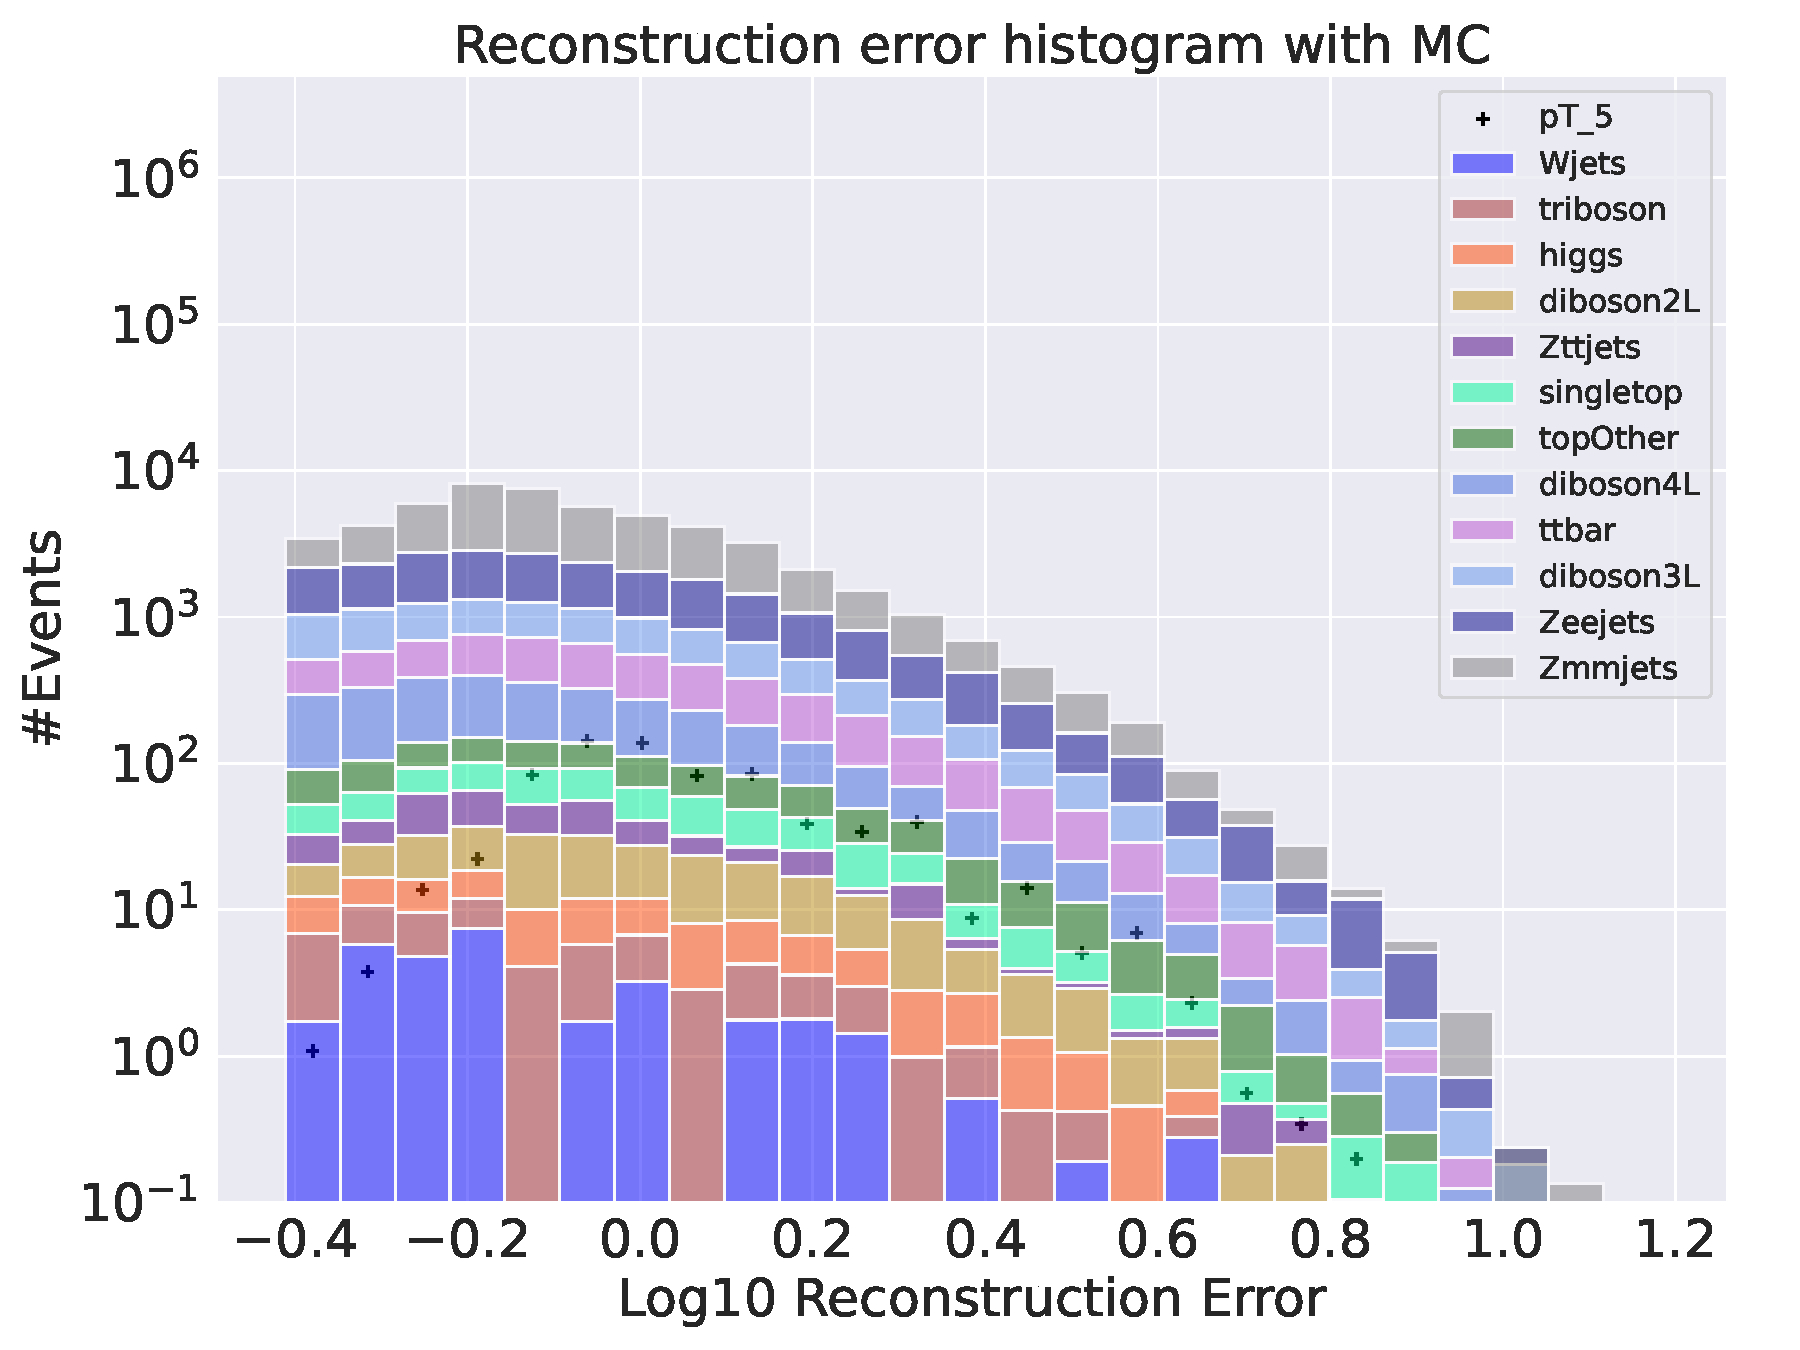
\includegraphics[width=\textwidth]{Figures/VAE_testing/big/b_data_recon_big_rm3_feats_sig_pT_5.pdf}
        \caption{Reconstruction error on validation SM MC from the big variational Autoencoder. Here the signal is a subsample of the validation 
        set where the transverse momentum of the first electron and the first muon has been increased with a scale of $5$. The change of transverse 
        energy has thusly also been changed according to the scaling of transverse momentum. No significant difference in distributions are found. }
        \label{fig:VAE_big_pt_5}
    \end{subfigure}
    \hfill 
    \caption{title}
    \label{fig:VAE_big_small_pt_5}
\end{figure}


\begin{figure}[h!]
    \centering
    \begin{subfigure}{.45\textwidth}
        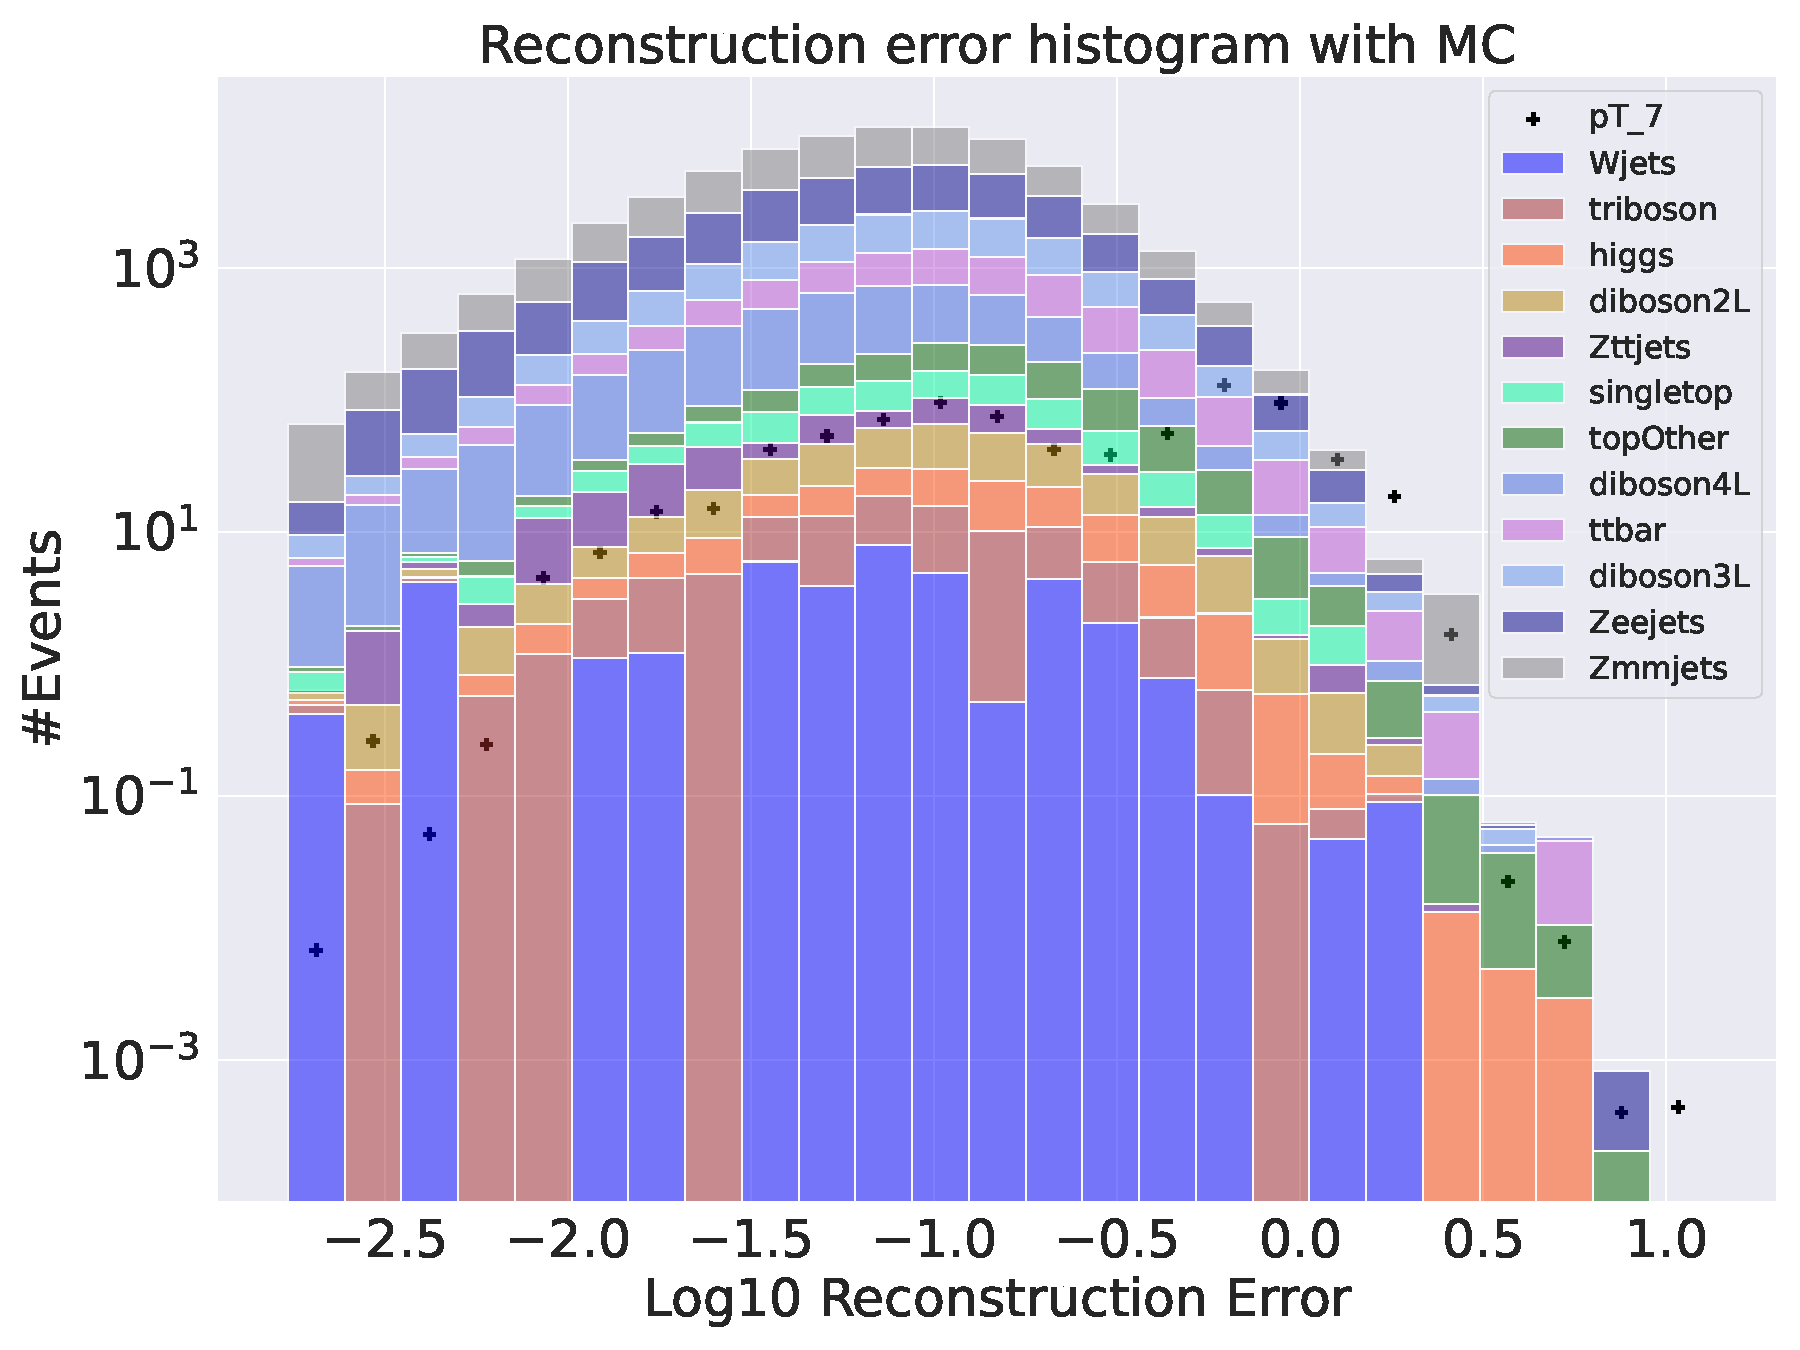
\includegraphics[width=\textwidth]{Figures/VAE_testing/small/b_data_recon_big_rm3_feats_sig_pT_7.pdf}
        \caption{Reconstruction error on validation SM MC from the small variational Autoencoder. Here the signal is a subsample of the validation 
        set where the transverse momentum of the first electron and the first muon has been increased with a scale of $7$. The change of transverse 
        energy has thusly also been changed according to the scaling of transverse momentum. No significant difference in distributions are found. }
        \label{fig:VAE_small_pt_7}
    \end{subfigure}
    \hfill 
    \begin{subfigure}{.45\textwidth}
        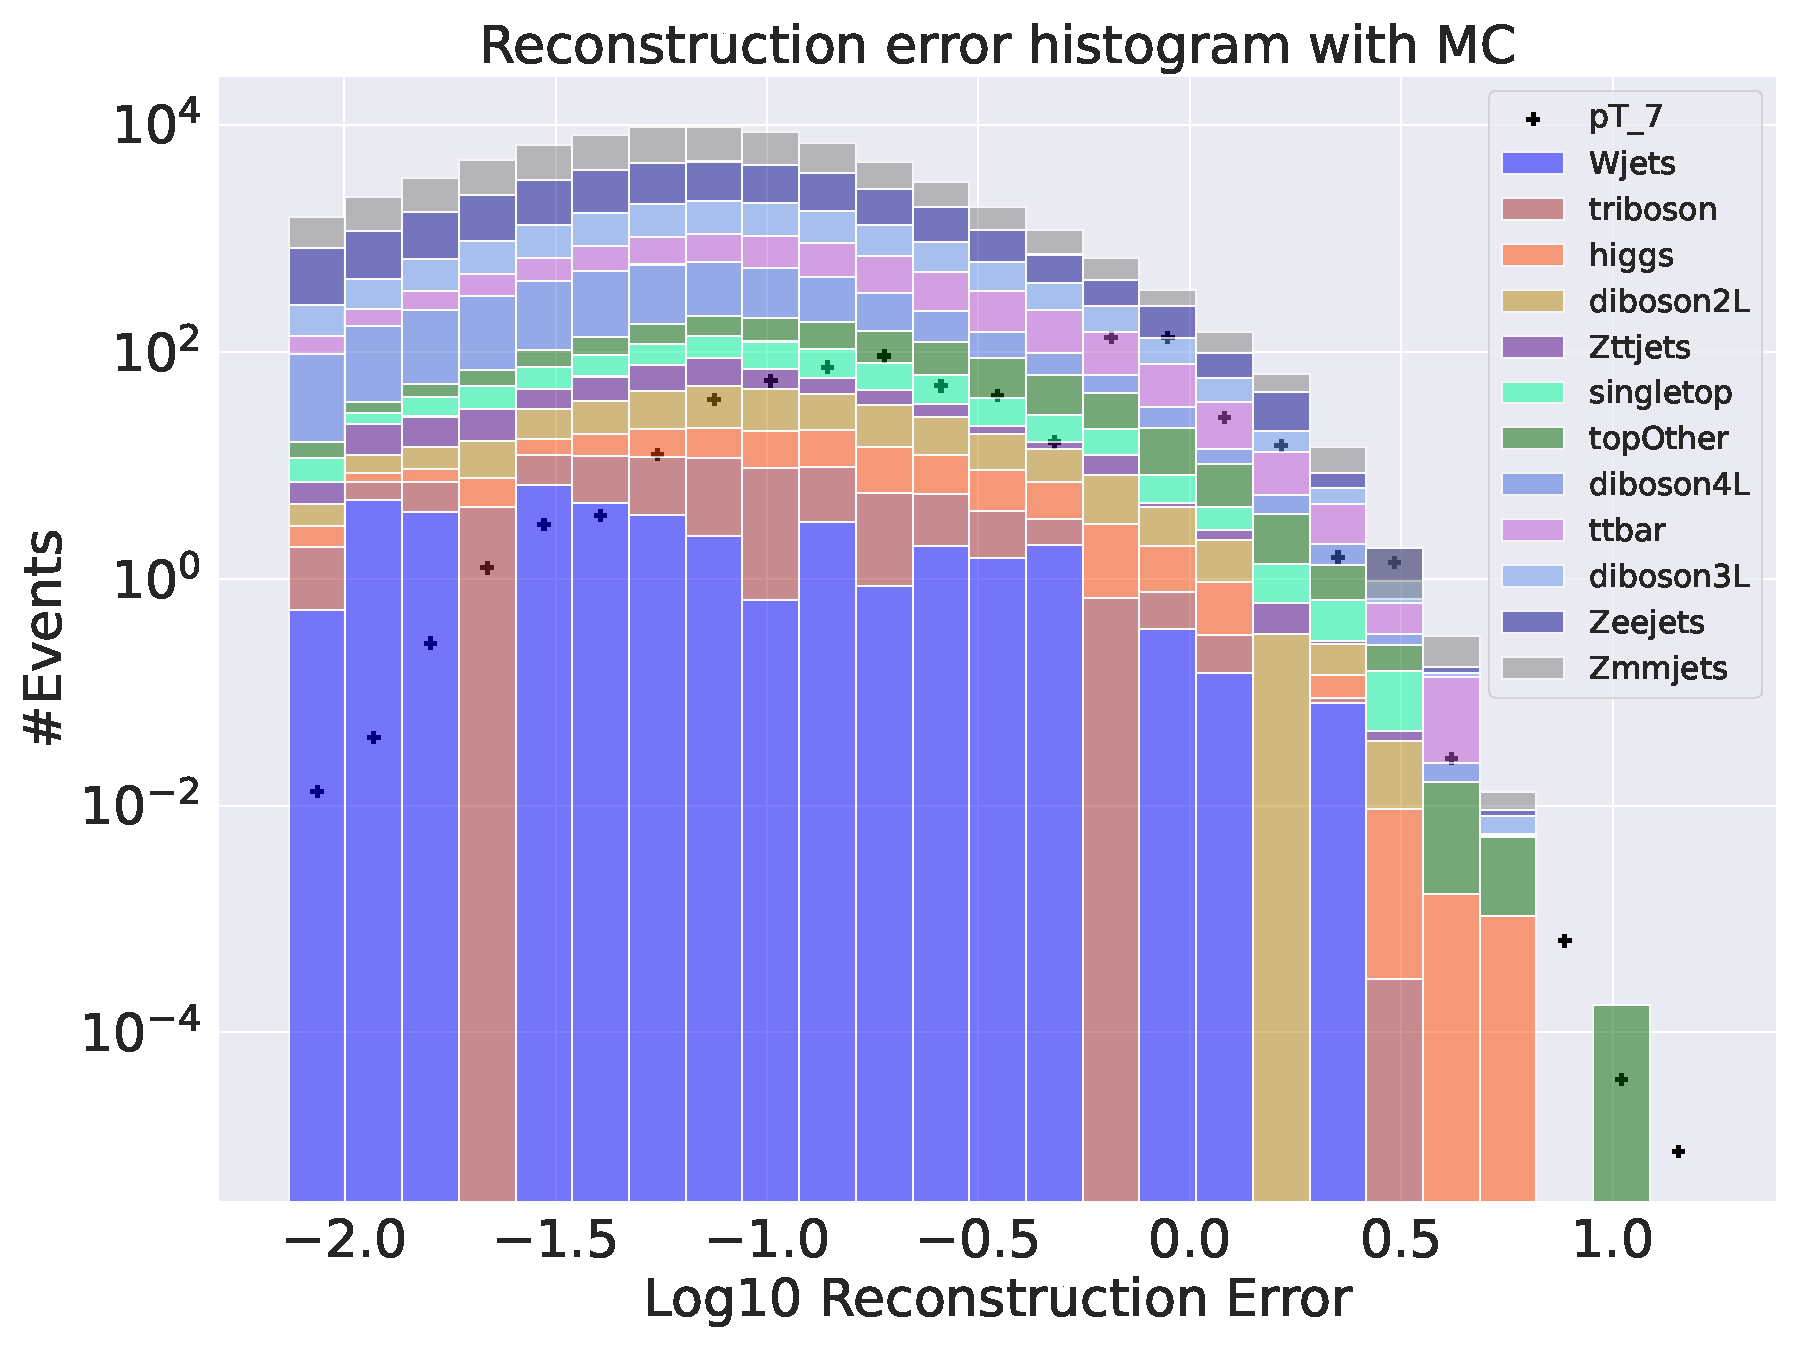
\includegraphics[width=\textwidth]{Figures/VAE_testing/big/b_data_recon_big_rm3_feats_sig_pT_7.pdf}
        \caption{Reconstruction error on validation SM MC from the big variational Autoencoder. Here the signal is a subsample of the validation 
        set where the transverse momentum of the first electron and the first muon has been increased with a scale of $7$. The change of transverse 
        energy has thusly also been changed according to the scaling of transverse momentum. No significant difference in distributions are found. }
        \label{fig:VAE_big_pt_7}
    \end{subfigure}
    \hfill 
    \caption{title}
    \label{fig:VAE_big_small_pt_7}
\end{figure}

\begin{figure}[h!]
    \centering
    \begin{subfigure}{.45\textwidth}
        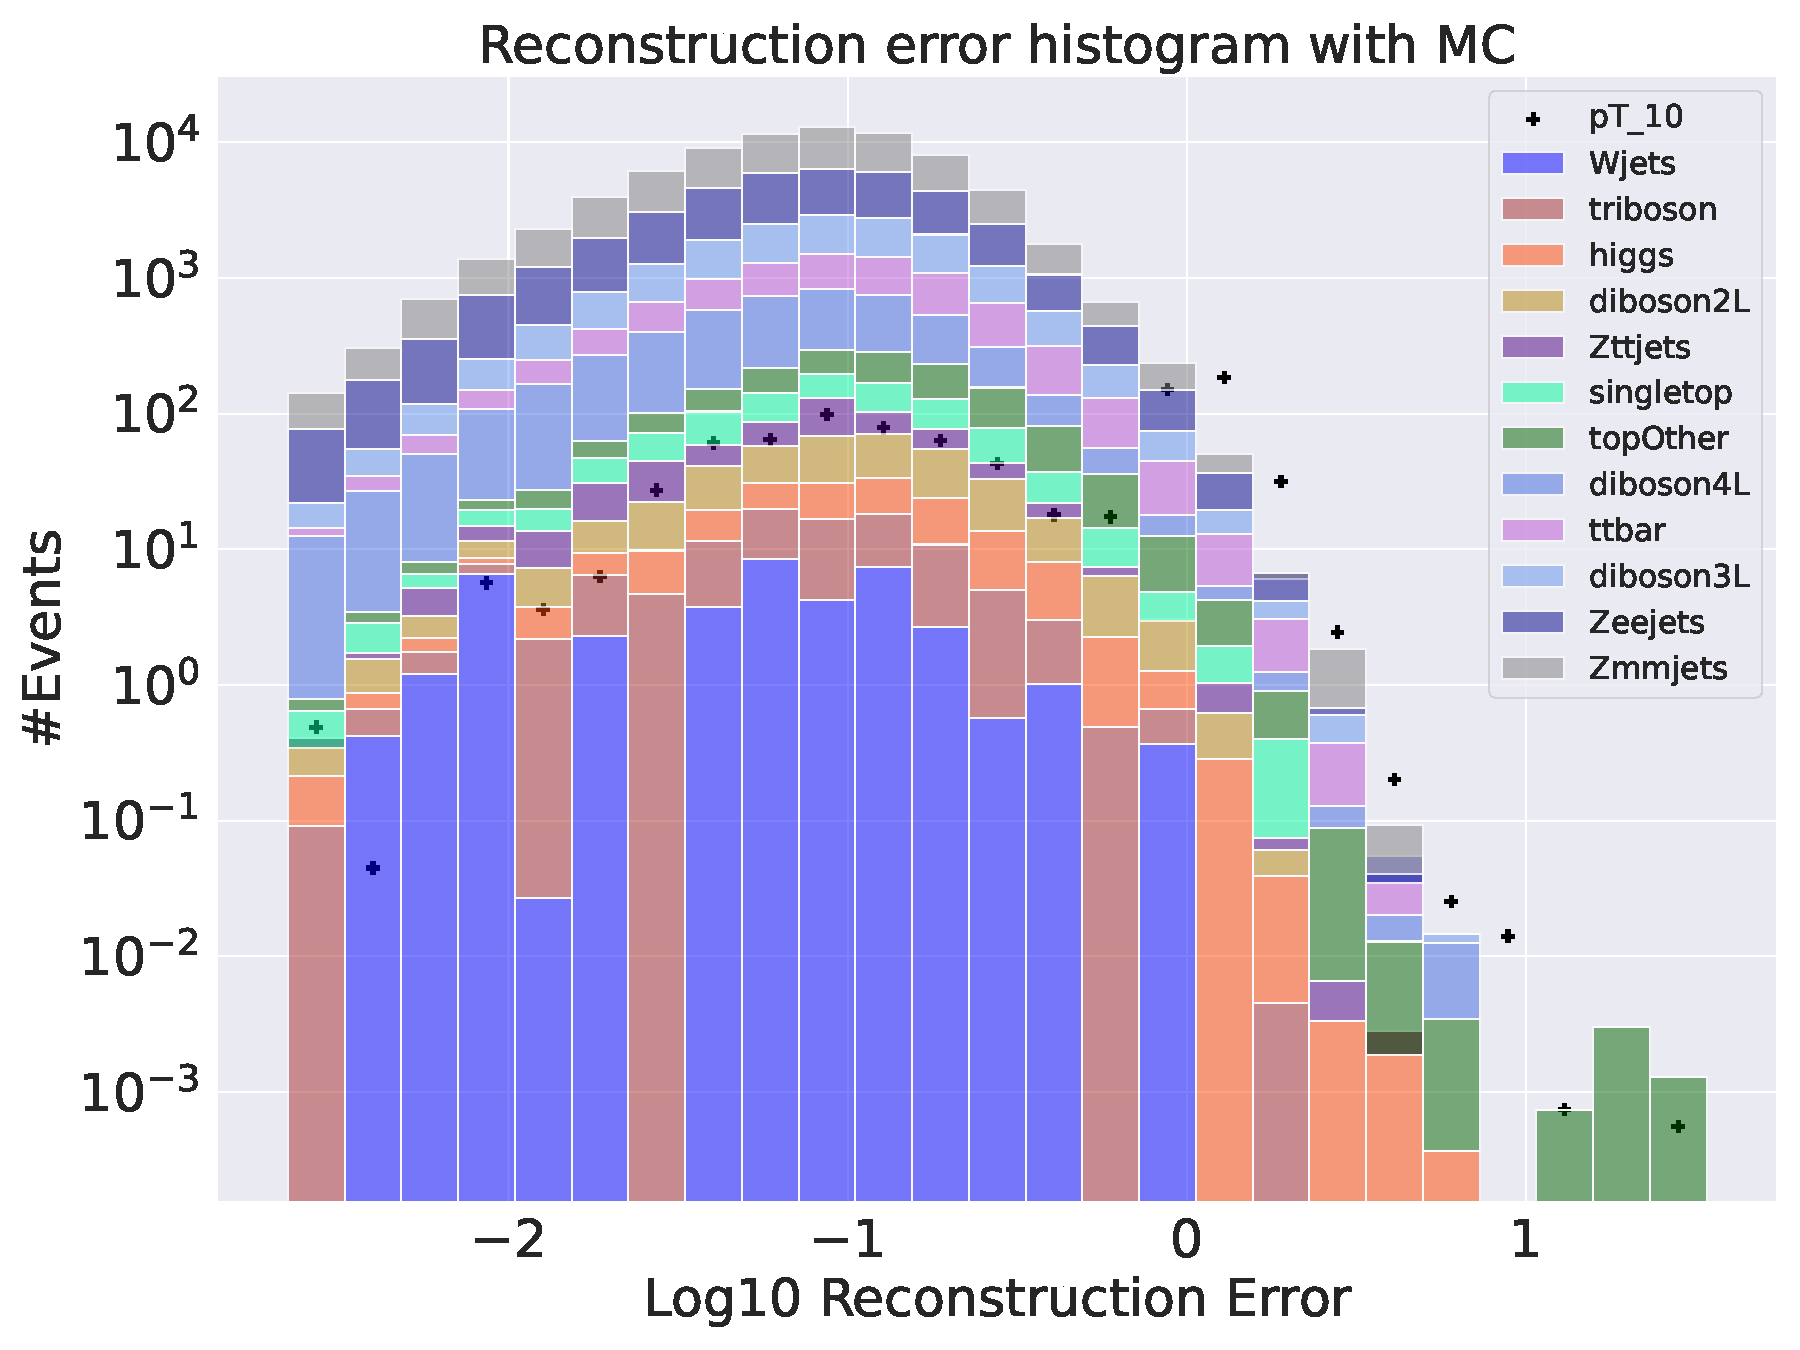
\includegraphics[width=\textwidth]{Figures/VAE_testing/small/b_data_recon_big_rm3_feats_sig_pT_10.pdf}
        \caption{Reconstruction error on validation SM MC from the small variational Autoencoder. Here the signal is a subsample of the validation 
        set where the transverse momentum of the first electron and the first muon has been increased with a scale of $10$. The change of transverse 
        energy has thusly also been changed according to the scaling of transverse momentum. No significant difference in distributions are found. }
        \label{fig:VAE_small_pt_10}
    \end{subfigure}
    \hfill 
    \begin{subfigure}{.45\textwidth}
        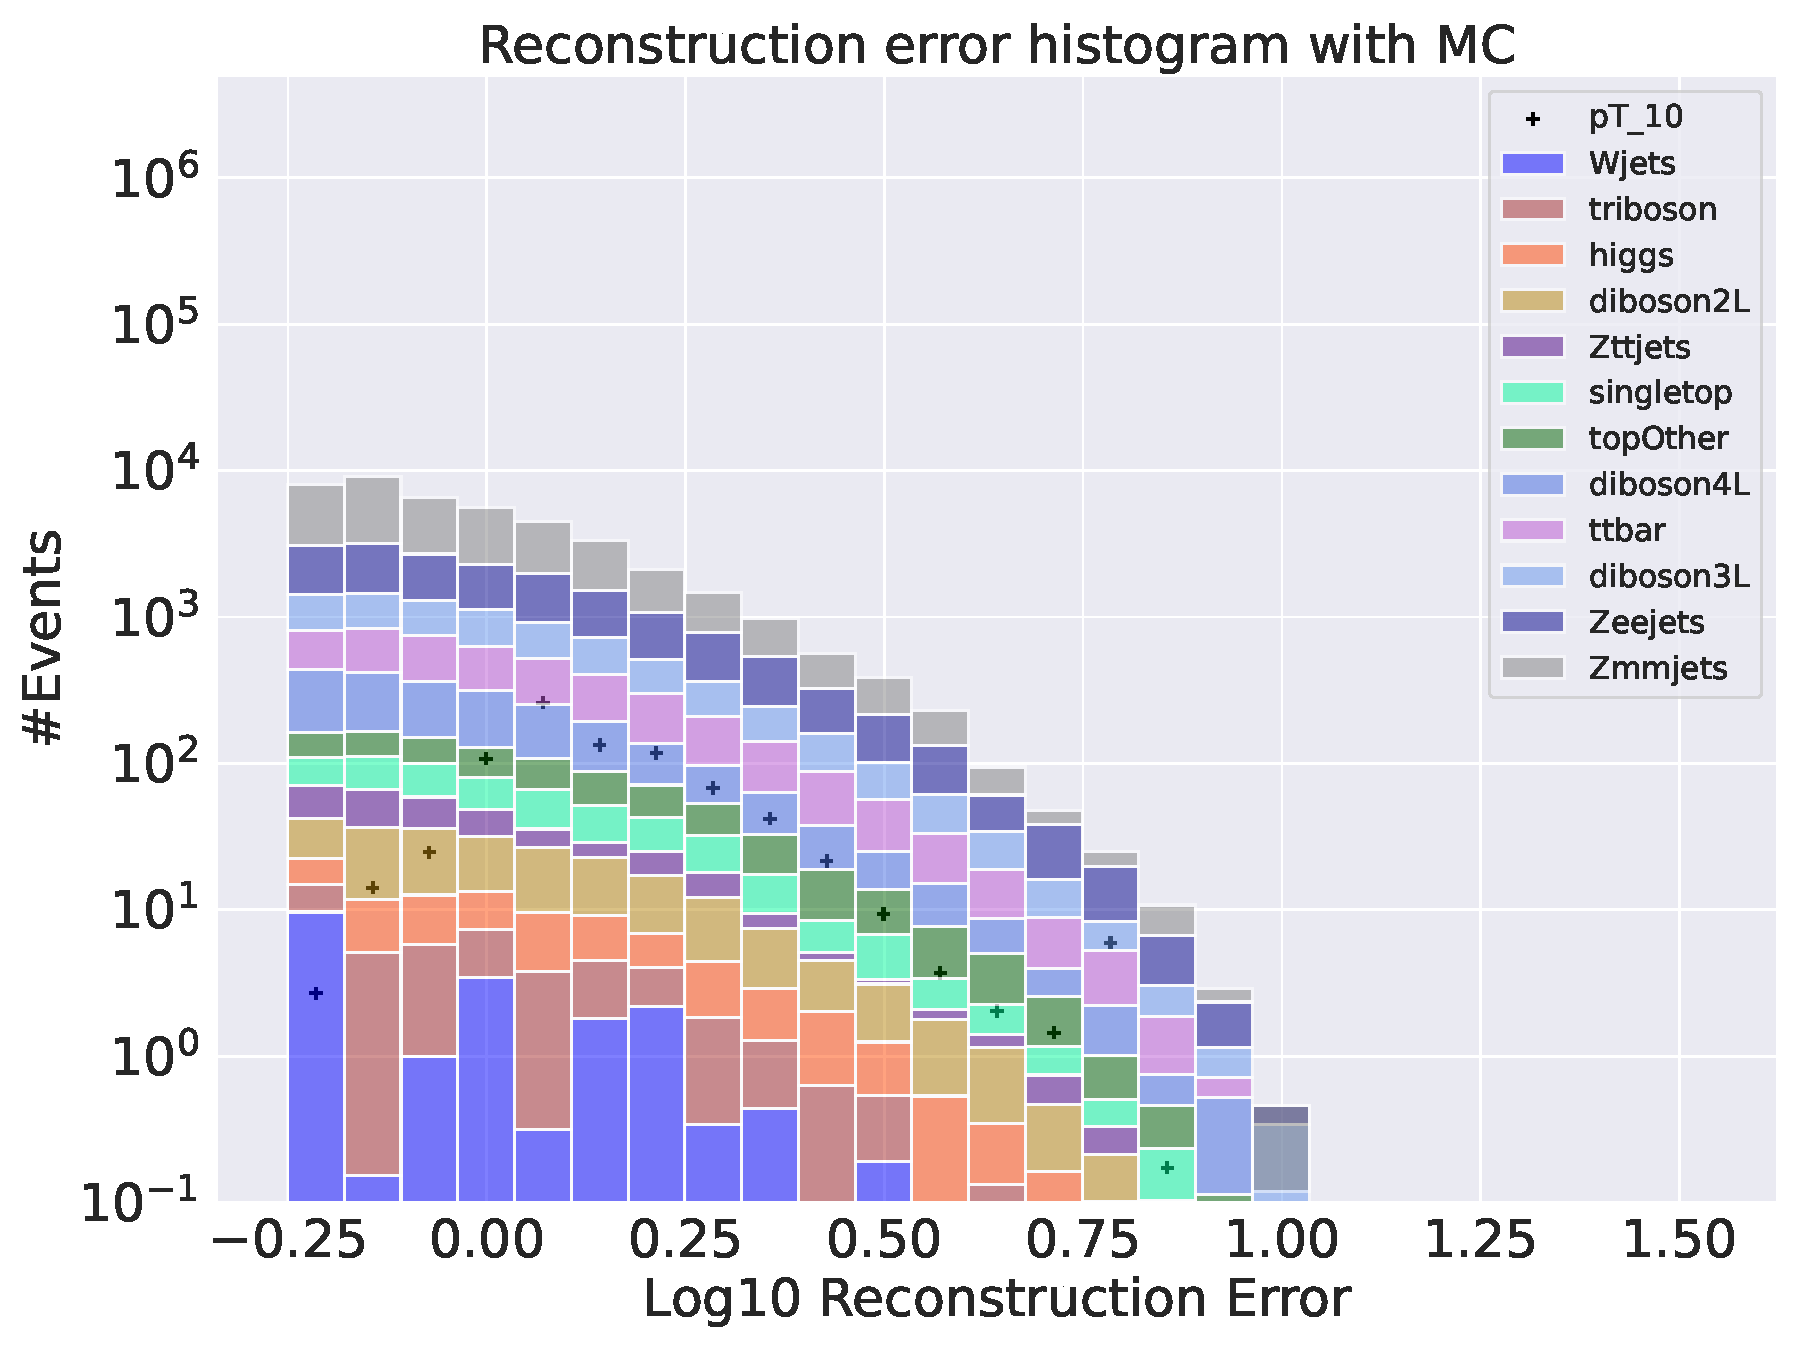
\includegraphics[width=\textwidth]{Figures/VAE_testing/big/b_data_recon_big_rm3_feats_sig_pT_10.pdf}
        \caption{Reconstruction error on validation SM MC from the big variational Autoencoder. Here the signal is a subsample of the validation 
        set where the transverse momentum of the first electron and the first muon has been increased with a scale of $10$. The change of transverse 
        energy has thusly also been changed according to the scaling of transverse momentum. No significant difference in distributions are found. }
        \label{fig:VAE_big_pt_10}
    \end{subfigure}
    \hfill 
    \caption{title}
    \label{fig:VAE_big_small_pt_10}
\end{figure}

\newpage